\documentclass[12pt, a4paper]{article}

\usepackage[a4paper,width=150mm,top=25mm,bottom=25mm,bindingoffset=6mm]{geometry}
\usepackage[T1]{fontenc} 	%Font 				
\usepackage[norsk]{babel}	 %Norske tegn
\usepackage[norsk]{datetime} %Dato på norsk
\usepackage[utf8]{inputenc}						
\usepackage{graphicx}       %Bilder	
\usepackage{siunitx}		%SI-enheter
\usepackage{pdfpages}		%Legge til PDF
\usepackage[title]{appendix}
\usepackage{hyperref}
%\usepackage{amsmath,amssymb}
%\usepackage{grffile}
%\usepackage{listings}
%\usepackage{caption}
%\usepackage[export]{adjustbox}
\usepackage{titling}		%Fancy - forside - opplegg


%\setcounter{secnumdepth}{0}


\setlength{\textheight}{240mm} 
\setlength{\textwidth}{180mm}  
\topmargin -5mm 
\oddsidemargin -5mm


%%%%%% Forside %%%%%%

\begin{document}

\begin{titlepage}

\newcommand{\HRule}{\rule{\linewidth}{0.5mm}} % Defines a new command for the horizontal lines, change thickness here

\center % Center everything on the page
 
%----------------------------------------------------------------------------------------
%	HEADING SECTIONS
%----------------------------------------------------------------------------------------

\vspace*{-3.5cm}\hspace*{-16cm}
\includegraphics{uitlogo.png}\\[3.0cm] % Include a department/university logo - this will require the graphicx package
\vspace*{-1.0cm}\textsc{\LARGE Universitetet i Tromsø}\\[2.5cm] % Name of your university/college
\textsc{\Large Praksis som valgemne}\\[0.5cm] % Major heading such as course name
\textsc{\large TEK-2000}\\[0.5cm] % Minor heading such as course title

%----------------------------------------------------------------------------------------
%	TITLE SECTION
%----------------------------------------------------------------------------------------

\HRule \\[0.4cm]
{ \huge \bfseries Rapport om praksis hos Norut}\\[0.4cm] % Title of your document
{\large \formatdate{14}{8}{2018} \hspace{1cm} - \hspace{1cm}\formatdate{10}{9}{2018}}\\[.55cm] % Date, change the \today to a set date if you want to be precise
\HRule \\[1.0 cm]

%----------------------------------------------------------------------------------------
%	AUTHOR SECTION
%----------------------------------------------------------------------------------------
\textbf{Institutt for ingeniørvitenskap og teknologi}\\
\hspace{-6.3cm} Fredrik Sandhei\\[.25cm] % Your name

%----------------------------------------------------------------------------------------
\begin{figure}[h!]
	\centering
	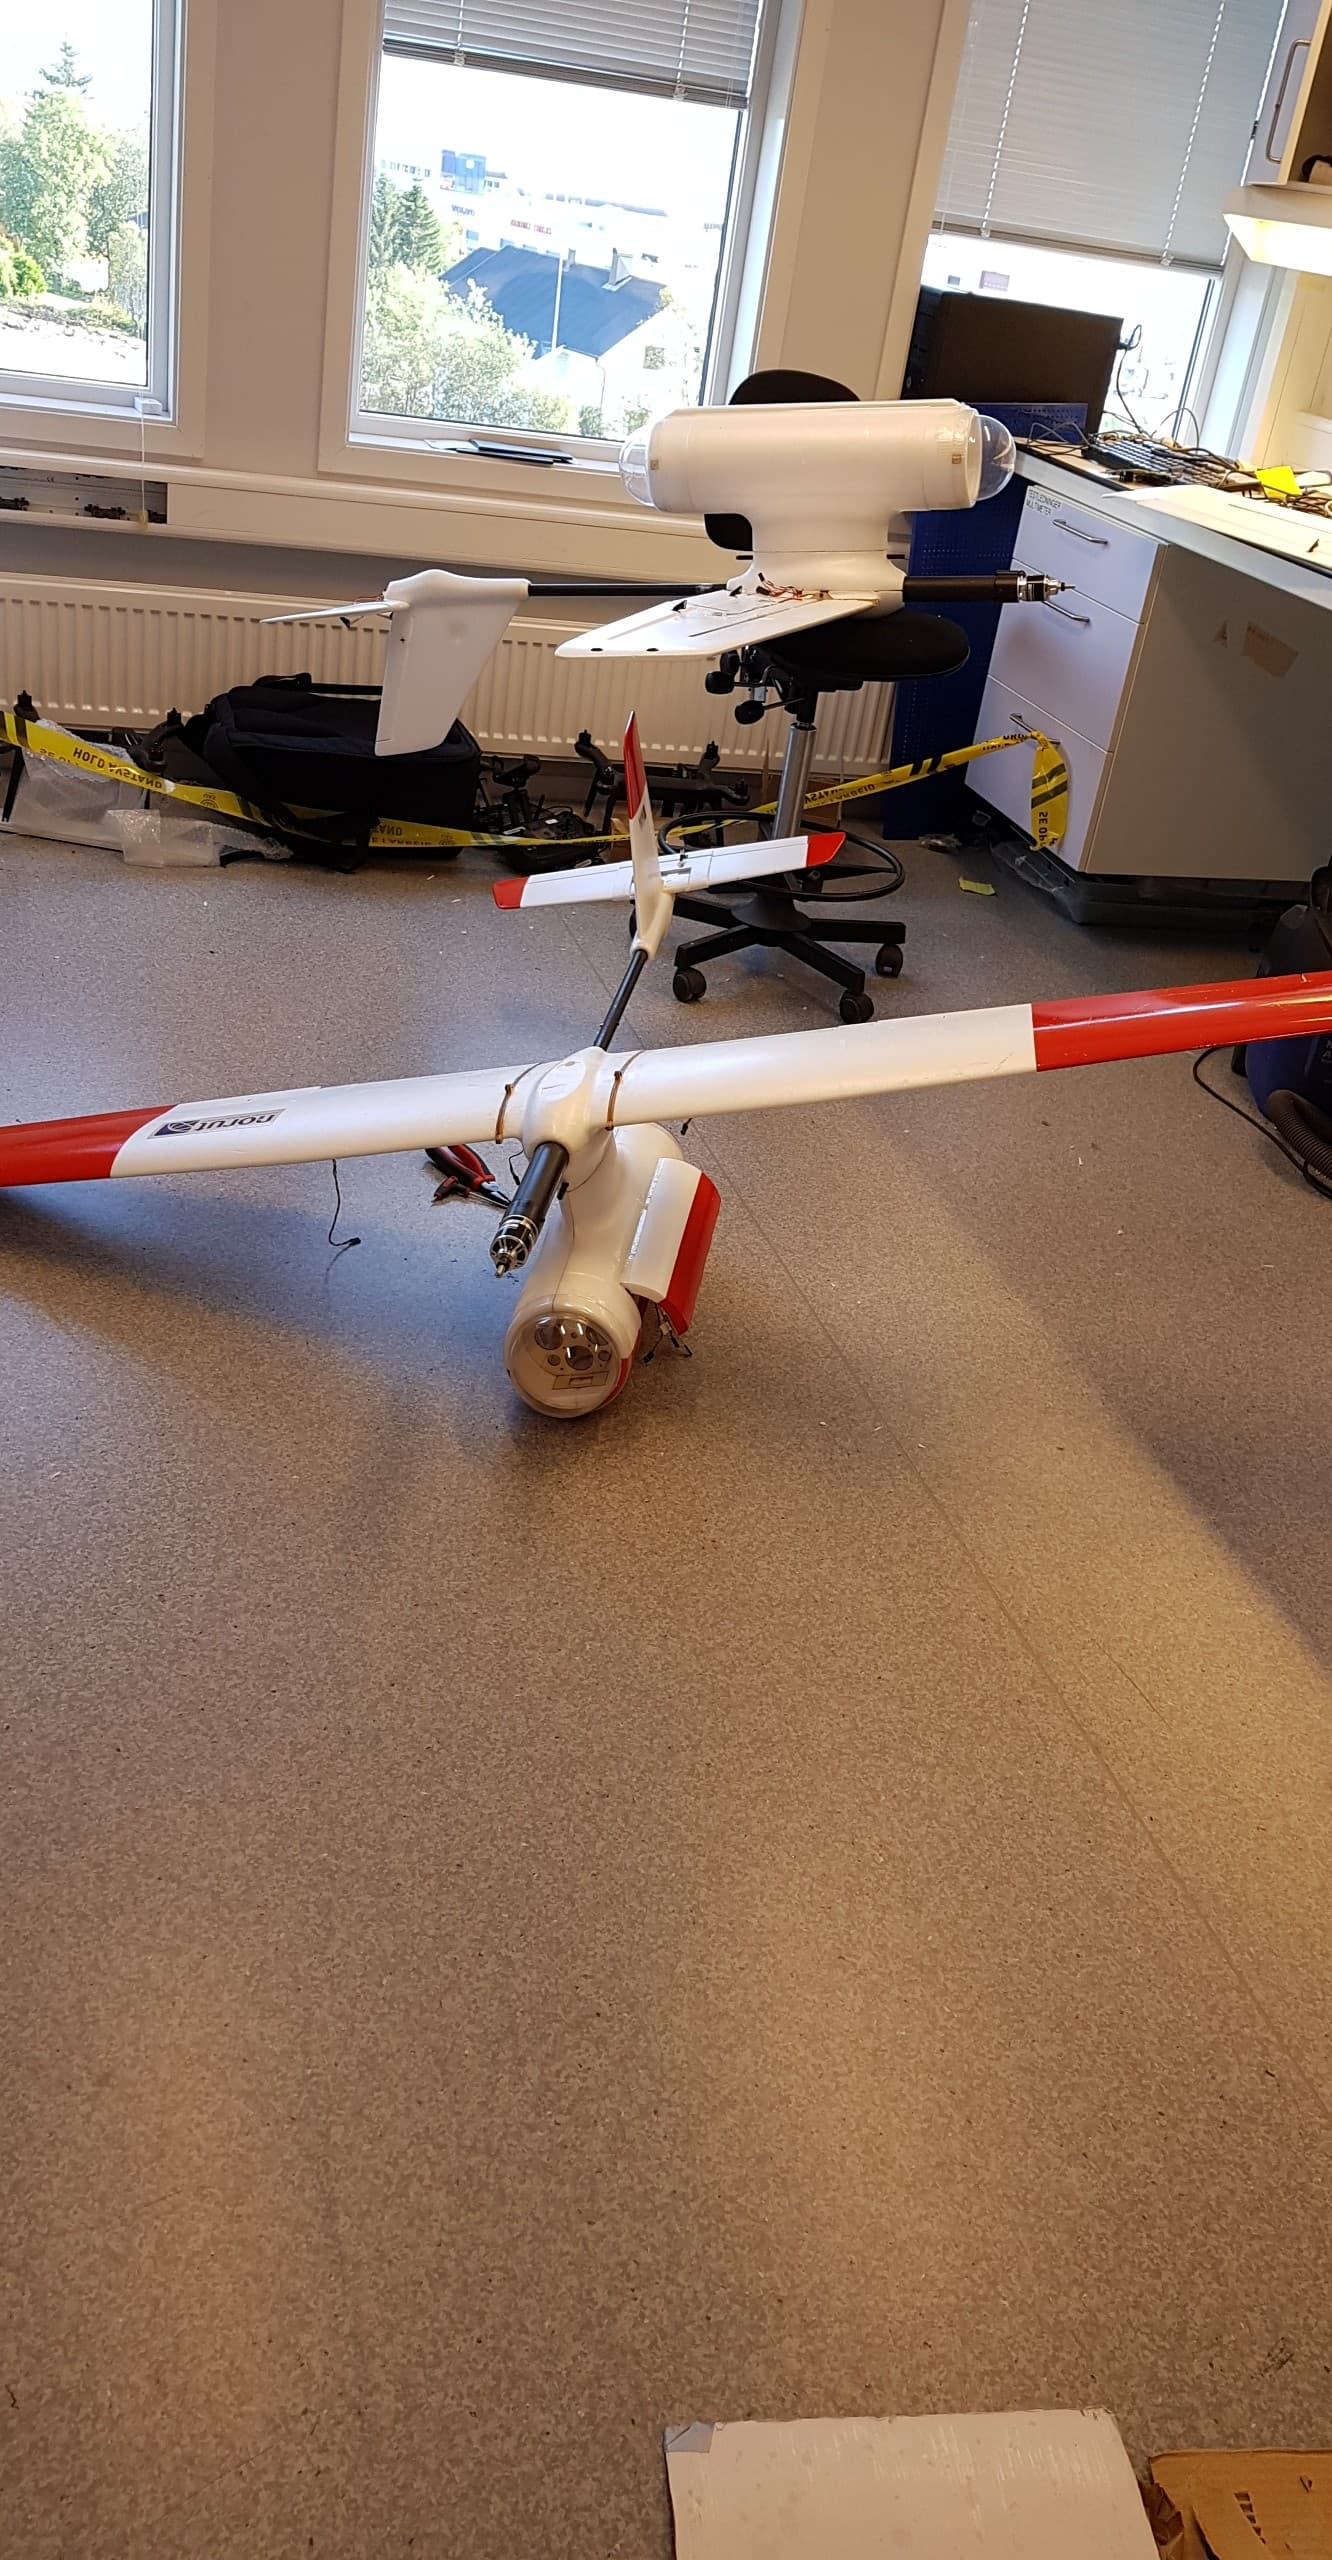
\includegraphics[width = 6cm, height = 9.3cm]{bilder/andre_fly_ferdigstilt.jpg}
\end{figure}
%----------------------------------------------------------------------------------------

\vfill % Fill the rest of the page with whitespace

\end{titlepage}
%%%%%% Slutt på forside %%%%%%

\date{\today}

%\maketitle
\clearpage

\section*{Prosjektrapport - Side 2}

\begin{tabular}{ | l | l | }
	\hline
	\textbf{Studieretning: Droneteknologi}\hspace{1.7cm} & \textbf{År: 2018} \hspace{2cm} \\
	\hline 
%	\vspace{1cm}
	\hline
	Tittel: \hspace{5cm} 			& Dato: \\
						 			& \\
	Rapport om praksis hos Norut	& Gradering: \\
    								& \\
						 			& Antall sider: \\
						 			& \\
						 			& Vedlegg: \\ \cline{1-1}
						 			& - Praksisplan \\
	Forfatter(e):		     			& - Logg av praksisperiode \\
	Fredrik Sandhei		 			& - CryoWing Observer Pilot Operating Handbook \\
									& - CryoWing Observer byggelogg \\	
						 			& - Strategi for å bestemme CryoWing\\ 
						 			& Observers egenskaper \\ 
						 			& - Attest fra Norut\\
						 			& \\						 
	\hline
	Fortrolighet: Fortrolig		 	& \\						 			
						 			& \\
						 			\hline
	Veileder:			 			& \\ 
	Arne Gjengedal 					& \\
									\hline 
	Oppdragsgiver: 		 			& Oppdragsgivers kontaktperson \\
	Norut					 		& Rune Storvold \\
						 			& \\
						 			& \\
	\hline
\end{tabular}
\vspace{.25cm}

\begin{flushleft}
	\begin{tabular}{ | l | }
		\hline
		Sammendrag: \hspace{14.7cm}
		\\
		Rapporten omhandler min praksisperiode hos Norut. Hovedoppgaven min var \\ å bygge og dokumentere tre fly av typen CryoWing Observer. \\
		Ting gikk ikke helt som planlagt. Dermed ble bare to fly bygd og jeg fikk ikke\\
		muligheten til å gjennomføre testflygning og dermed dokumentere\\ flyene.
		Jeg har likevel lært mye praktisk som 
		jeg kan ta videre i \\utdannelsen og arbeidslivet.
		\\
		\hline
		Stikkord: \\ Praksis, Norut, CryoWing Observer, droneteknologi\\ \\ \\ \\
		\hline
	\end{tabular}
\end{flushleft}

\clearpage


\section*{Sammendrag}
Denne rapporten omhandler min praksisperiode hos UAV-avdelingen til Norut i Tromsø. Jeg gjennomførte praksisperioden min i begynnelsen av høstsemesteret 2018, hvor jeg var 4 uker i strekk hos Norut. \\

Hovedoppgaven jeg fikk var å produsere tre CryoWing Observer fixed-wings, der én av disse skulle være en RC-trainer, mens de to andre skulle utstyres med autopilotsystem inkludert andre periferier. I tillegg til dette skulle jeg dokumentere flyenes luftdyktighet ved å testfly dem og fylle ut flyets egenskaper.\\

Flyene ble bygd ved å følge en bruksanvisning. Da jeg hadde svært lite erfaring med bygging fra før, var det å følge bruksanvisningen slavisk. \\

Mangel på opplæring og uregelmessig oppfølging samt lite tilgjengelighet på utstyr og personell gjorde at arbeidet tok lengre tid enn forventet. Dagene ble dermed stressende i og med at tre fly skulle bygges. Det ble besluttet at det var nok å få bygget to og i hvert fall få testflydd det ene flyet. \\

To fly ble ferdigbygd og det ene ble testflydd. Dessverre havarerte flyet i testflygning. Det var ikke mulighet å gjøre mer, da jeg ble ferdig med praksisen den samme dagen. \\

Til tross for det jeg oppfattet som stressende dager, har jeg lært mye, men på den ``harde måten''. Jeg har fått lært mye innenfor teknisk med tanke på struktur, komposittmaterialer i form av epoxy-lim og anvendelse av teori fra studiet. Hovedoppgaven har vært svært relevant med utdannelsen, og har gitt meg en god smak på hva som kan være i vente når jeg kommer ut i arbeidslivet som droneingeniør. \\

\clearpage
\section*{Forord}
TEK-2000 `Praksis som valgemne' er et av de tre emnene jeg har valgt for 5.semesteret mitt på 3.året i droneteknologi. Emnet går ut på at studenten skal ha en praksis hos en bedrift som er passende til utdannelsen. Praksisplassen må fylle kriterier fra emneansvarlig på bedriftens relevans til utdannelsen. \\

Jeg søkte praksis hos to plasser, Luftfartstilsynet og Norut. Begge er relevante på hver sin måte. Jeg fikk innpass hos begge, men på grunn av lokalitet valgte jeg Norut.\\

Denne rapporten beskriver min praksisperiode i UAV-avdelingen til Norut i Tromsø, hovedoppgaven min, og hvordan jeg har løst denne, inkludert mine refleksjoner av perioden. Da rapporten inneholder vedlegg som er stemplet fortrolig av Norut, er rapporten fortrolig, og skal leses av sensor og emneansvarlig. \\ 

Takk til Norut i Forskningsparken i Tromsø for at jeg fikk muligheten til å kunne gjennomføre praksisen min hos dem. Takk til forskningssjef Rune Storvold og resten av UAV-avdelingen for min tid der. Takk til UiT for å gi muligheten til studentene å ta dette emnet, og spesielt takk til emneansvarlig, Arne Gjengedal, som godkjente praksisen min hos Norut og har gitt veiledning til utarbeidingen av denne rapporten. \\[7cm]
%\vspace{7cm}
Tromsø, \today \\[.5cm]

Fredrik Sandhei\\

\begin{flushleft}
	\begin{tabular}{@{}p{.5in}p{4in}@{}}
	Signatur: & \hspace{.5cm}\textbf{Fredrik Sandhei} \\
			  & \hrulefill \\
	\end{tabular}

\end{flushleft}

%%%%%%%%%%%%%%%%%%%%%%%%%%%%%%%%%%%%%%%%%%%%%%%%%%%%%%%%%%%%%%%%%%%%%%%
							%Innholdsfortegnelse
%%%%%%%%%%%%%%%%%%%%%%%%%%%%%%%%%%%%%%%%%%%%%%%%%%%%%%%%%%%%%%%%%%%%%%%
\clearpage

\tableofcontents
% IKKE BRUK CLEARPAGE HER.. DET FUCKER OPP HELE FILAS LOOP...
\newpage
\listoffigures

\clearpage


\section{Innledning}
I begynnelsen av høstsemesteret 2018 begynte jeg en praksisperiode hos Norut i samsvar med emnet TEK-2000, hvor jeg var i fire uker. Min oppgave for denne perioden har vært å bygge tre fly på bestilling av Norut. I tillegg til dette har jeg vært litt i flere områder på avdelingen for ubemannede luftfartøy (UAV-avdelingen) og hjulpet litt rundt med reparasjonsarbeid og papirarbeid. Formålet med denne praksisperioden var å få et innblikk i hvordan et typisk arbeidsliv til en droneingeniør kan være. \\

I løpet av vårsemesteret 2018 var jeg innom Norut og snakket med avdelingssjefen på UAV - Rune Storvold - om muligheten for praksis. Han fortalte at det var arbeid som de hadde ønsket å få gjort, men som de selv ikke hadde kapasitet til for øyeblikket. Jeg har hatt interesse for modellflyging helt siden barndommen, men har aldri bygget et før, bortsett fra et par multirotorer.\\

Jeg var samtidig spent og gledet meg til å få gjøre dette. Tanken å få bruke det man har lært opp til nå gjennom studiet syntes jeg virke svært spennende. Erfaringene mine hos Norut kommer jeg til å ta med meg videre i utdannelsen min og det kommende arbeidslivet. 


\newpage
\section{Om arbeidsplassen}
\subsection{Norut}

Norut Northern Research Institute AS, eller Norut, er et nasjonalt forsknings- og innovasjonsselskap som produserer anvendbar, nordområderelevant kunnskap innen teknologi og samfunnsvitenskap. Selskapet ble dannet i 1992 og er majoritetseid av Universitetet i Tromsø. Norut har kontor i Alta, Bodø, Harstad og Bardu, med hovedkontor i Tromsø. \\

Som en forskningsvirksomhet er Norut delt inn i ulike forskningsområder. Disse områdene strekker fra arktisk teknologi, mineral-og prosessteknologi, fornybar energi til mye mer. De ulike forskningsområdene kommer av de muligheter og utfordringer som kommer av å være så langt nord. Det harde klimaet og landskapet gir Norut flere områder å forske på for å kunne produsere kunnskap og teknologi som er til nytte for samfunnet [1]. \\ 

Norut er kjent for å bruke ubemannet luftfartøy (UAV) til deres vitenskapelige formål, spesielt innenfor satellitt- og fjernmålingsteknologi. De har brukt UAV lenge før det ble mer eller mindre nasjonalt anerkjent av Luftfartstilsynet.\\

Bruk av UAV er en forholdsvis ny plattform for datainnhenting. Å bruke UAV er betydeligere billigere med tanke på materialer og ressurser enn ved bruk av bemannet luftfartøy. Ved at ingen personer er om bord i luftfartøyet ved flyging, reduseres risikoen for personskade, og oppdrag som kan være utfordrende å gjøre blir forenklet med bruk av UAV. \\

UAV-avdelingen som jeg tilbringte min tid hos Norud på, bruker UAV til for eksempel landmåling, sensordatainnhenting eller telling av dyr. Dataen som avdelingen samles kan sendes videre til en annen avdeling hos Norut eller videre til en annen bedrift som har bestilt tjenester fra UAV-avdelingen. \\

Da det foreløpig ikke er satt ordentlige standarder til drift av ubemannet luftfart, har Norut egne rutiner på drift og vedlikehold som de selv har satt. På grunn av Noruts erfaring med UAV, bidrar Norut med ressurser og opplæring av studentene på droneteknologi-utdanningen hos UiT. \\


Norut har en flåte av luftfartøy med kombinasjon av multirotorer og fixed-wing fly. Flyene er døpt til CryoWing, der noen av skrogene er importert fra Slovakia, og avionikken, motorsystem og annet er montert av Norut. Enkelte fly og multirotorer er byggesett som Norut selv har satt sammen eller er hyllevarer. De ulike fartøyene brukes til ulike formål der det er passende, deriblant landmåling og fjernmåling.\\
\newpage

\subsection{Noe av flåten}
Alle bildene her er med tillatelse av Rune Storvold fra Norut. \\ 
De ulike luftfartøyene som Norut innehar brukes til formål som landmåling, innhenting av sensordata fra luft, telling av eksempelvis isbjørner, og mer. Valget av luftfartøy avhenger av omfanget av oppdraget. Dersom det er store områder som skal dekkes, er det behov for et luftfartøy som kan dekke store avstander på relativt kort tid og kan kunne være i luft over lengre tid. For slike oppdrag er det gunstig å bruke fixed-wings, altså fly. Slike type oppdrag kan være kartlegging av oljesøl[6] \\
Visse oppdrag kan være over mindre områder, men det kreves helst finere presisjon på sluttproduktet, for eksempel ved linjeinspeksjoner. Da er det gunstig å benytte multirotorer for å kunne komme nærmere inn på hver stolpe for grundigere inspeksjon. 

\begin{figure}[hpbt]
	\centering
	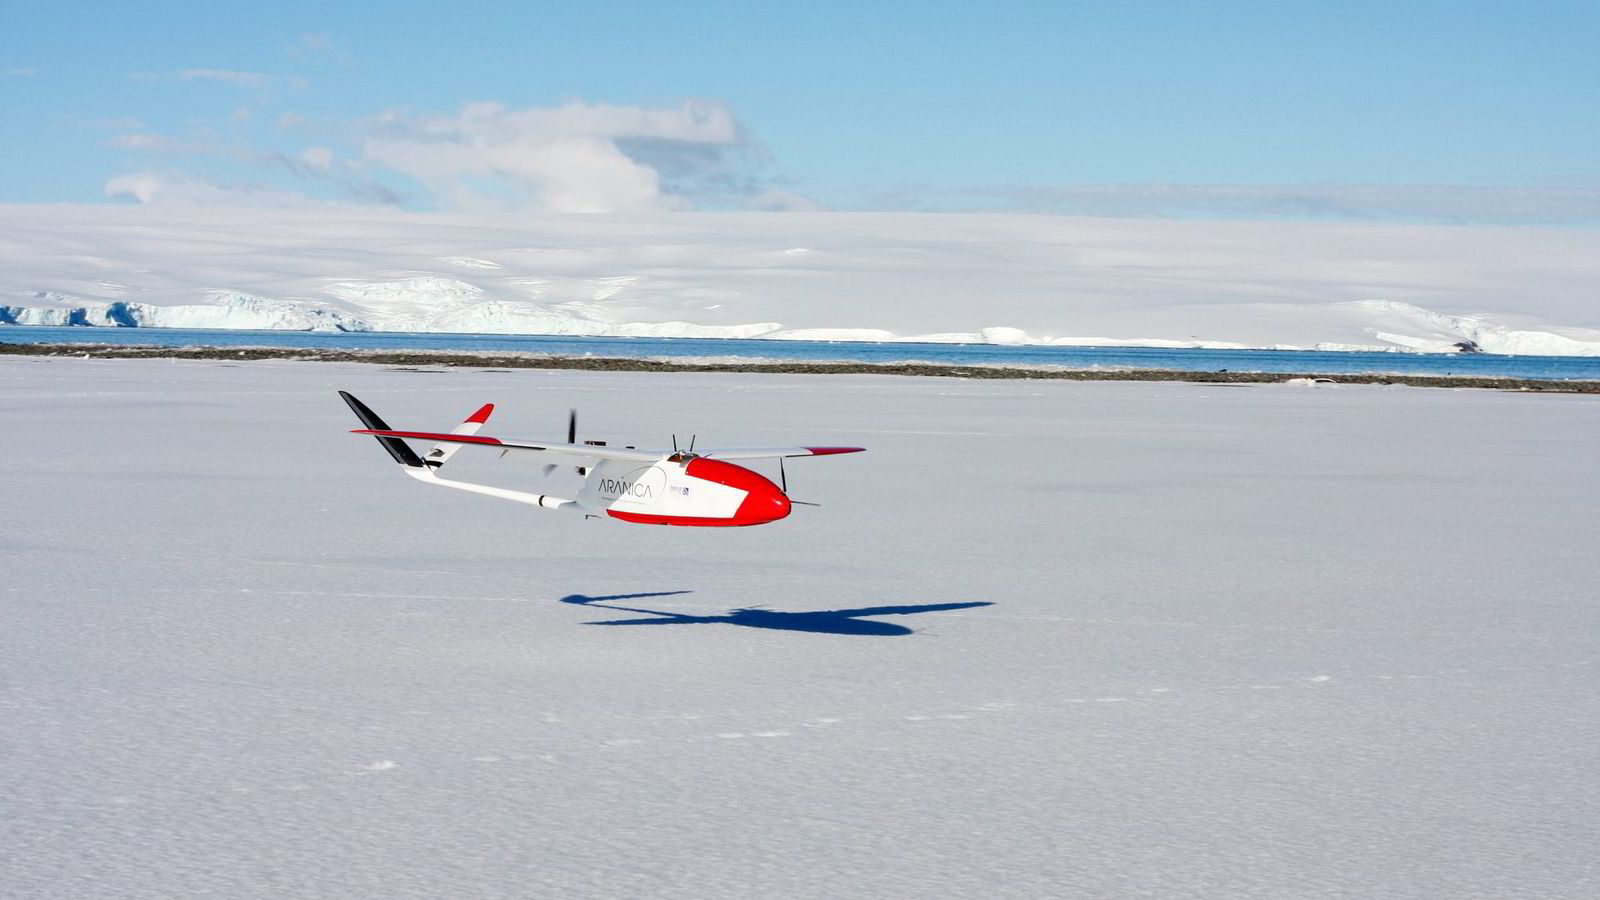
\includegraphics[width=.6\textwidth, height=9cm]{bilder/CryoWing_Explorer.jpeg}
	\caption[CryoWing Explorer]{CryoWing Explorer [2]. Noruts største fixed-wing for øyeblikket. Den brukes for større oppdrag der luftfartøyet må dekke større avstander. Den benytter også bensinmotor, og har en kropp av glassfiber, noe som gjør det mulig å kunne ha tyngre utstyr på dronen.}
\end{figure}

\begin{figure}[h!]
	\centering
	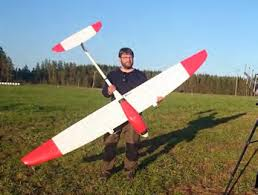
\includegraphics[width=.6\textwidth, height=9cm]{bilder/CryoWing_Scout.jpeg}
	\caption{CryoWing Scout [3]}
\end{figure}

\newpage

\begin{figure}[hpbt]
	\centering
	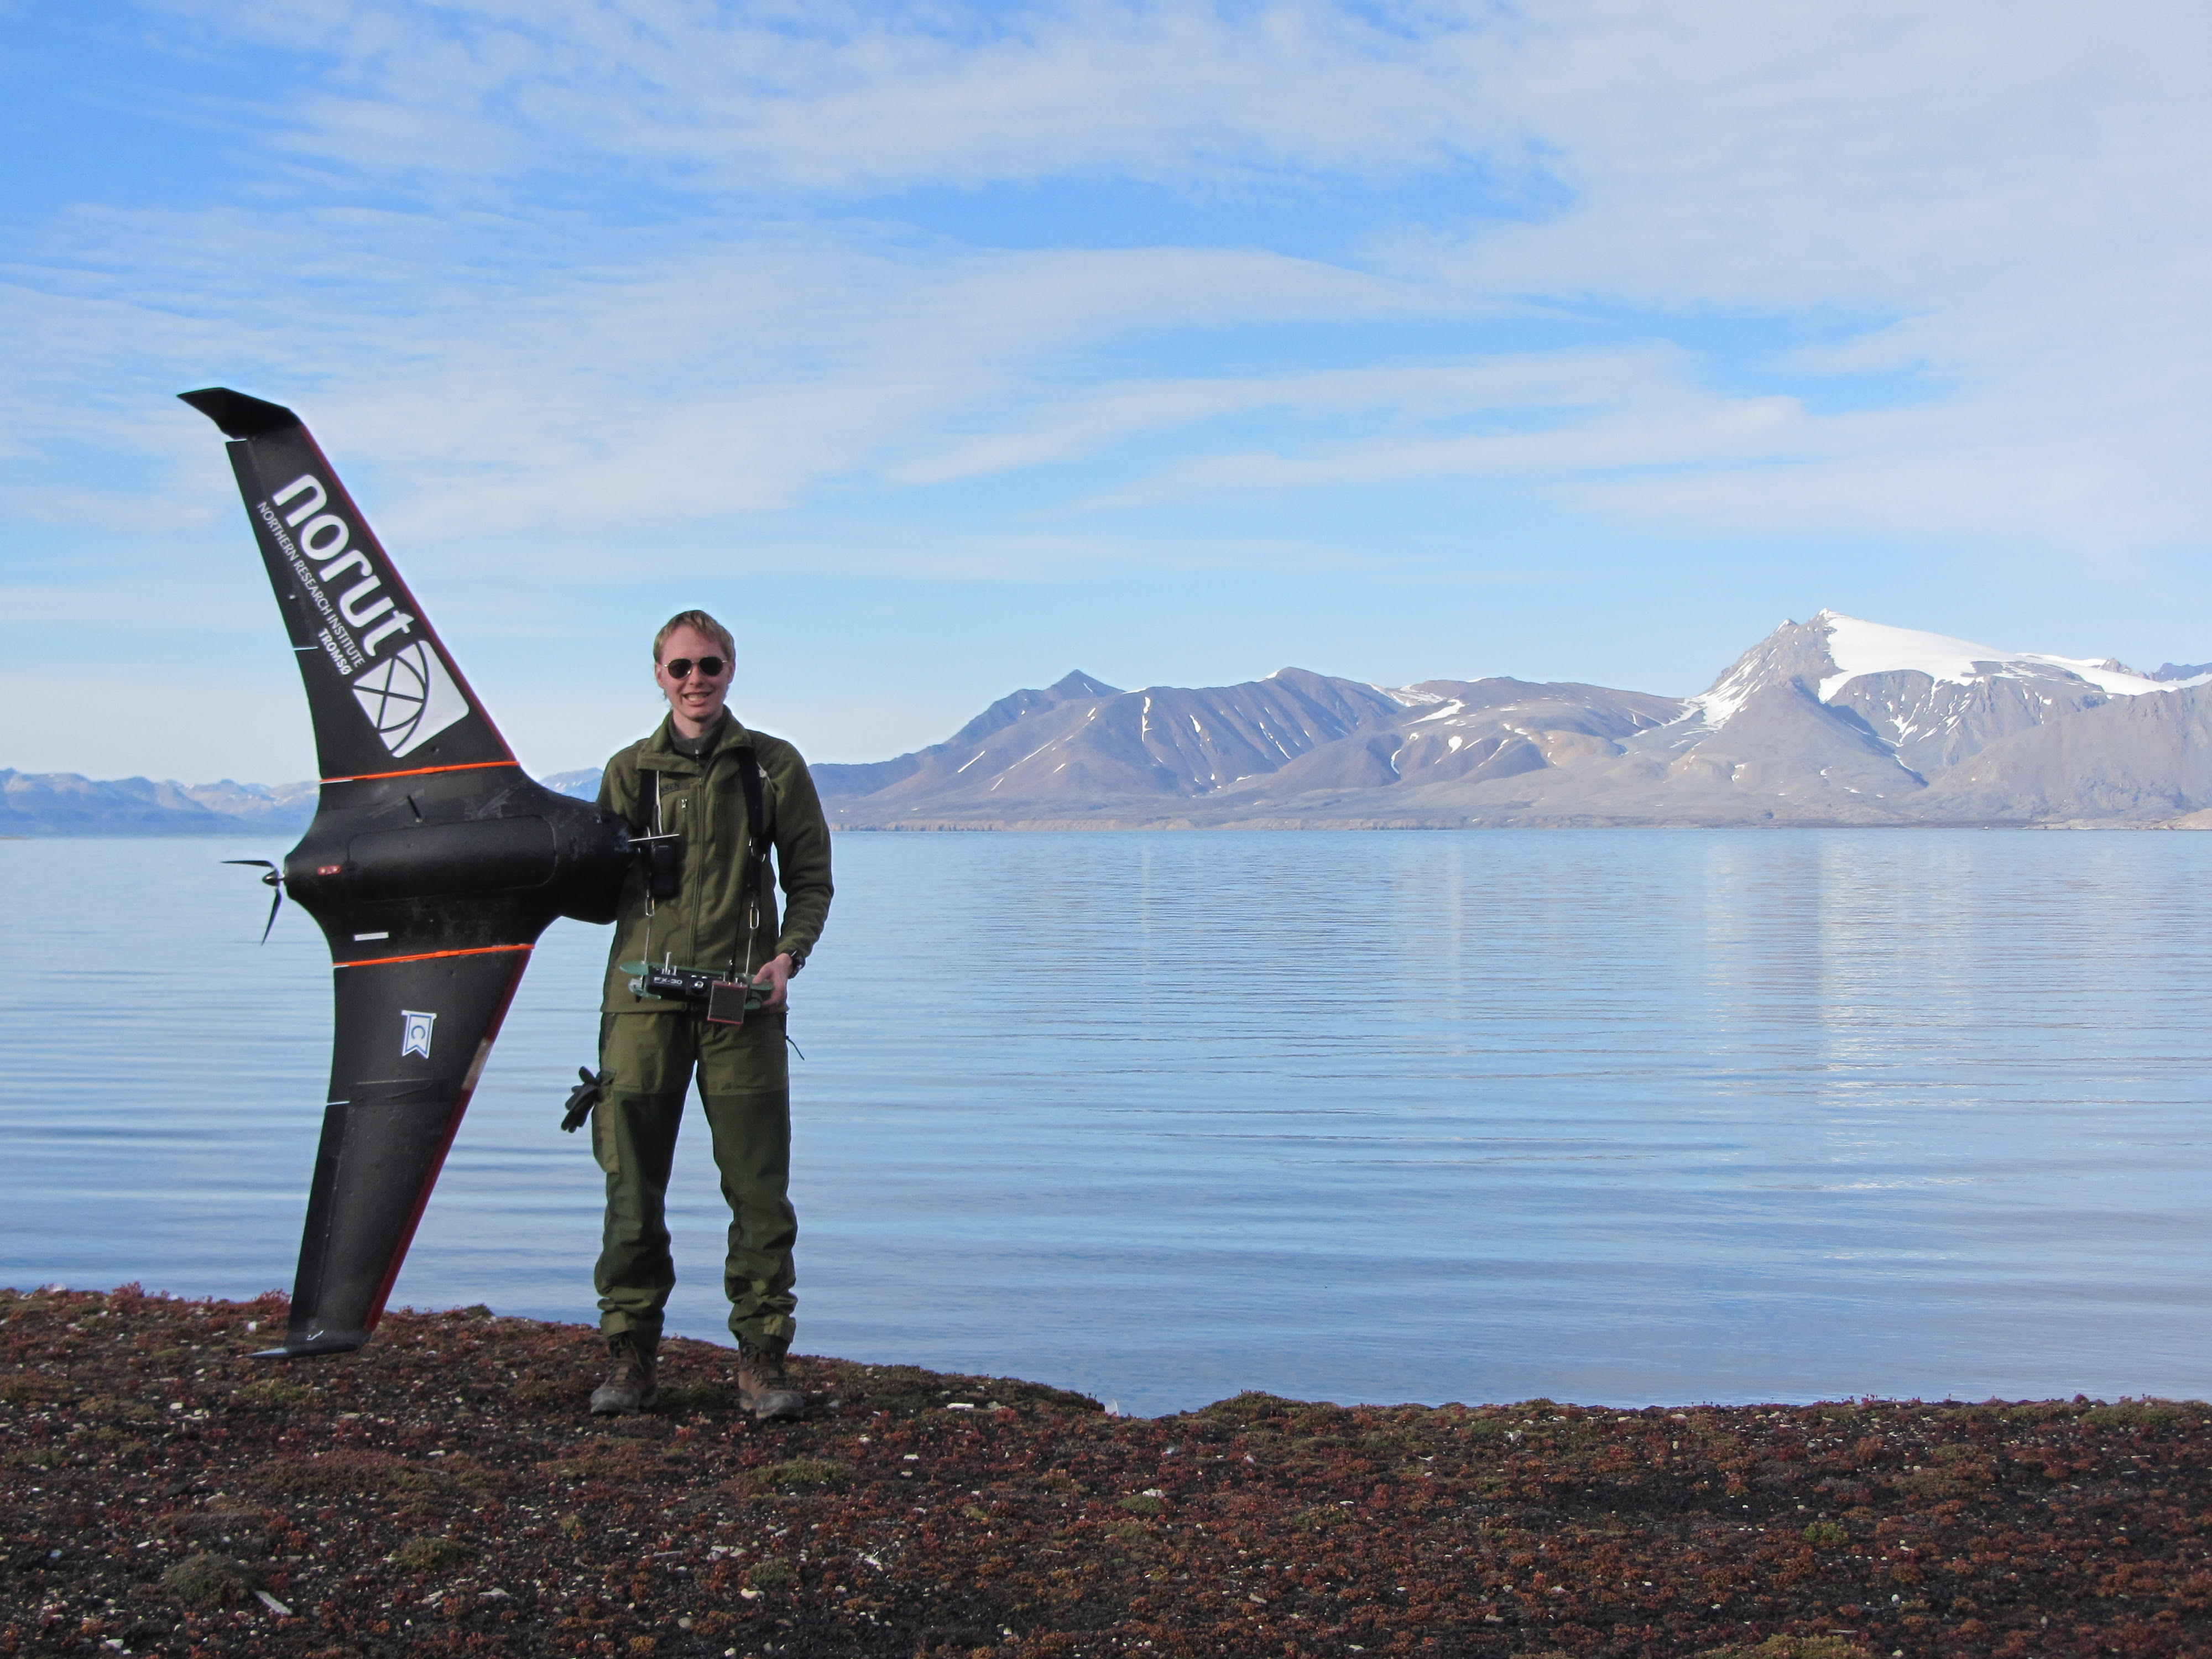
\includegraphics[width=.6\textwidth, height=9cm]{bilder/SkyWalker_X8.jpg}
	\caption{SkyWalker X8 [4]}
\end{figure}

\begin{figure}[ht]
	\centering
	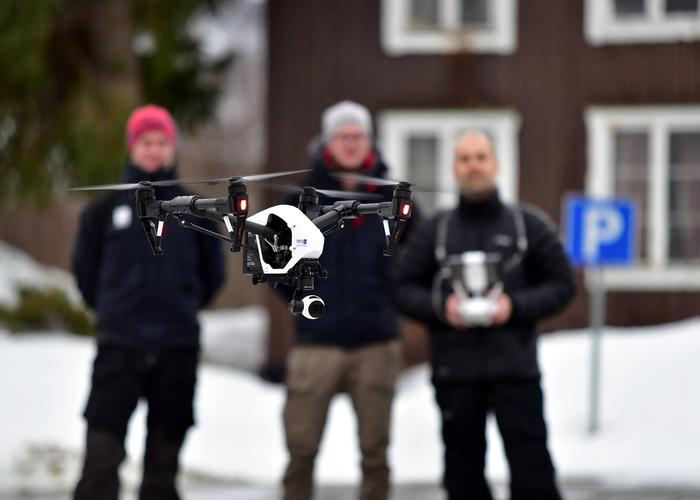
\includegraphics[width = .6\textwidth, height = 9cm]{bilder/Dji_inspire.jpg}
	\caption[DJI Inspire]{DJI Inspire [5]. Bruk av multirotorer åpner for muligheten å gjennomføre oppdrag der finere presisjon på produktet er nødvendig. Ved linjeinspeksjoner er det nødvendig at piloten kan fly nært til masten. Multirotorer gjør dette enkelt.}
\end{figure}


\clearpage
\section{Gjennomføring av praksis}
\subsection{Første uke og prosjekt}
\subsubsection{Backlog og GIS}

Den første dagen begynte med omvisning på bedriften og jeg fikk hilse på de andre som var tilstede. Deretter ble jeg satt rett i arbeid med backlog av tidligere flight plan inn i det GIS-baserte loggsystemet deres. \\
Typisk metodikk innen luftfart synes å være ``learning by doing''. Poenget er det å prøve ut for seg selv og ta utgangspunkt i eksempler som er gitt. Jeg så dermed på tidligere logger som var ført og fulgte deres oppsett.\\
En flight log er et skjema som beskriver en flyoperasjon. Loggen skal minimum inneholde flytype, tidspunkt for take-off, landing, tid i lufta, drivstoff brukt, hvilke luftfartsinstanser man har vært i kontakt med om noe, vær og så videre. 

%Bilde av loggskjema
\begin{figure}[ht]
	\centering
	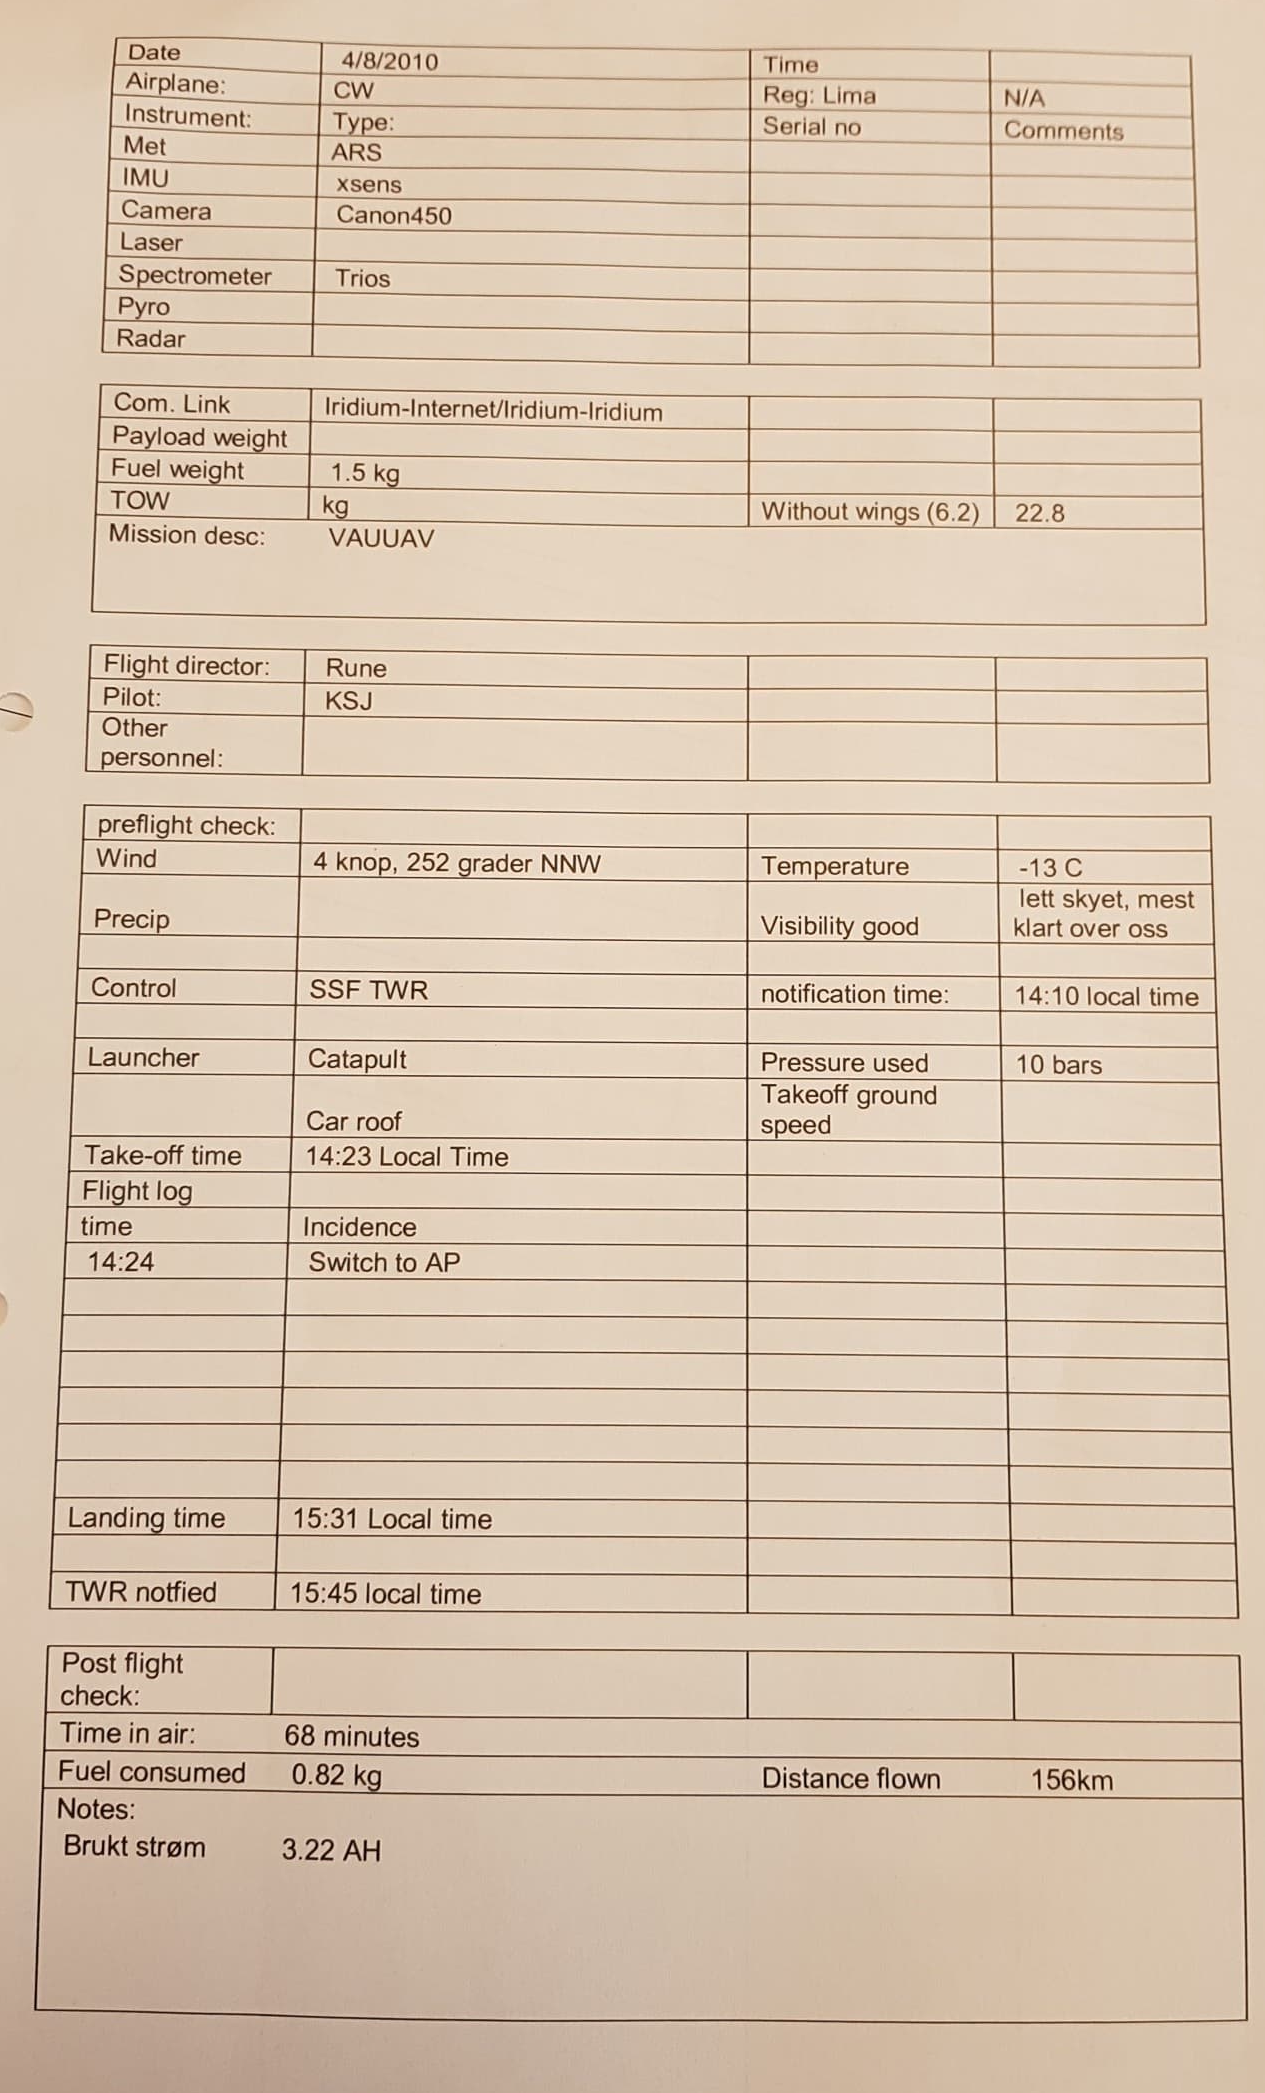
\includegraphics[height= 10cm, width=0.5\textwidth]{bilder/flightlogNorut.png}
		\caption[Loggskjema]{Typisk opplegg av loggskjema til Norut. Skjemaet skal inneholde nødvendig informasjon om flighten som kan brukes til gjennomgang for neste flight. }
\end{figure}

\newpage
Mesteparten av den første dagen gikk til backlog samt at jeg fikk delta på et avdelingsmøte.\\
\subsubsection{Forberedelse til byggeprosjekt}
Dag 2 fikk jeg et prosjekt utdelt som jeg skulle fokusere på i de neste ukene. Prosjektet gikk ut på bygging og testflyvning av tre fly av typen Cryowing Observer. \\
Flyene skulle også dokumenteres luftdyktigheten på. Det vil si at det må dokumenteres hvor god stand disse er til å følge kravene Norut har satt for sikker flyvning. Til forberedelse av prosjektet ble jeg bedt om å legge opp en plan for hvordan jeg vil finne de ulike egenskapene til flyene, som skal dokumenteres i en såkalt POH (Pilot's Operating Handbook). I denne POH'en skulle jeg blant annet finne følgende opplysninger gjennom testflygninger: 
\begin{itemize}
	\item Cruise speed: Flyets hastighet ved konstant høyde
	\item Stall speed: Flyets minimale hastighet før det ikke opprettholder løft
	\begin{itemize}
		\item Flap up power off
		\item Half flap power off
		\item Full flap power off	
	\end{itemize}
	\item Standard empty weight: Flyets vekt uten nyttelast og batteri
	\item Maximal Take Off Weight (MTOW): Flyets maksimale vekt
	\item Useful load: Total vekt av nyttelast og batteri
	\item Wing loading: Forholdet mellom flyets vekt og vingearealet
	\item Power loading: Forholdet mellom flyets vekt og motorens effekt
	\item Minimal battery capacity: Minimal batteristørrelse for optimal flyging. 
\end{itemize}
Oppsettet jeg lagde for testflygningen er vedlagt til rapporten, se vedlegg nr. 6. 
Selve byggingen av luftfartøyene kunne ikke begynne før uke 2, da delene måtte hentes opp fra Bodø. \\ 
\newpage
I mellomtiden drev jeg med reparasjonsarbeid på et av Noruts multirotorer som havarerte. Nye rammer måtte settes på, elektroniske fartskontrollere måtte kobles opp og konfigureres og mer. Da jeg har drevet med noe bygging av multirotorer fra hobbybasis, samt fått teoretisk kompetanse innenfor elektronikk fra studiet, gikk mye av arbeidet bra. Konfigurasjonene som Norut bruker (se bildene under), var litt nytt, men prinsippet var det samme som på hobbyprosjektene mine. \\

\begin{figure}[ht]
	\centering
	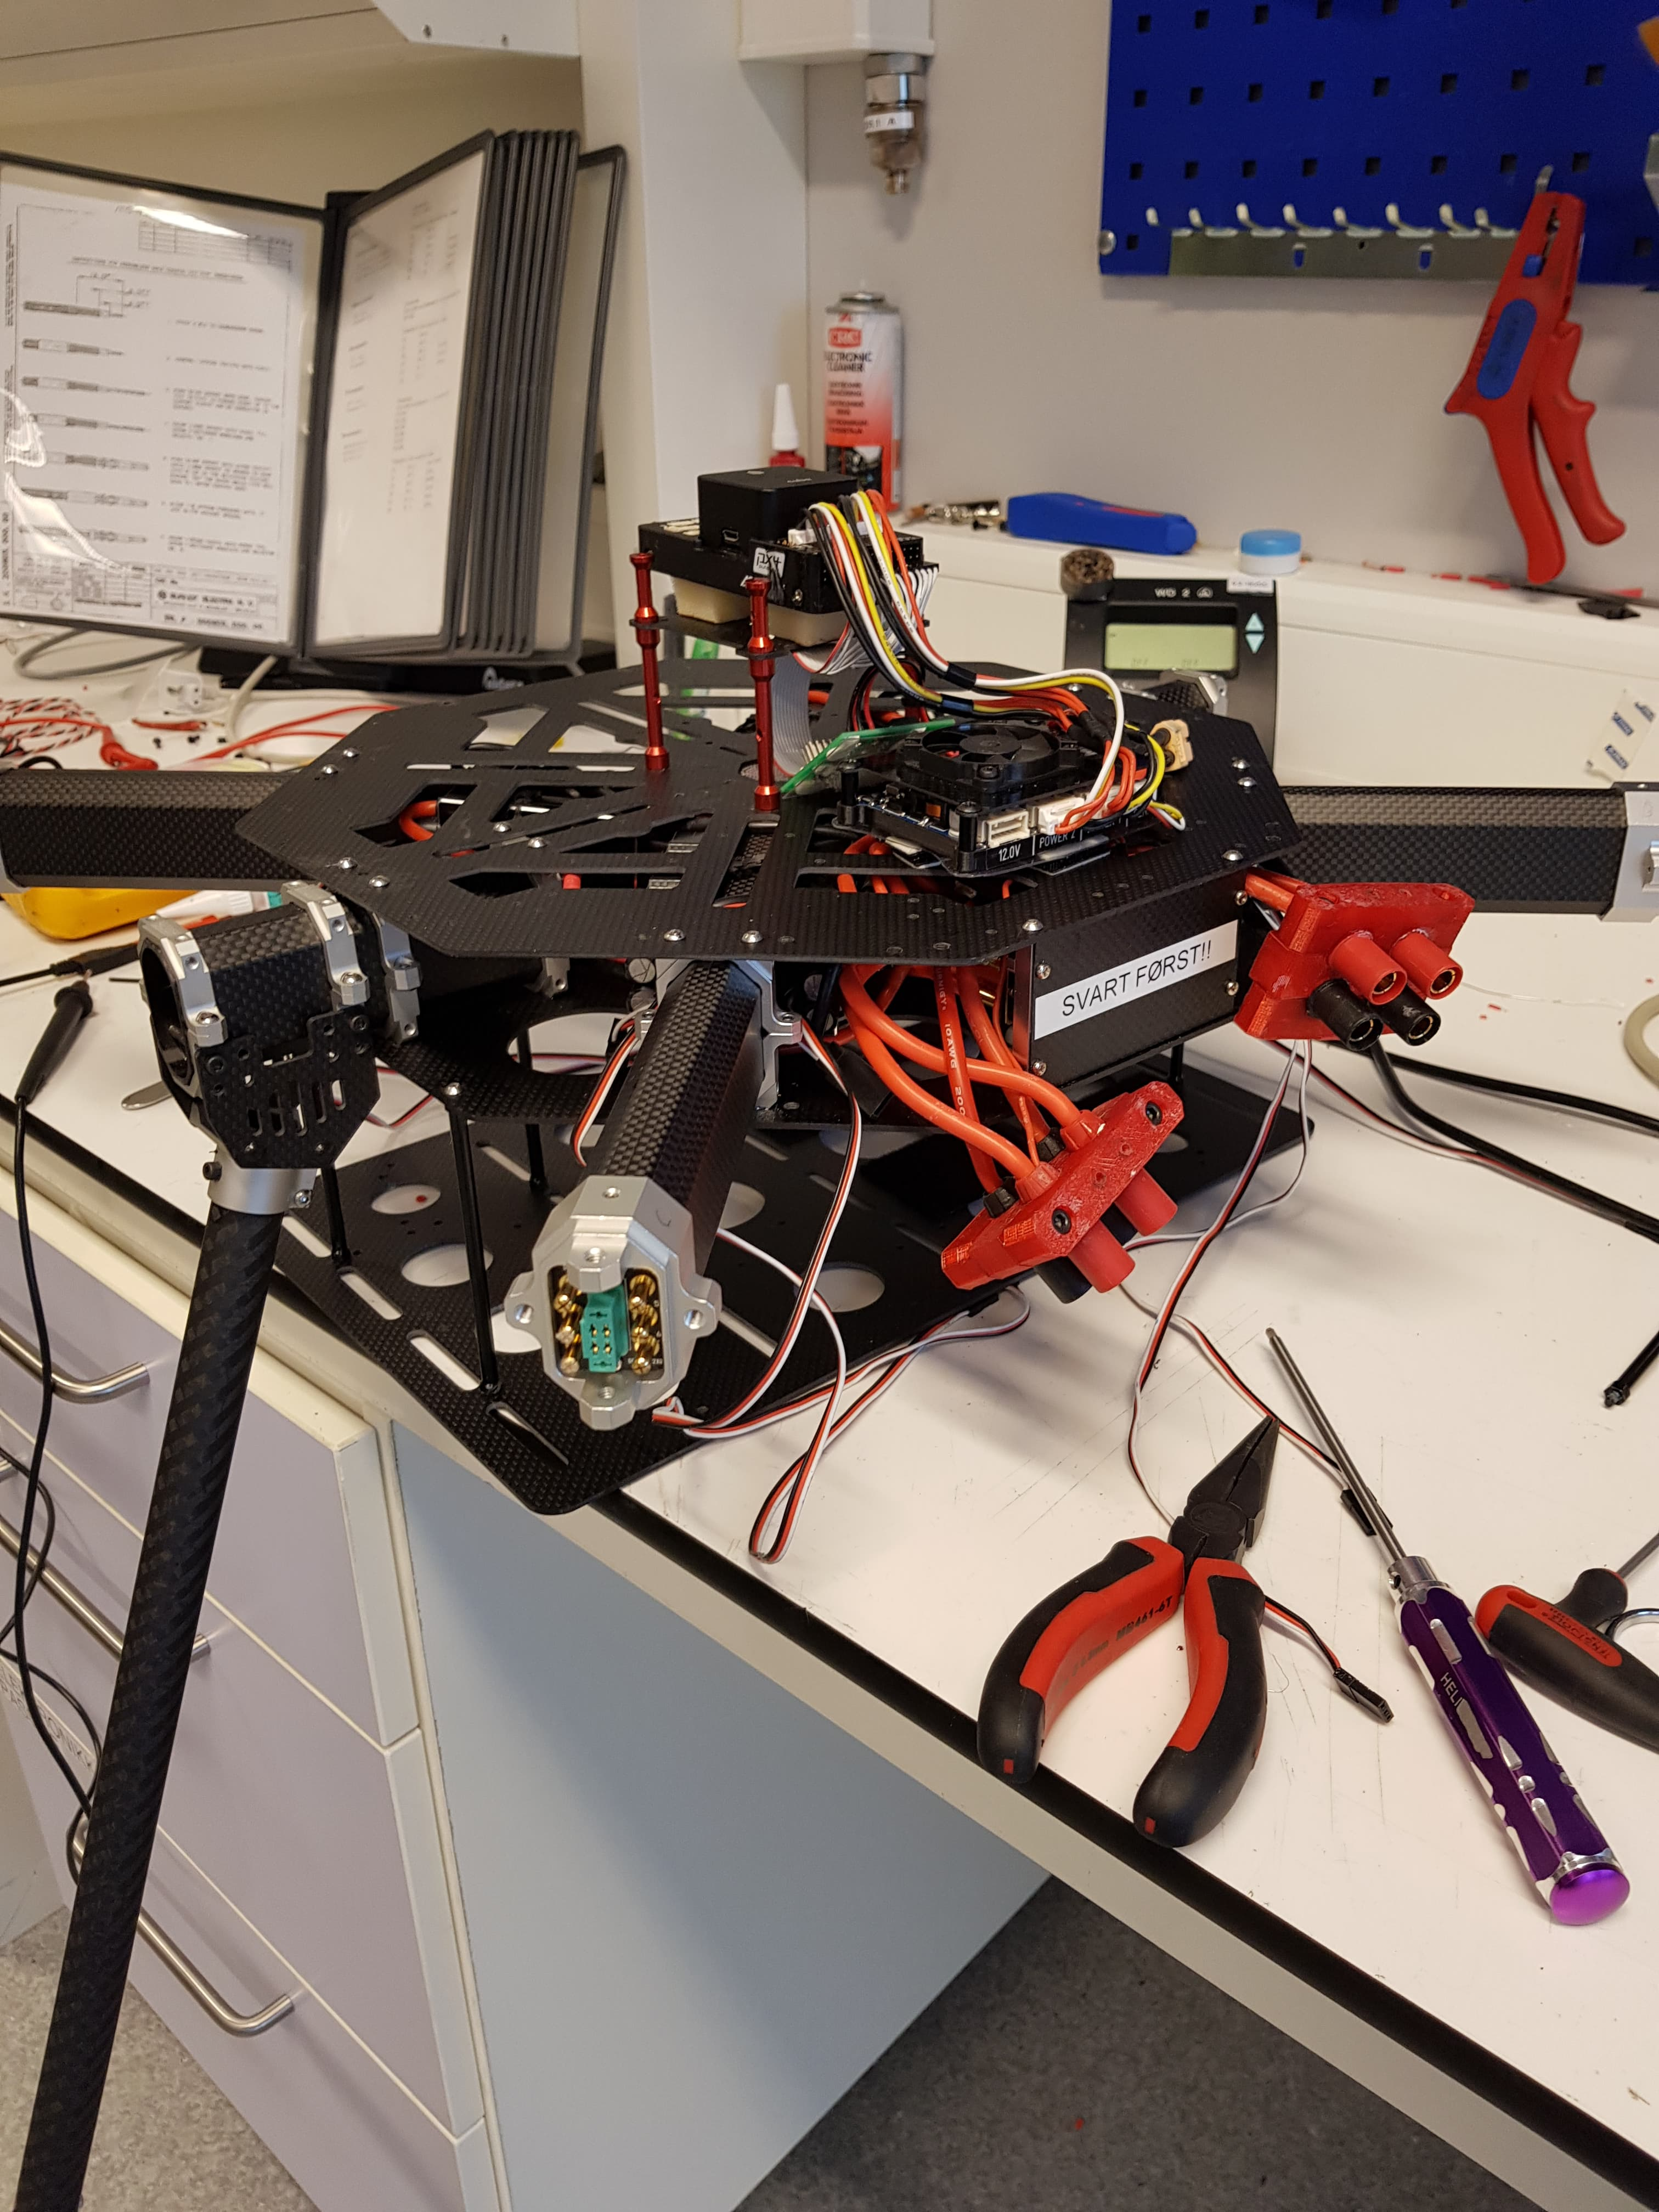
\includegraphics[height = 8cm, width = 0.6\textwidth]{bilder/octocopt_x8.jpg}
	\caption[Reparasjonsarbeid]{Reparasjonsarbeid på en octocopter i såkalt X8 - konfigurasjon.}
\end{figure}
%Teknisk prosjekt - Cryowing Observer
%\newpage
\begin{figure}[ht]
	\centering
	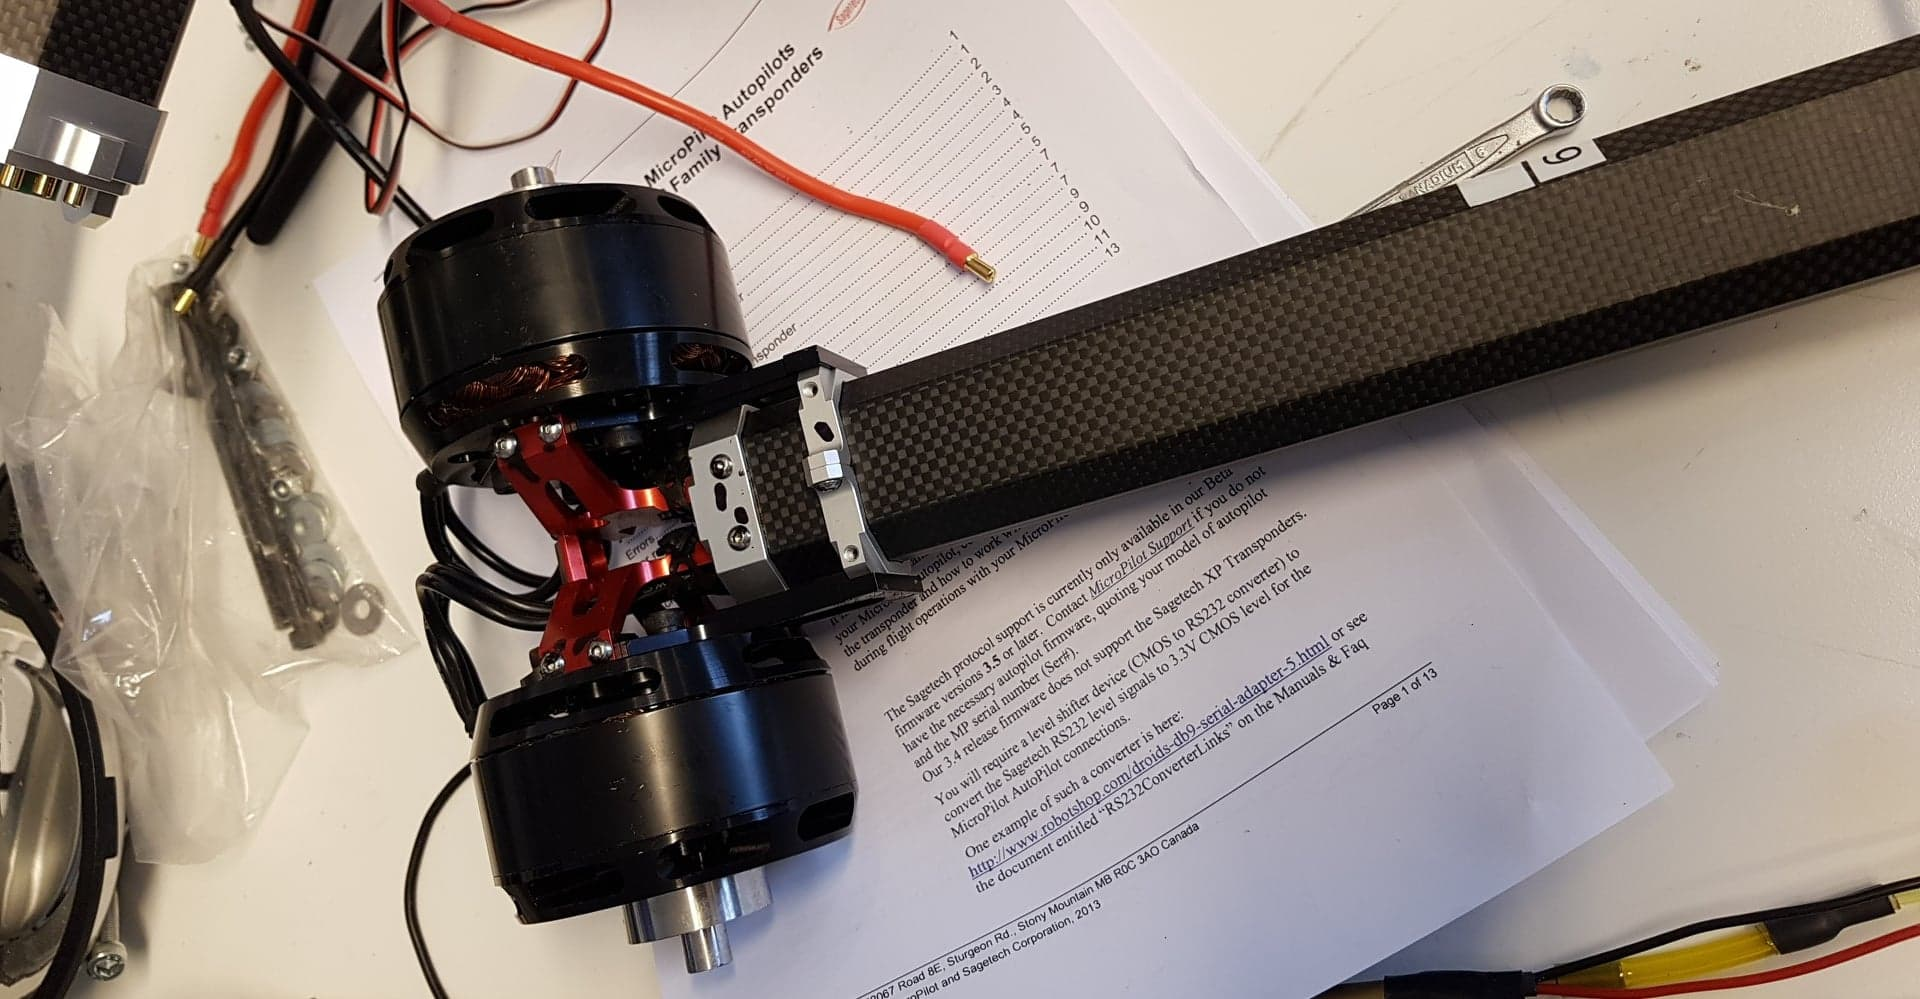
\includegraphics[scale=.2]{bilder/octarm_x8.jpg}
	\caption[Motormontering]{Montering av nye motorer på ytre armer.}
\end{figure}

\subsection{Påfølgende uker: Byggeprosjekt}
\subsubsection{Montering}
Da jeg endelig fikk delene til Cryowing Observer - fartøyene, kunne jeg begynne prosjektet. Hele denne uken og neste uke gikk til bygging av første flykropp. Dette tok lang tid da det var lite med ressurser og folk til hjelp for å kunne få flyet ferdig i løpet av første prosjektuke. Ikke alle delene fra Bodø ble hentet opp, og materialene var dårlig systematisert. Det gikk mye tid i å finne riktige materialer til de ulike delene.\\
Til tross for dette var dette en fin oppgave i å få utforske og prøve ulike metoder for å komme frem til en løsning. Jeg har jobbet med multirotorer før, men montering av servoer og håndtering av EPO-materiale - også kjent som isopor - var helt nytt for meg. Det var dermed en bratt læringskurve. \\ Min plan for gjennomføring av byggeprosjektet var å sette sammen flyene med servoer, kropp, vinger og utstyrskuppel, se bildene under.

Jeg begynte med montering av vingene, ved å sette på servoer og lime kryssfinér-spanter til vingene. Servoene ble festet med enten varmlim eller lynlim. Alle servoene som settes på måtte sentreres ved hjelp av en servo-tester, slik at det blir enklest å sette opp flyet elektronisk. 

\begin{figure}[ht]
	\centering
	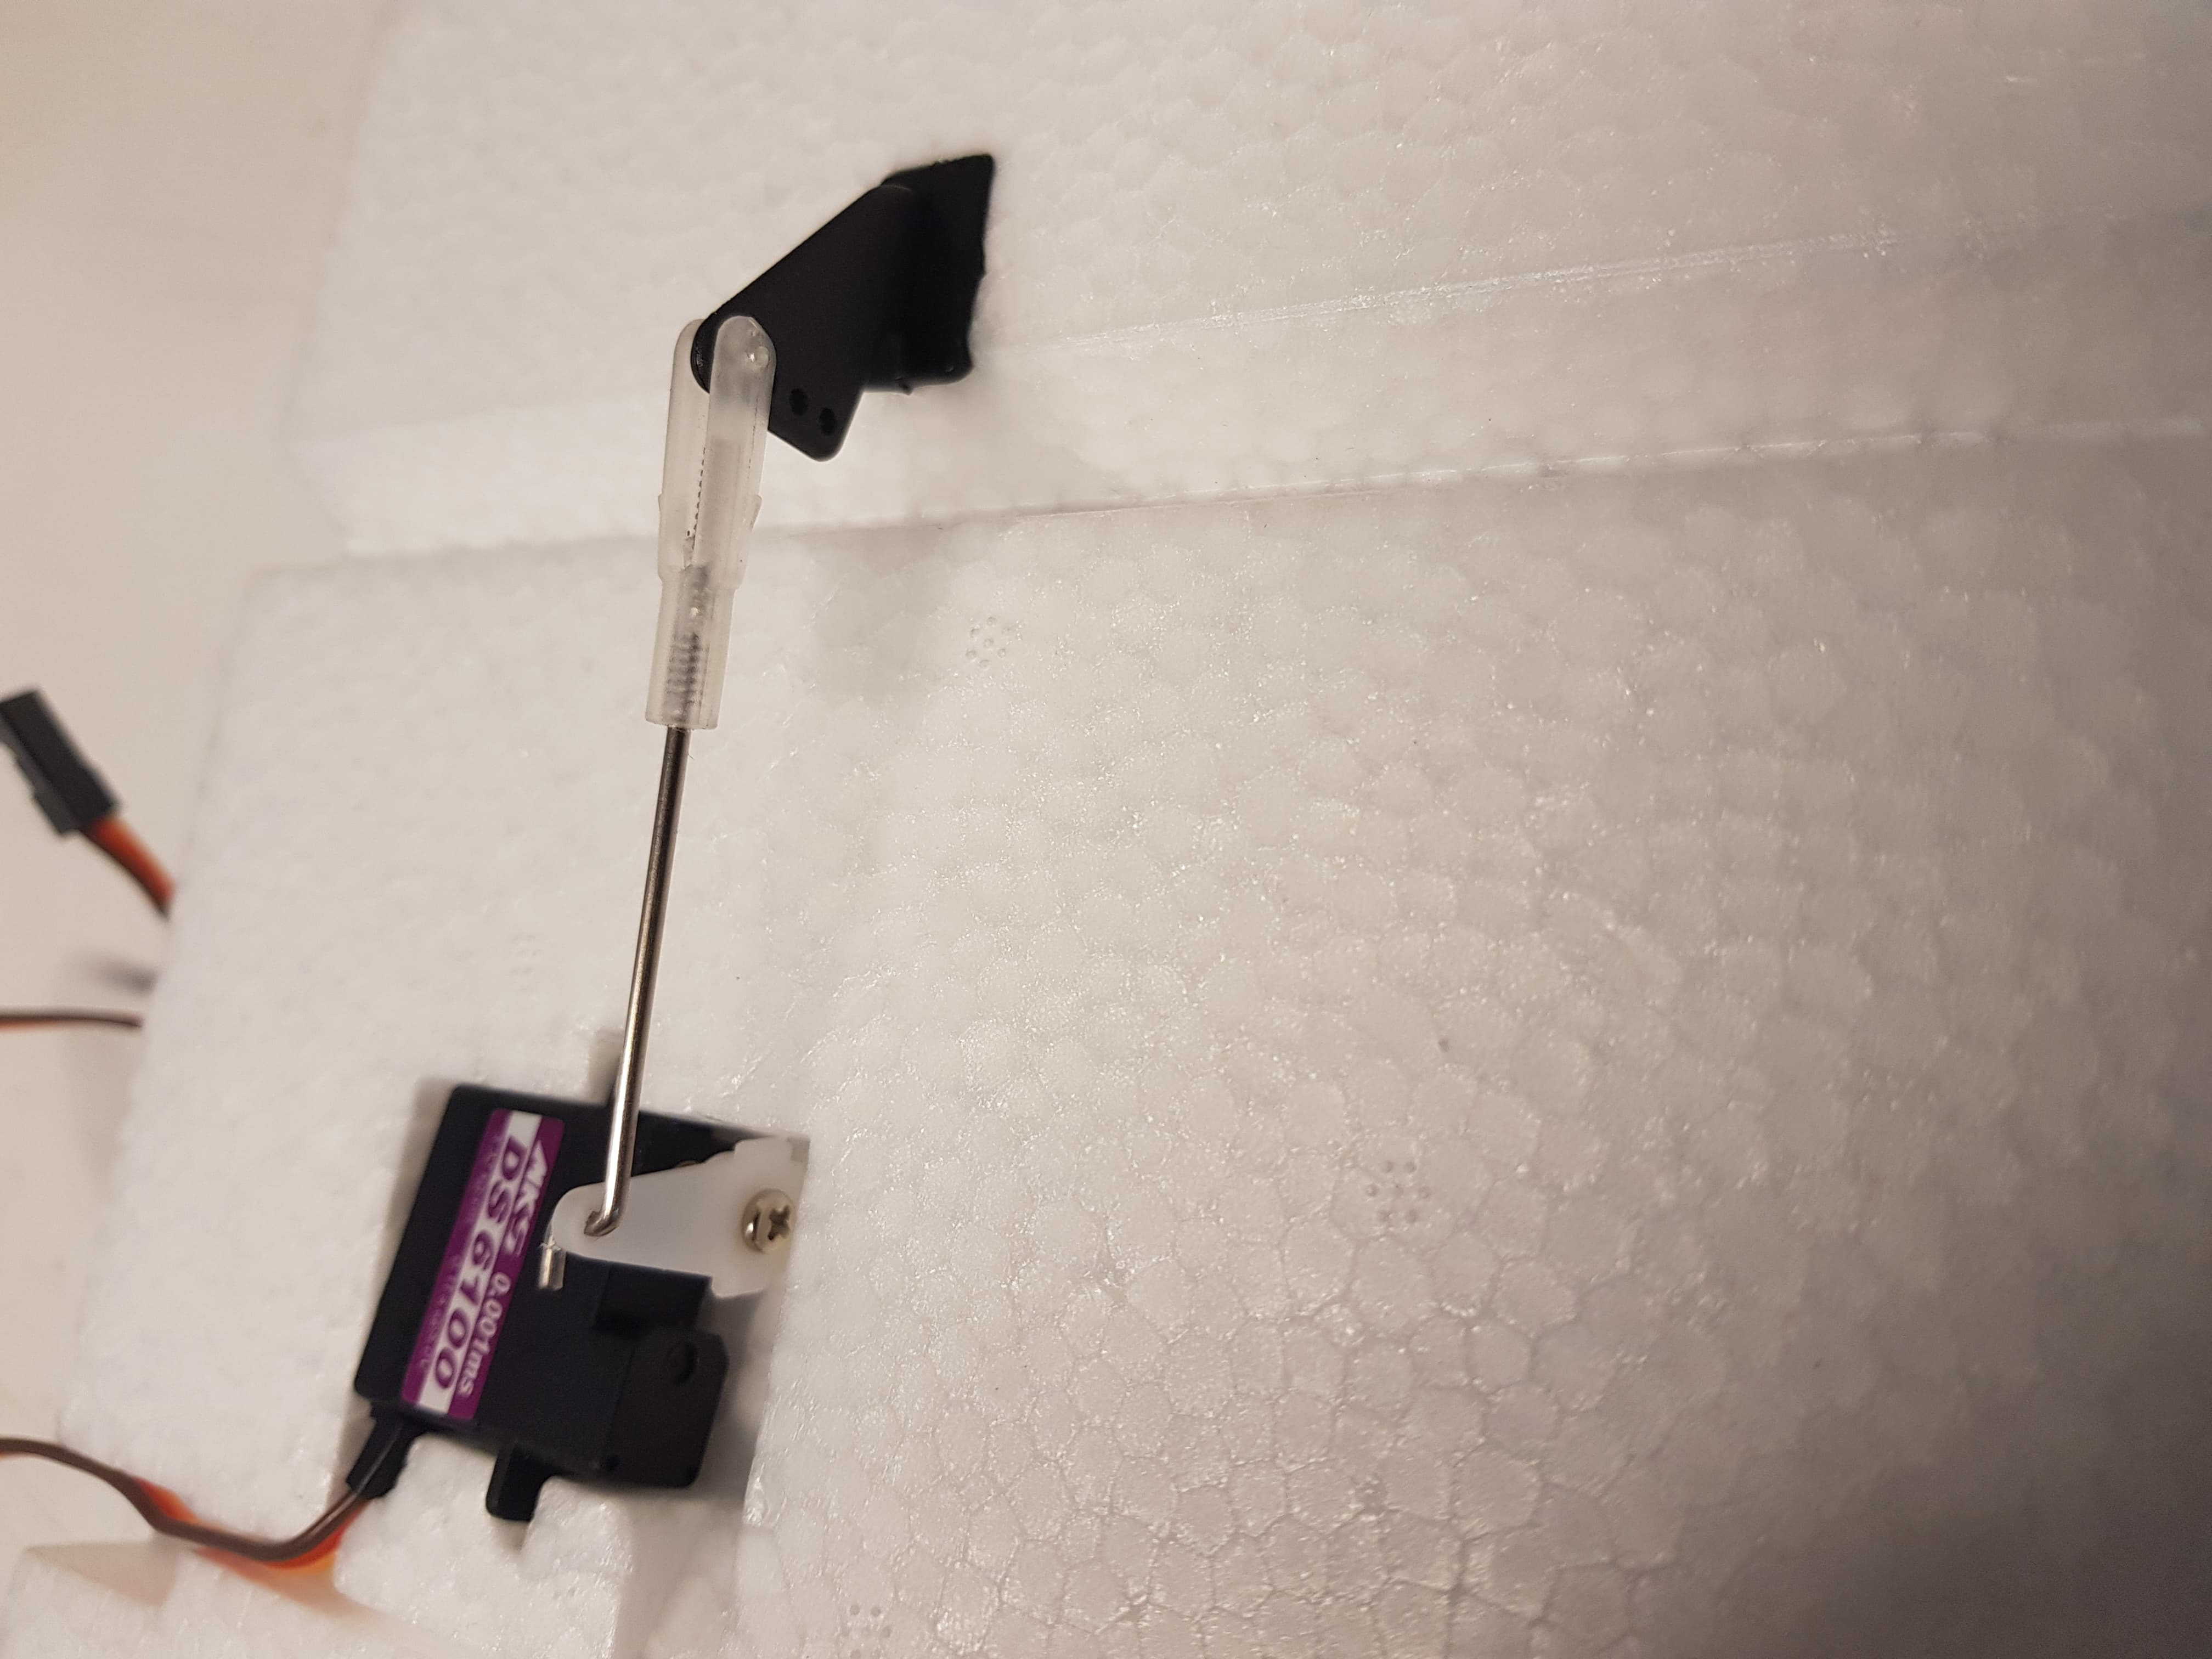
\includegraphics[height = 10cm, width = .6\textwidth]{bilder/servomontering.jpg}
	\caption[Servoorientering]{Riktig montering av servo, der servohornet er \ang{90} med horisontalplanet (her vingen).}
\end{figure}

\begin{figure}[ht]
	\centering
	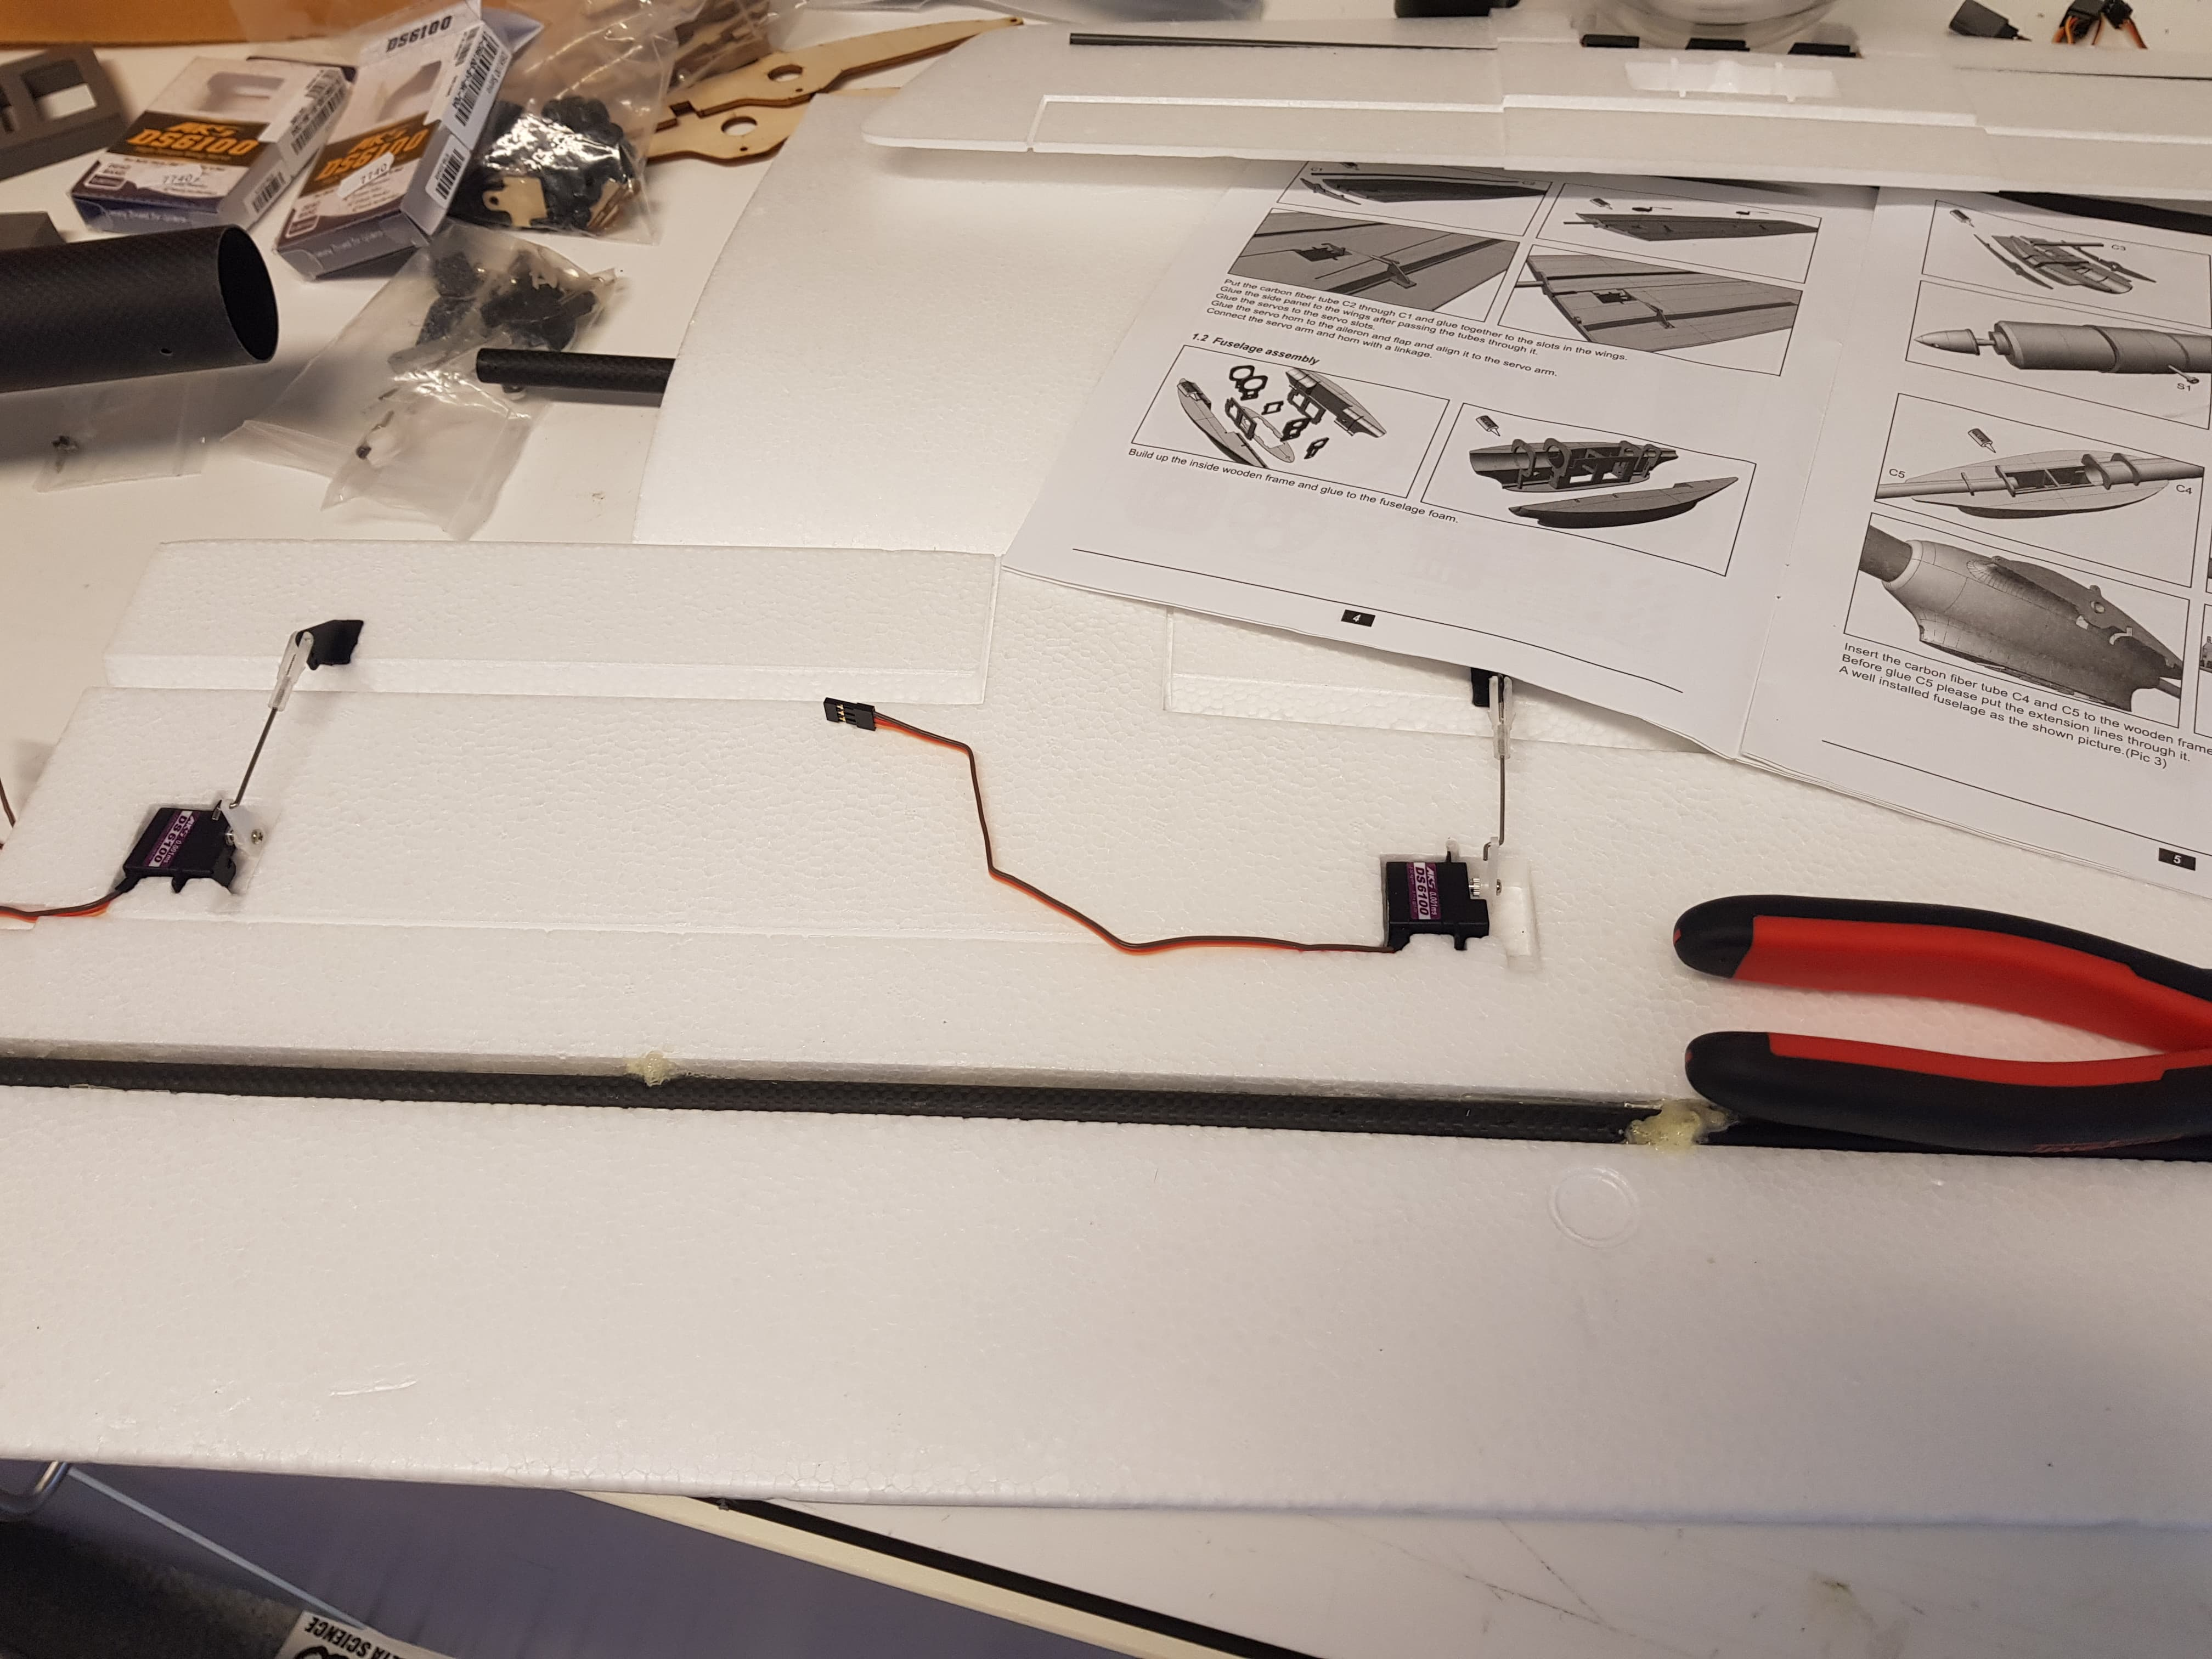
\includegraphics[width=.6\textwidth,  height = 8cm]{bilder/vingemontering.jpg}
	\caption{Montering av vinger}
\end{figure}

\newpage
Deretter gikk det til montering av motor på den fremre karbonbommen. Motoren, som er av typen BLDC (børsteløs DC-motor), drives av en fartsregulator, populært kalt ESC. Denne ESC'en inneholder en spenningsregulator som tar inn batterispenningen og gir ut en lavspenningskilde som kan brukes til å forsyne mottaker og andre periferier. 

\begin{figure}[ht]
	\centering
	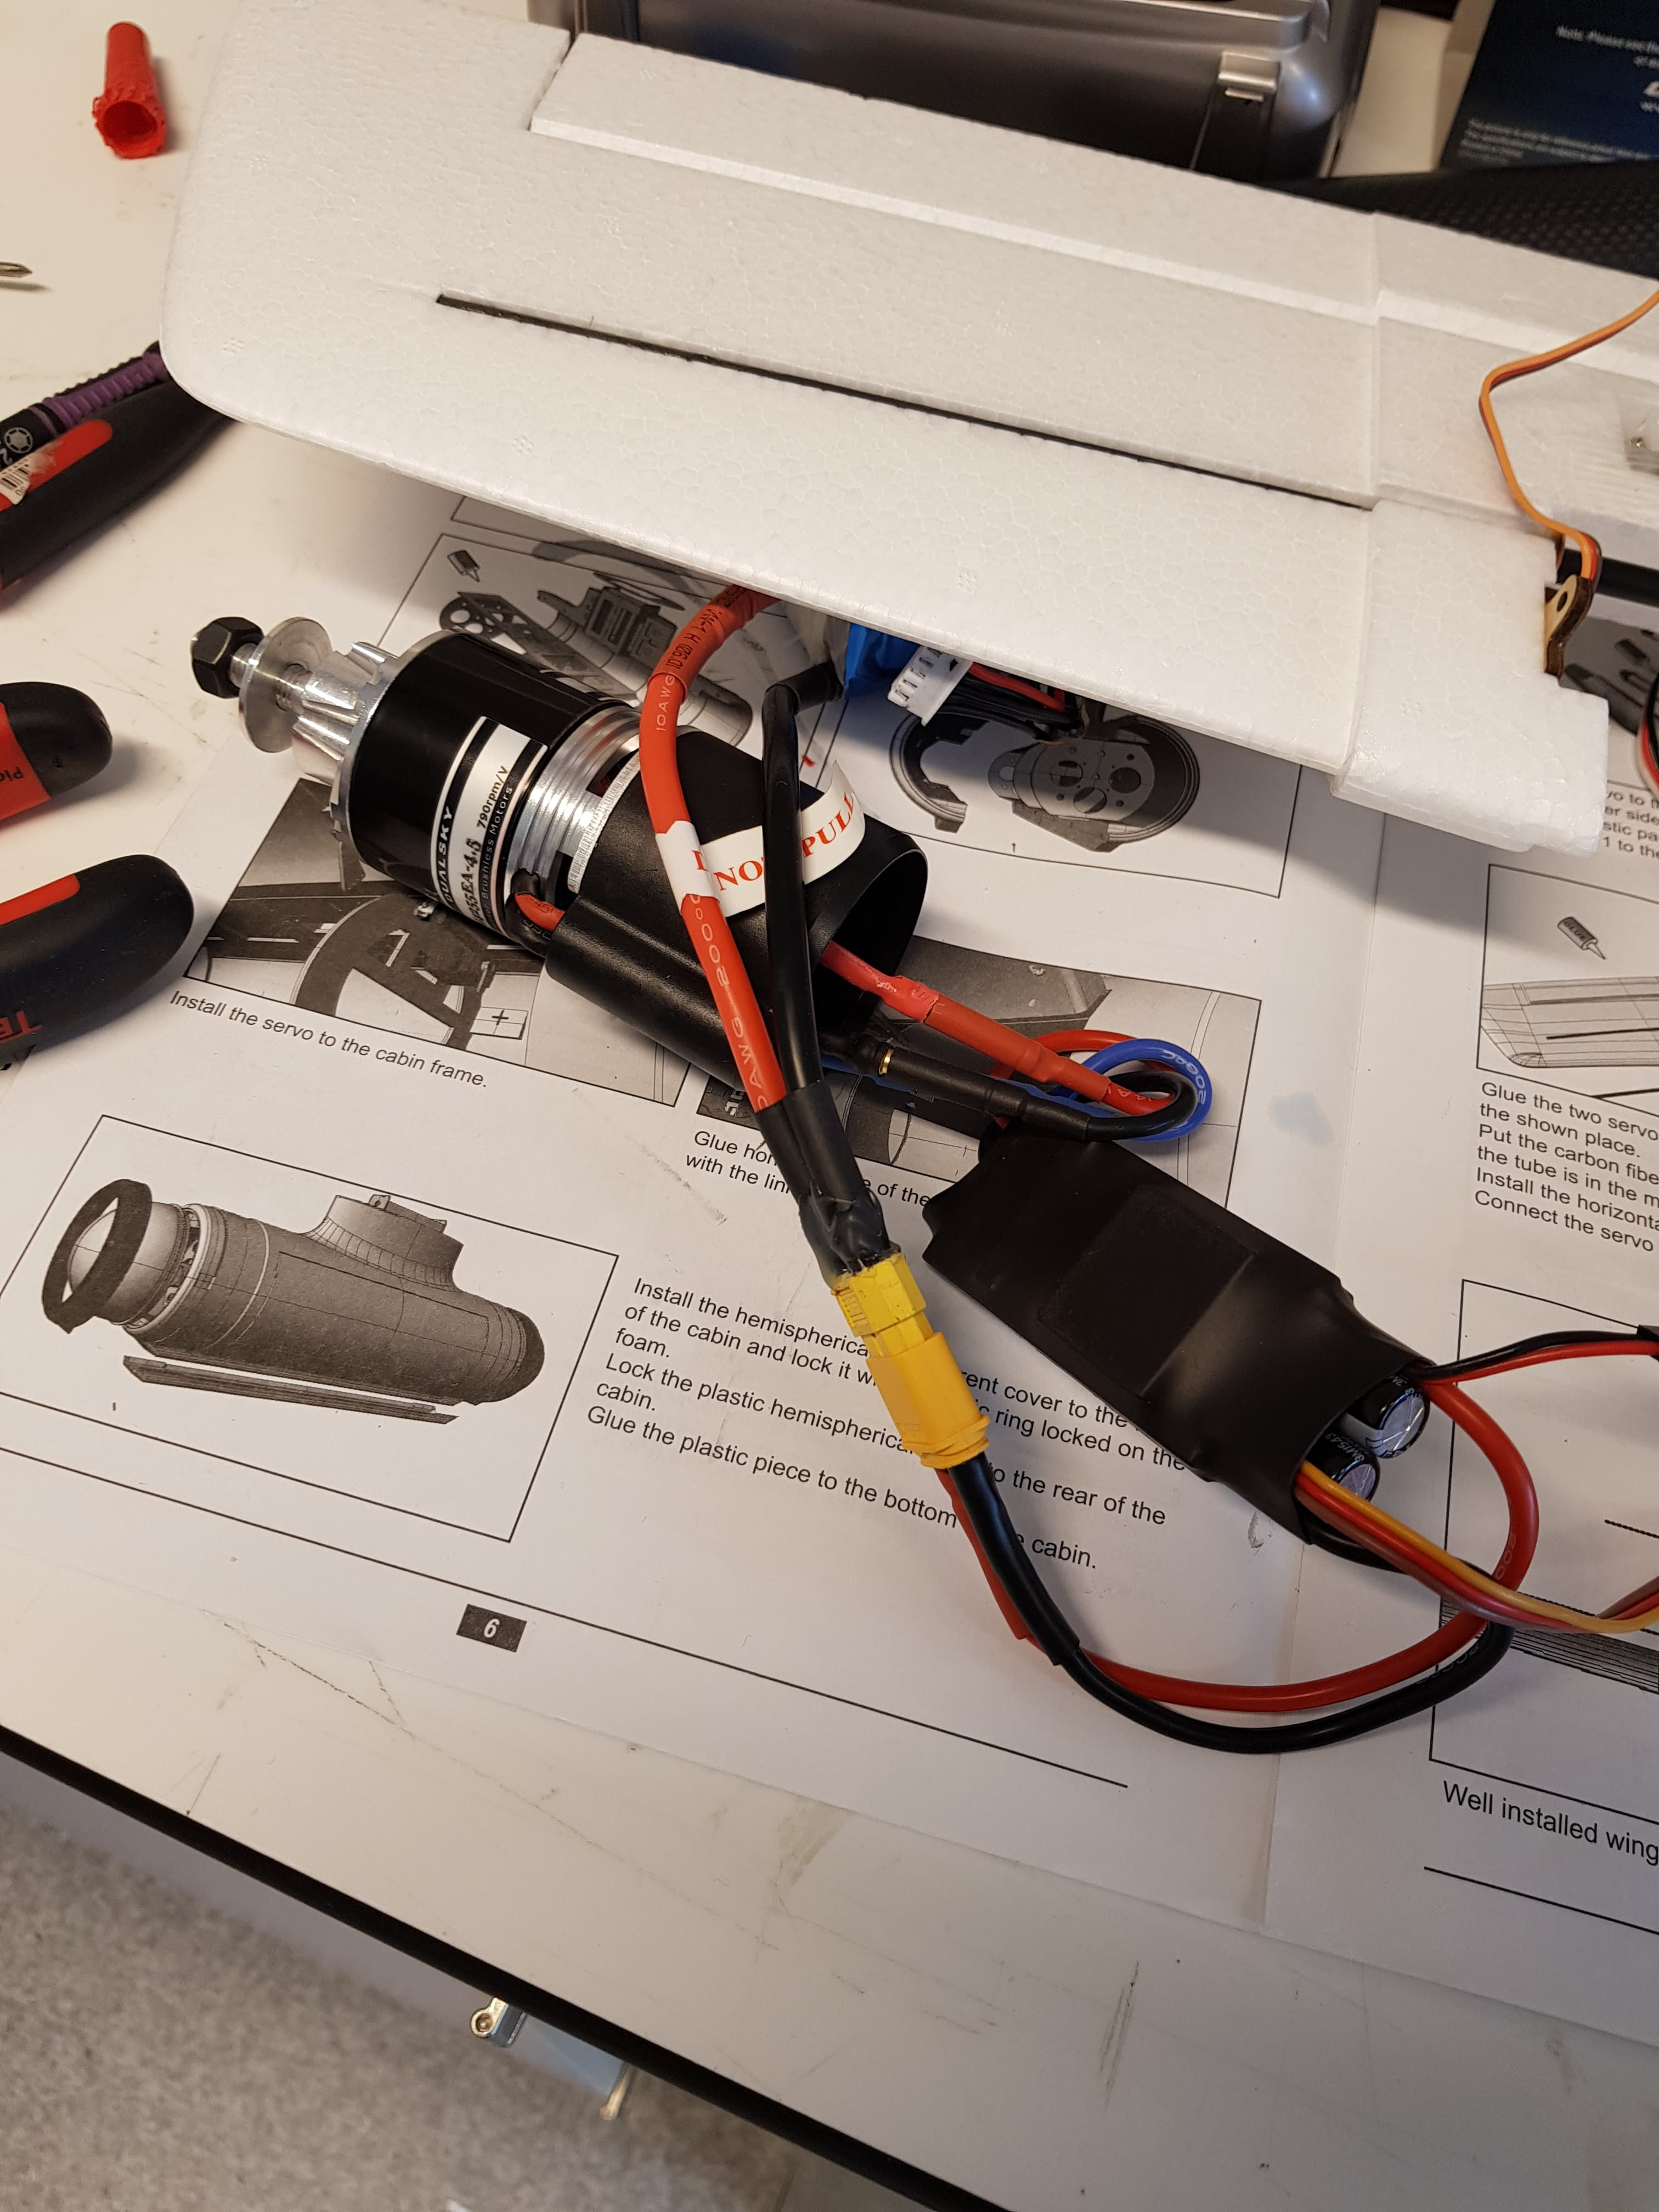
\includegraphics[height=7.6cm, width = .55\textwidth]{bilder/esc_og_motor.jpg}
	\caption[Observer-motor]{Motor tilkoblet ESC, med bryter bypassed. XT-60 - connectoren (den gule pluggen) måtte loddes på ESC-enden.}
\end{figure}

\newpage
Etter påmontert motor på karbonrøret, kunne røret limes på til undersiden av den midtre flykroppen ved hjelp av epoxy. Men på grunn av at epoxy ikke skaper en god kjemisk binding med EPO/isopor, men bare en fysisk binding, måtte jeg gjøre overflaten så stor som mulig. Jeg pusset begge overflatene med grovt sandpapir og lagde flere hull i EPO'en slik at epoxyen kan feste seg. 
Men ting gikk ikke helt som planlagt, da jeg fikk vite underveis at visse deler hadde jeg montert feil, slik som at et karbonrør var for langt inn i kroppen. Da blokkerer det bakre karbonrøret for eventuell GPS som kan monteres inni ramma. Dette førte til at jeg måtte hule ut overkroppen for at den skulle passe til underkroppen. \\
Dessuten hadde jeg aldri brukt epoxy før og visste ikke hvordan man skulle få godt nok feste mellom materialene. Første forsøk på liming ble derfor dårlig og måtte gjøres på nytt. Jeg fikk ingen veiledning på dette, bare at dette måtte gjøres om igjen. Til slutt, etter to forsøk, fikk jeg hjelp av en til å få godt nok feste. Epoxyen måtte tilsettes fyllmiddel for å kompensere for all materiale som ble skrapet av. \\


\begin{figure}[ht]
	\centering
	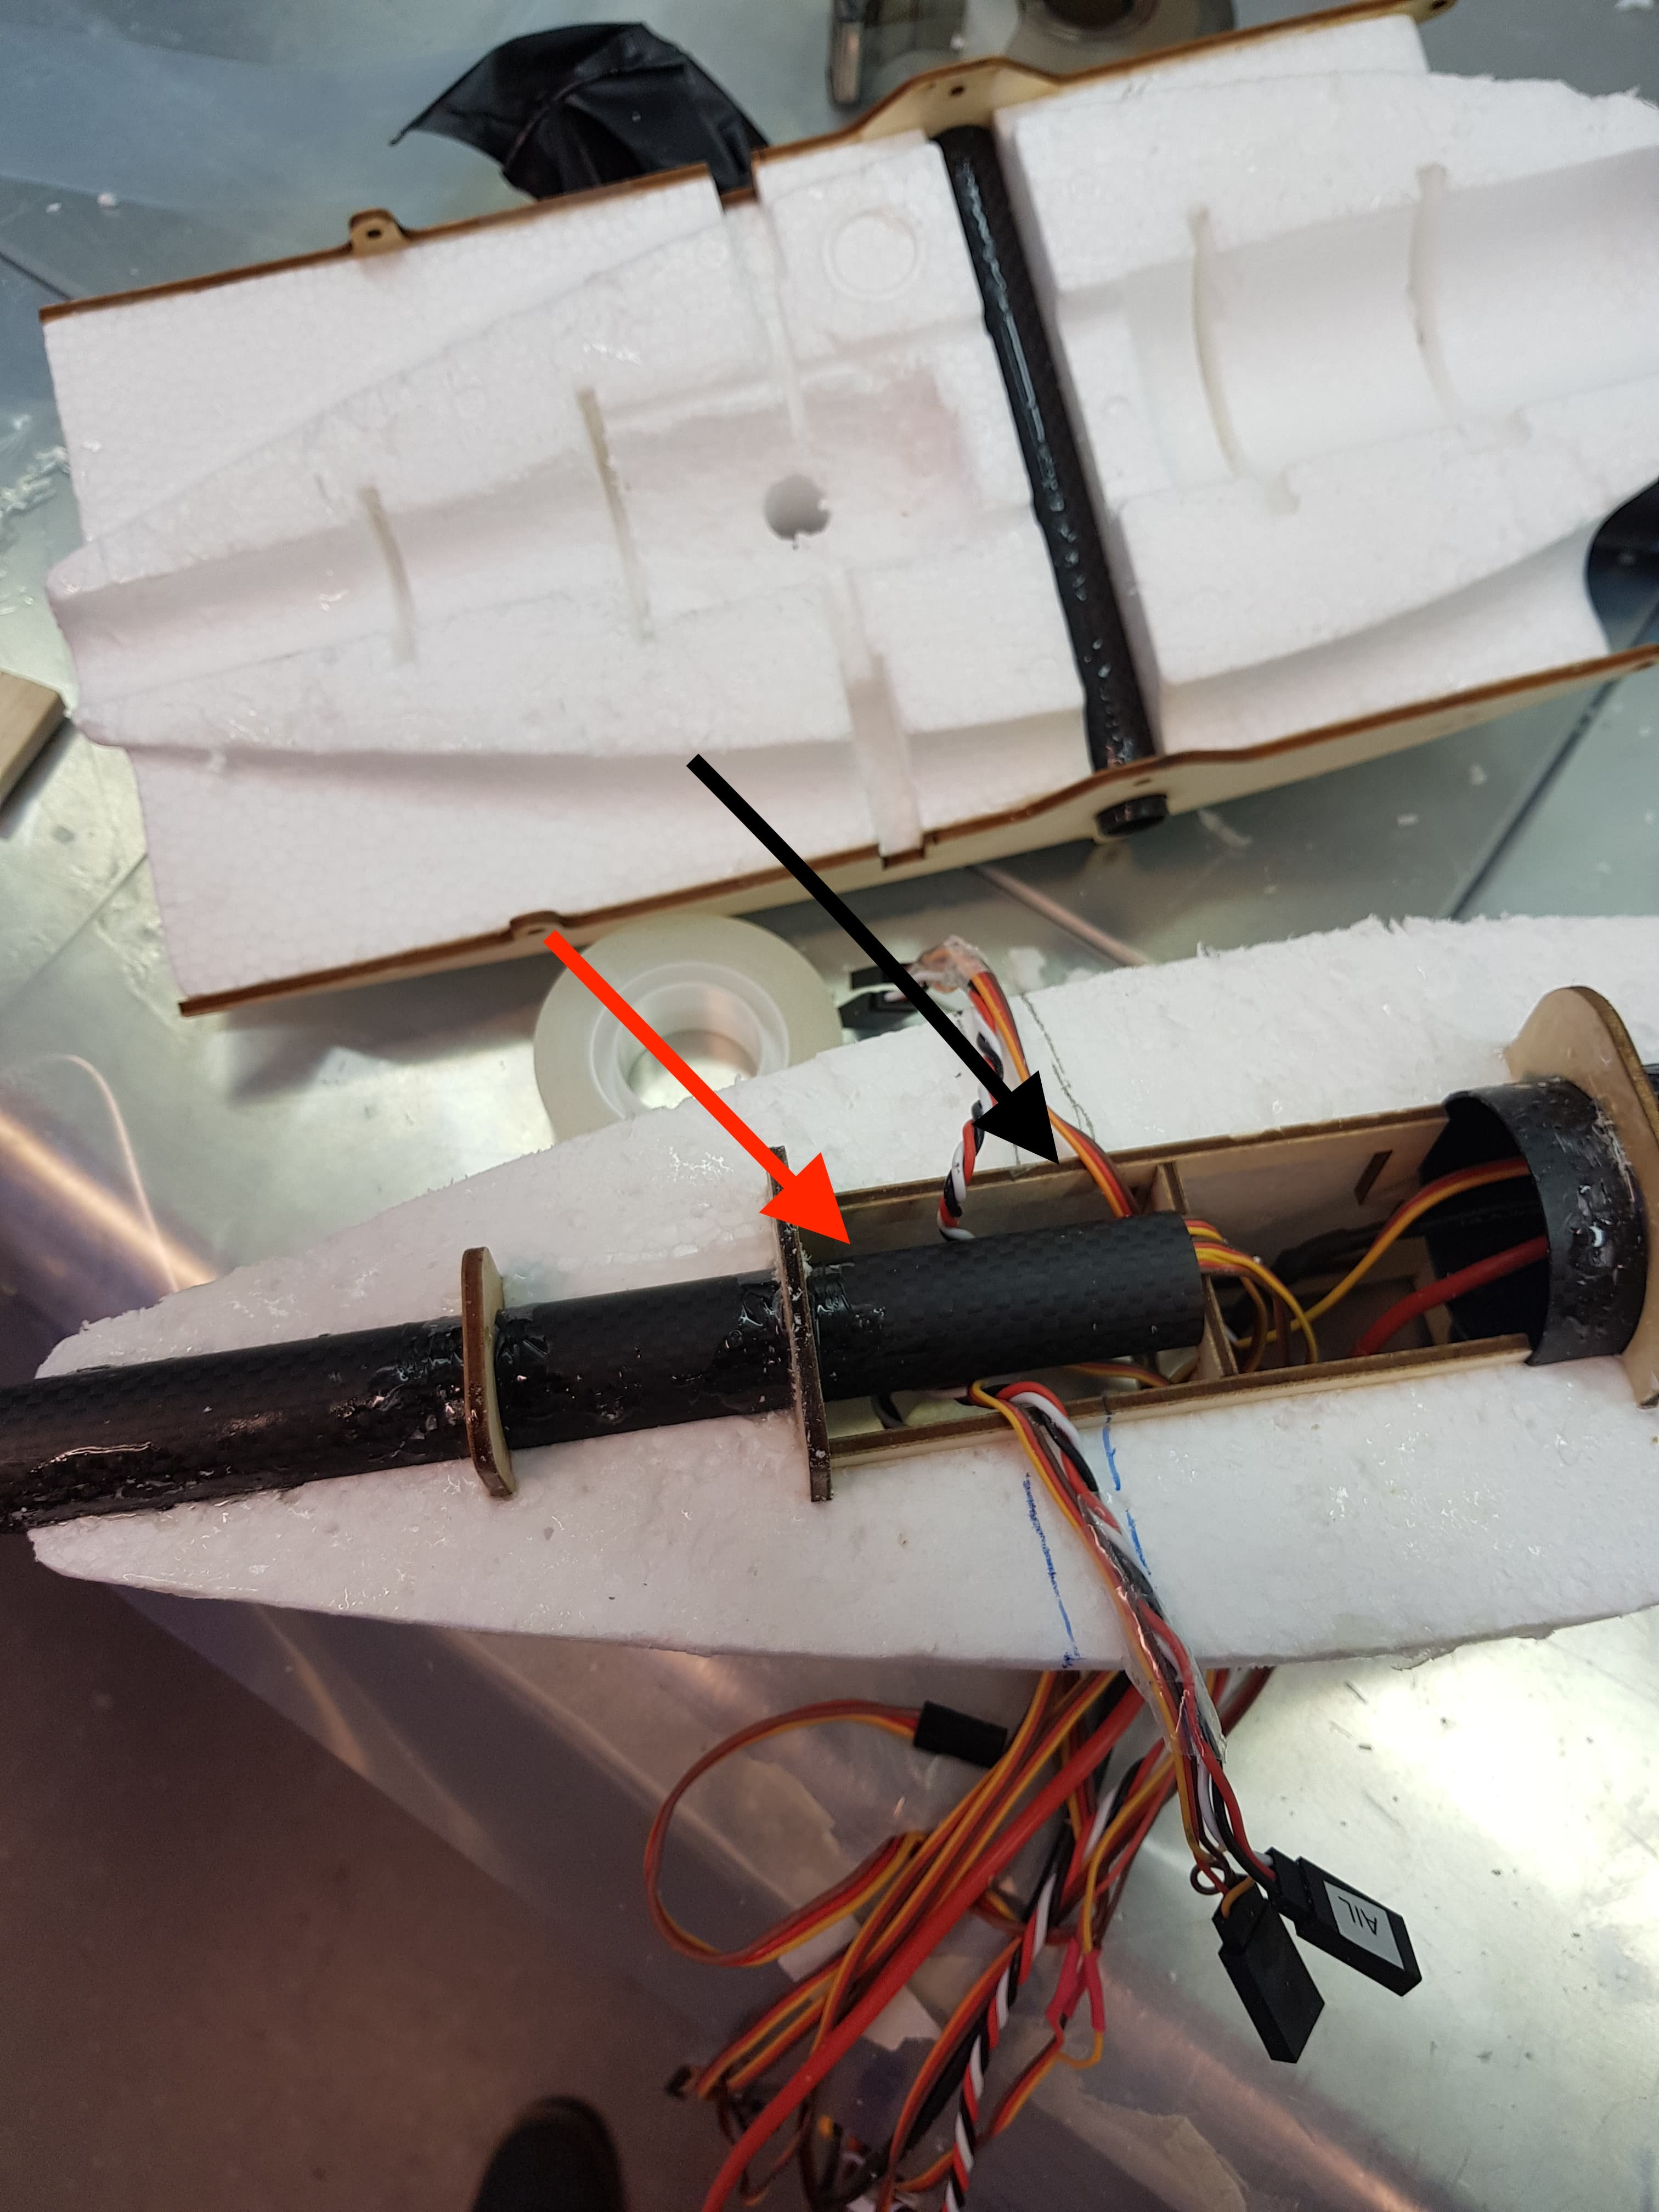
\includegraphics[height = 7cm, width = .6\textwidth]{bilder/feilmontering_av_karbon_red.jpg}
	\caption[Feilliming]{Det bakre karbonrøret ble limt for langt frem, og blokkerte for eventuell GPS-installasjon og påmontering av øvre ramme. Karbonrøret skal egentlig være ved den røde pilen.}
\end{figure}

\begin{figure}[ht]
 \centering
 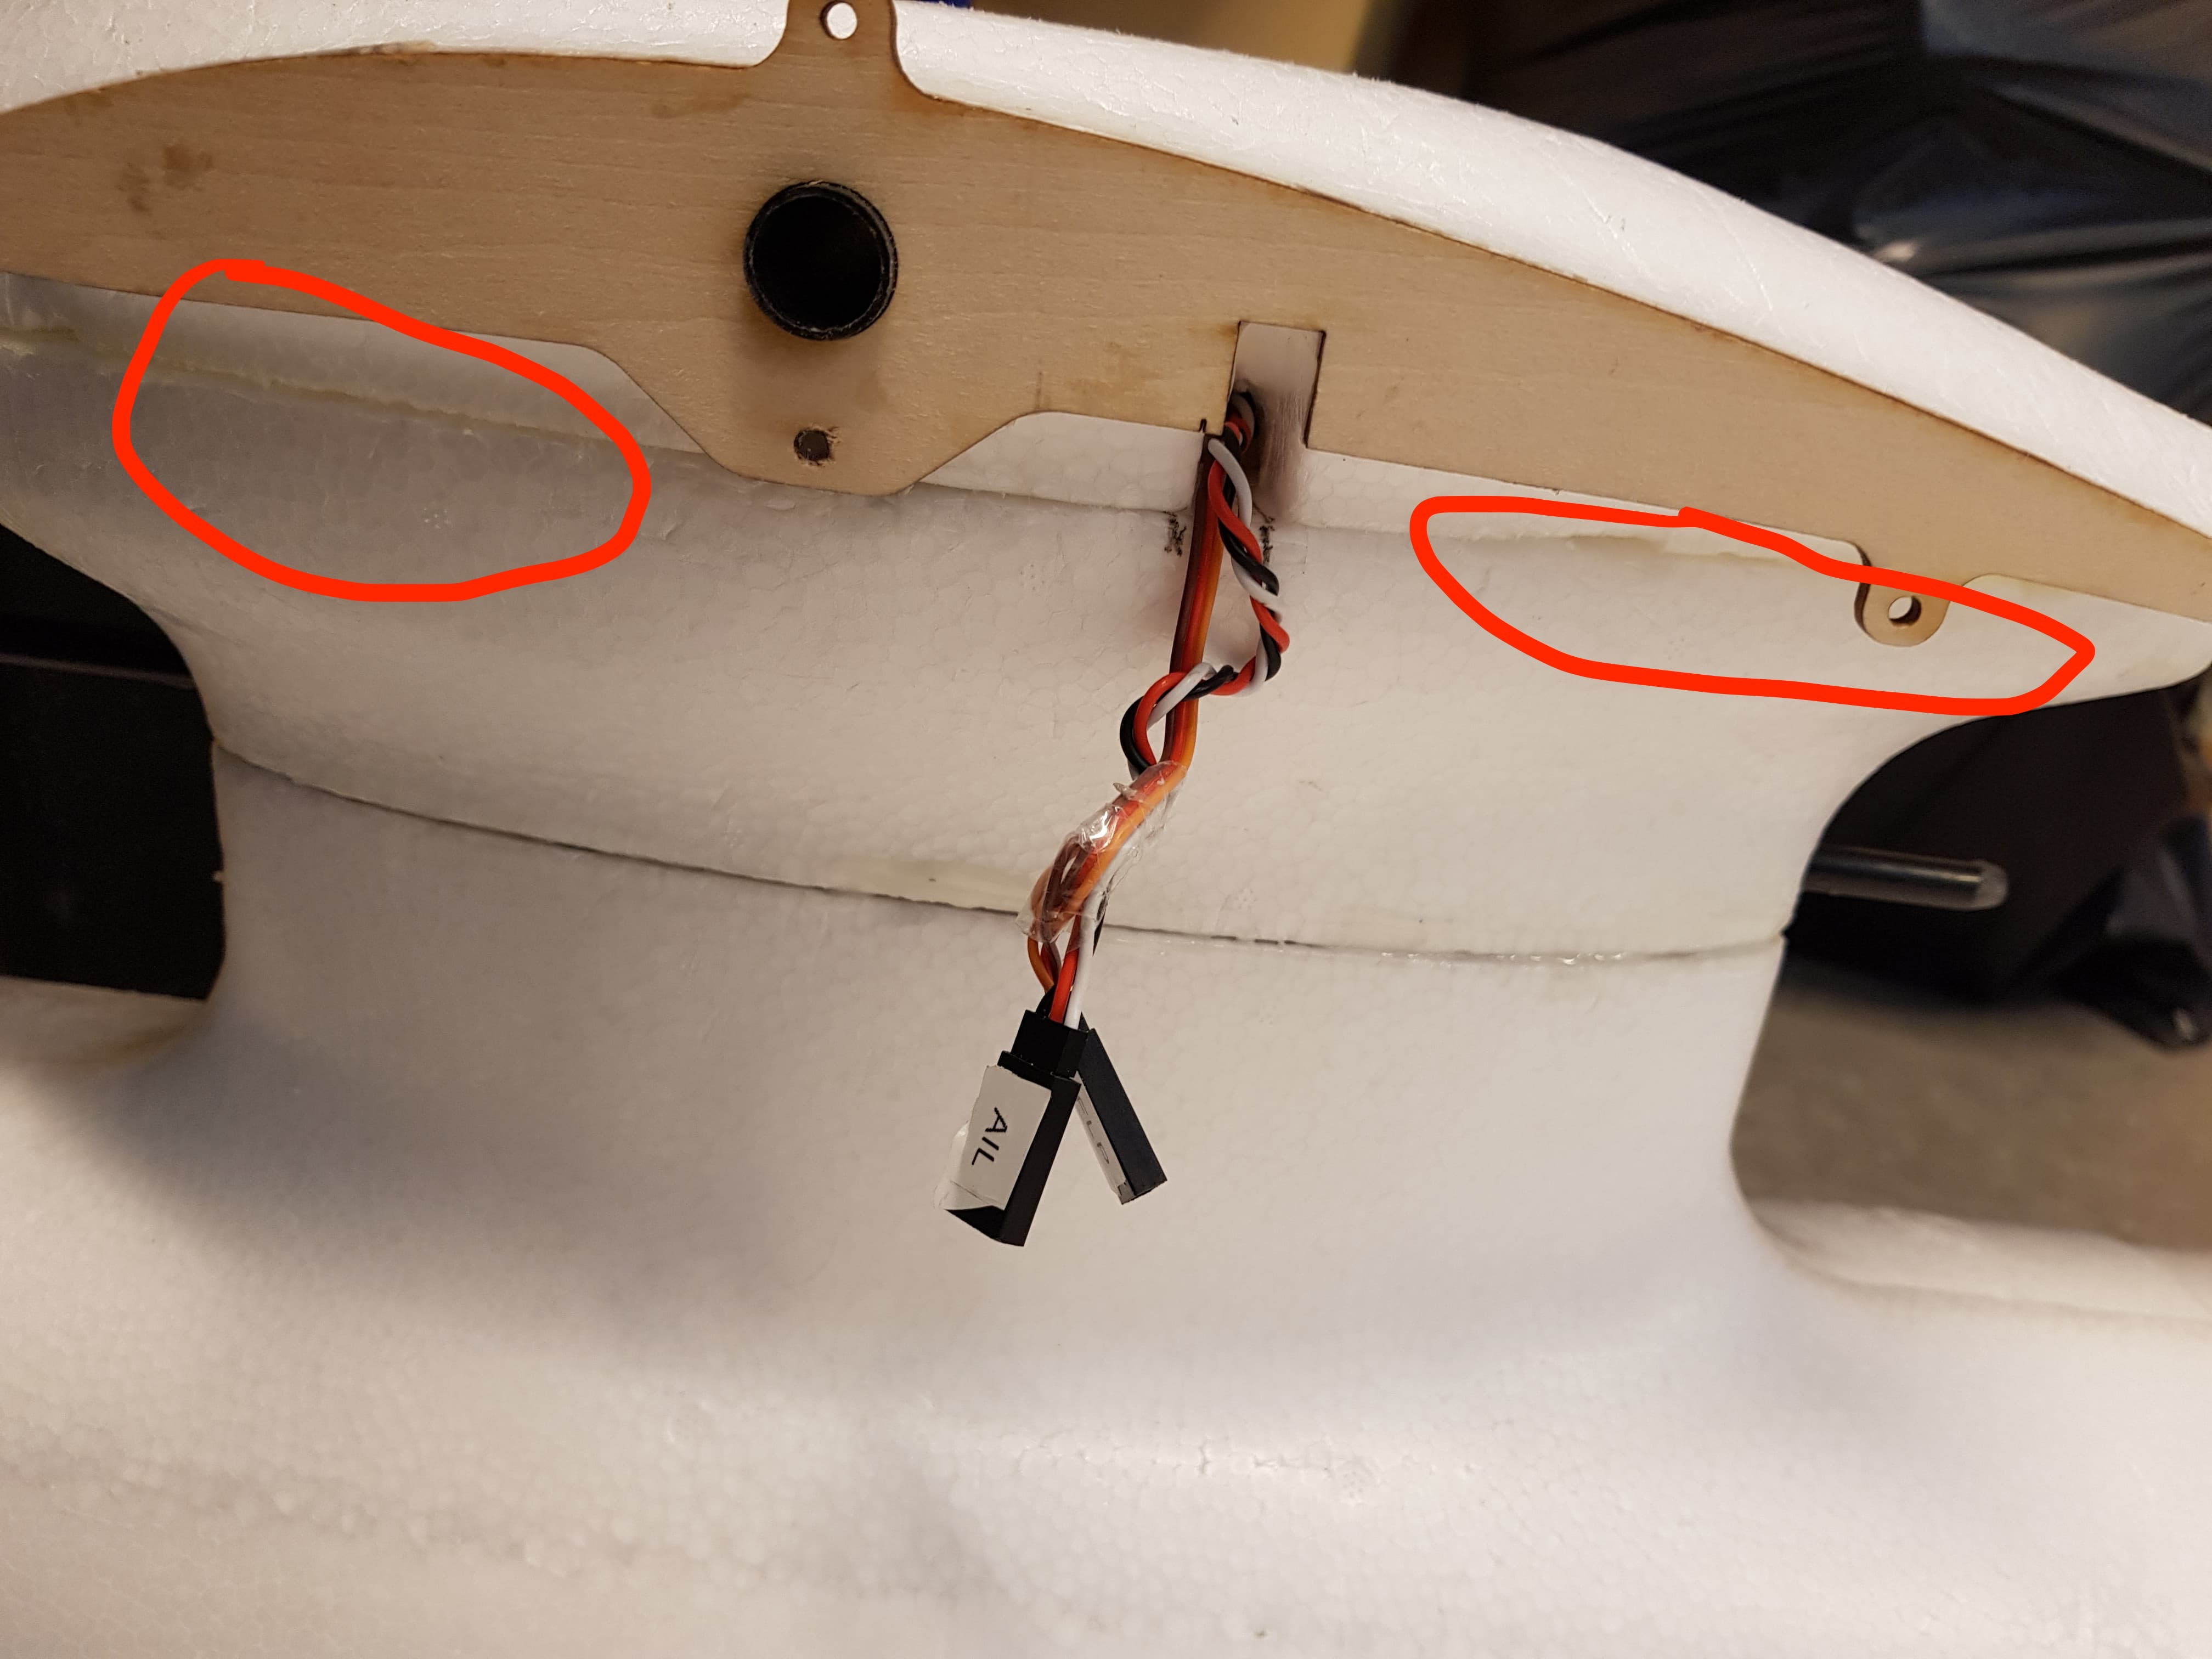
\includegraphics[height=7cm, width = .6\textwidth]{bilder/fylling2_red.jpg}
 \caption[Endelig limeresultat]{Endeling resultat av limingen. Merk det fylte området.}
\end{figure}
\newpage

Mens dette sto og herdet, fortsatte jeg arbeidet ved å montere halen. Jeg glemte å ta bilder av denne monteringen. Etter halen gjenstod monteringen av utstyrskammeret. Dette kammeret festes med flykroppen ved hjelp av et karbonrør gjennom begge delene, men Norut foretrekker at de er limt sammen med epoxy i tillegg til karbonrørets funksjon. Deretter ble det bare å montere på vingene, koble halen fast, og flyet var klart for første inspeksjon

\begin{figure}[ht]
	\centering
	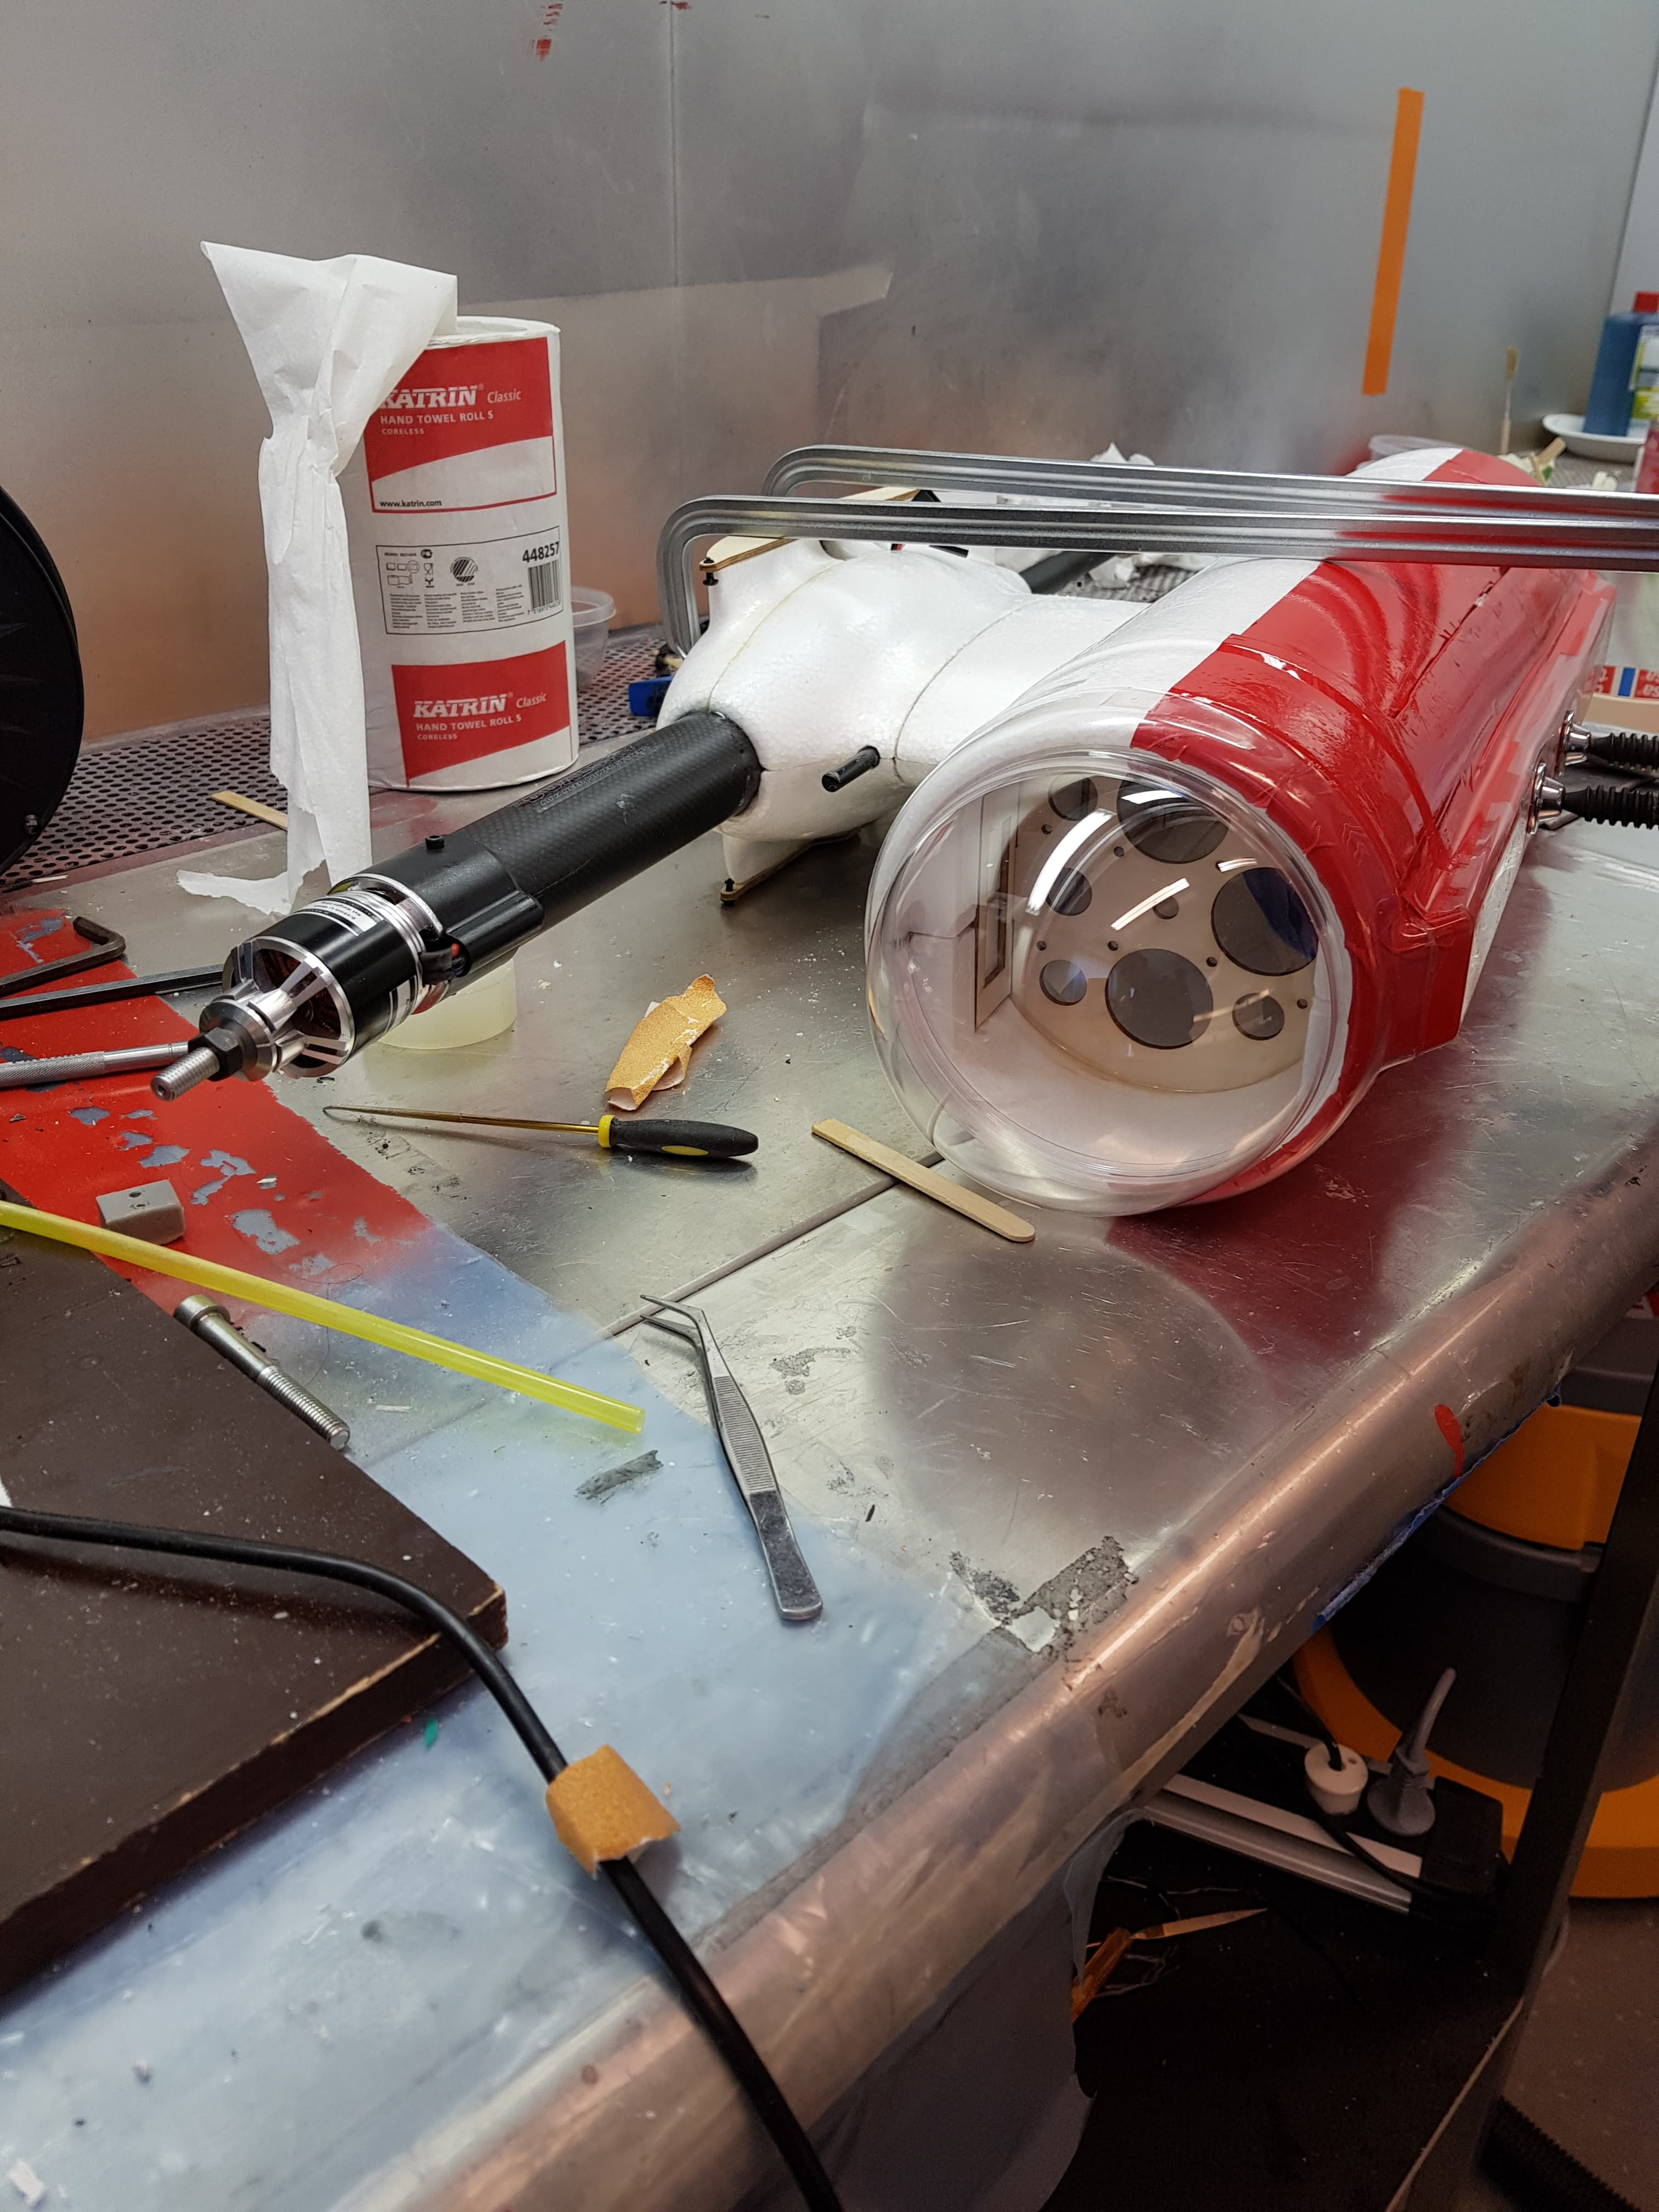
\includegraphics[width = .5\textwidth, height = 8.1cm]{bilder/kammermontering.jpg}

	\caption[Herding av epoxy]{For å holde delene sammen under herding, brukes klemmer for å presse hardt ned. Her ble det brukt 30-minutters epoxy. Det er likevel lurt å la den ligge ''ut dagen'' for best mulig feste.}


\end{figure}
\newpage
\subsubsection{Inspeksjon}
For at et luftfartøy hos Norut skal kunne flys, må det godkjennes og erklæres luftdyktig av teknisk personell. Det første flyet ble ikke godkjent, da halens horisontale stabilisator ikke var i vater. Etter en rask borring av nytt hull i karbonbommen som holder halen fast til selve flykroppen, ble flyet godkjent. Nå kunne elektronikken legges inn. \\

\begin{figure}[ht]
	\centering

	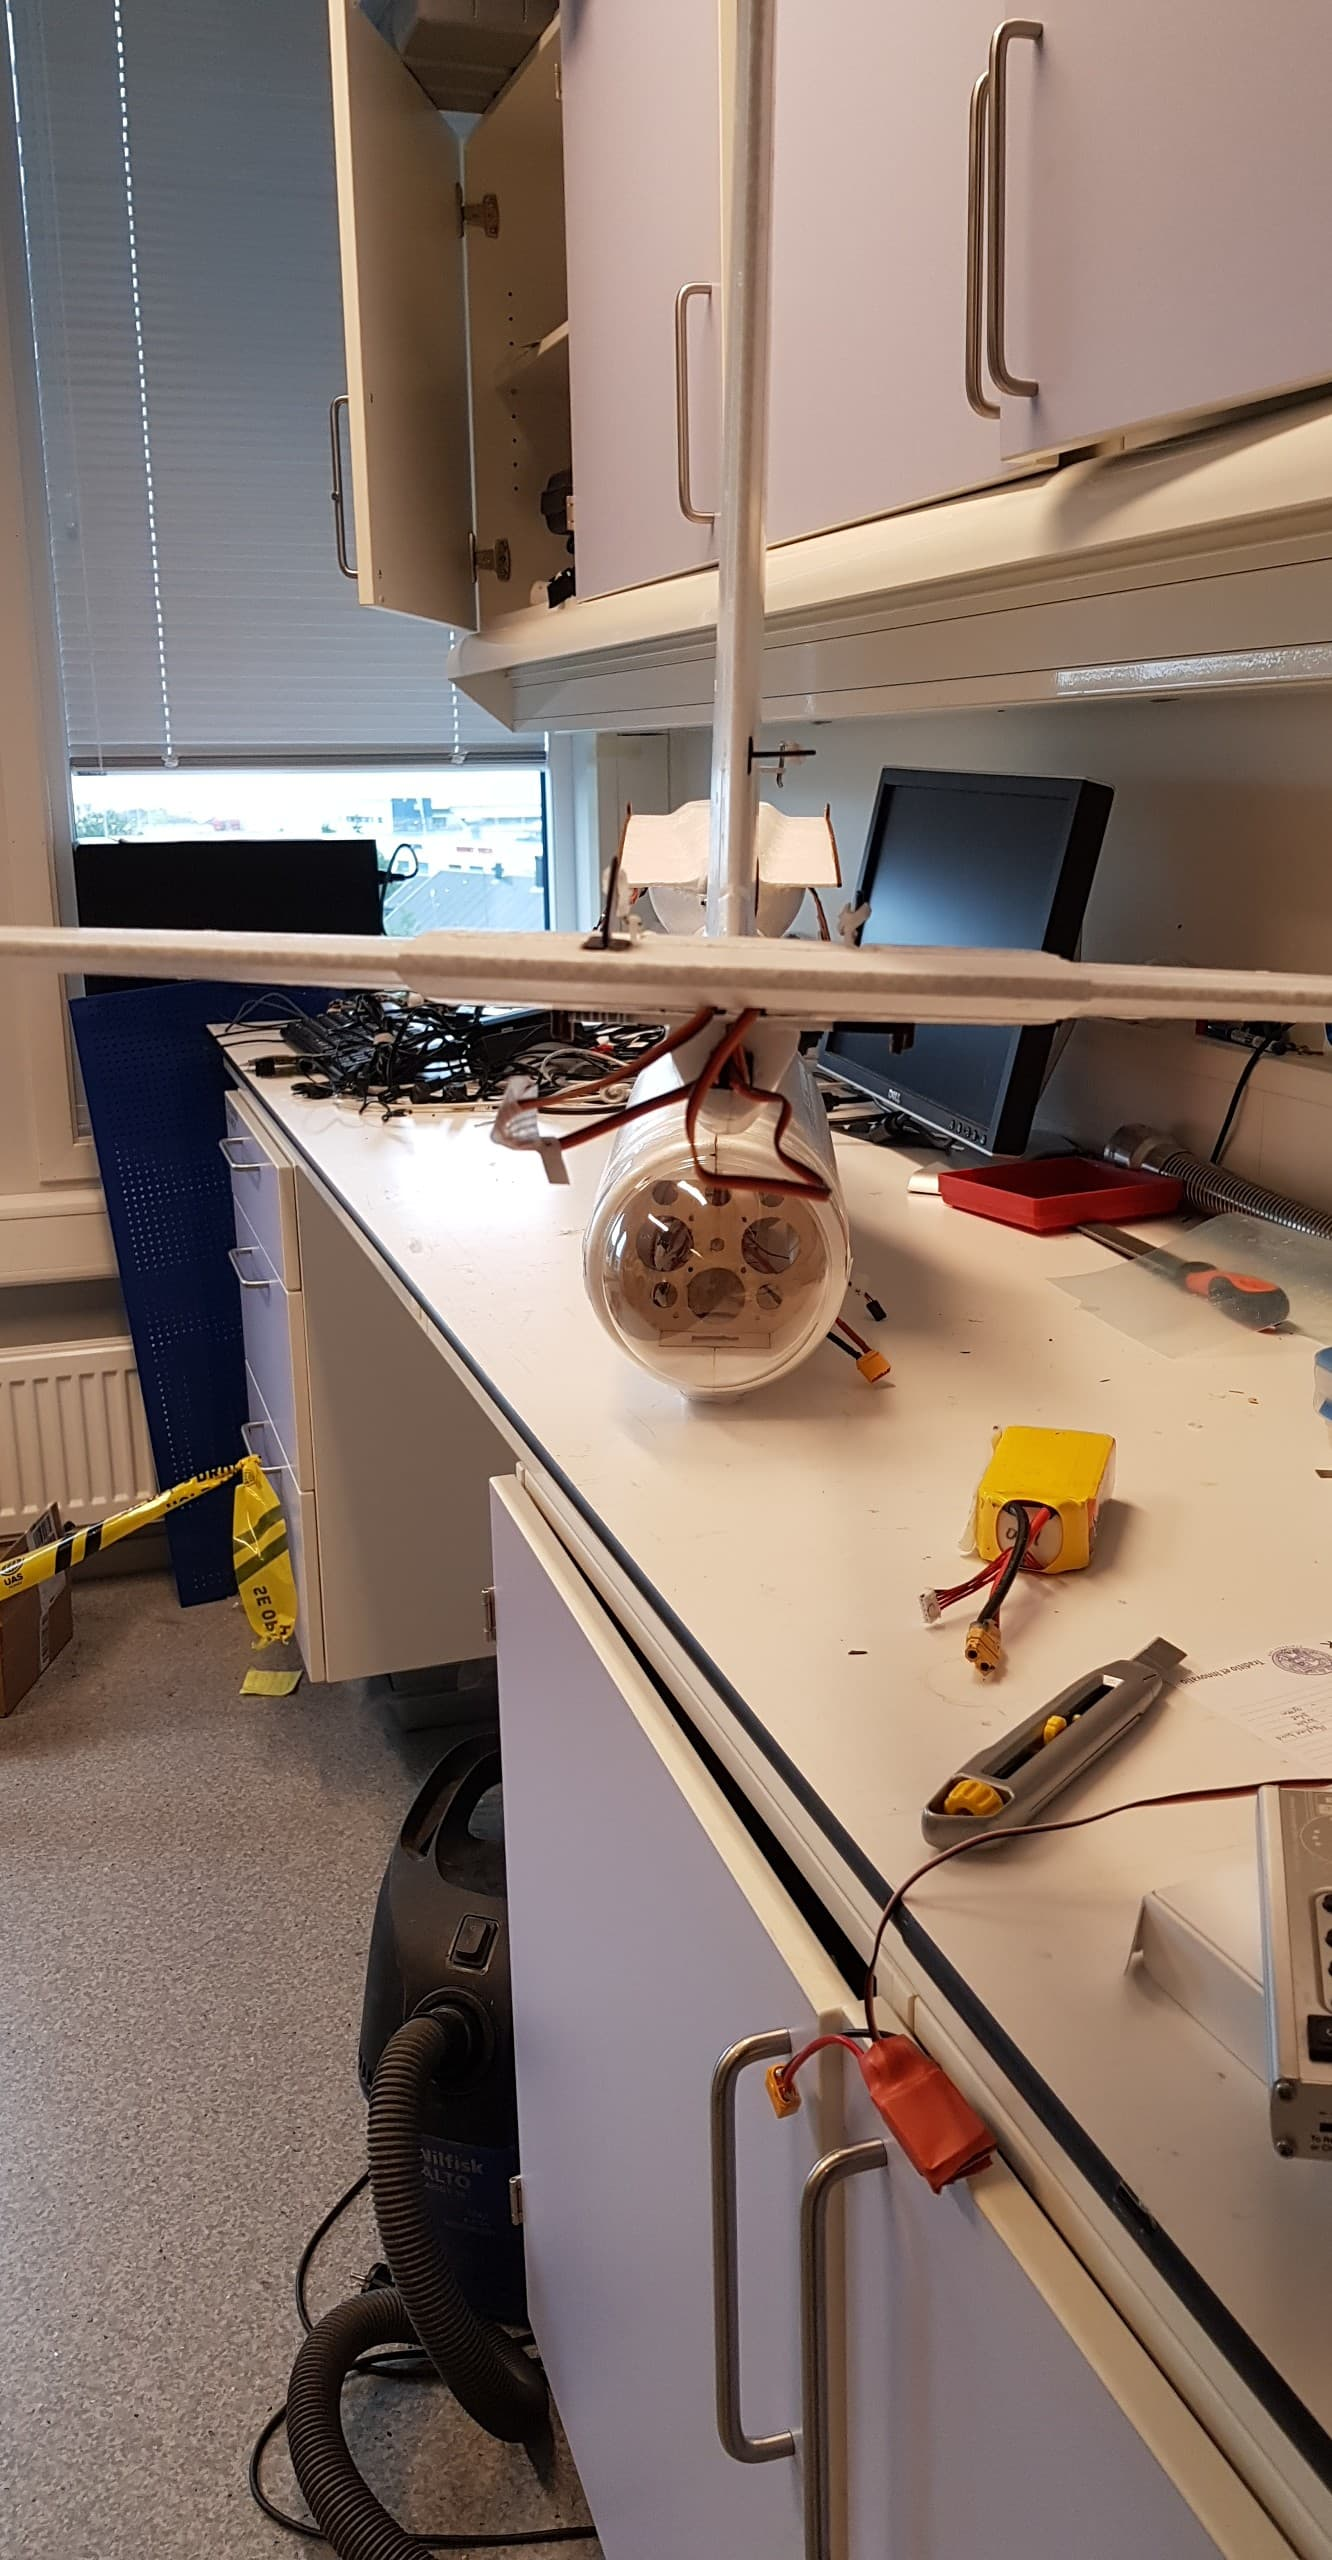
\includegraphics[width = .5\textwidth, height = 10cm]{bilder/skjev_halefinne.jpg}
	\caption[Skjev stabilisator]{Den vertikale stabilisatoren er ikke normal på den horisontale stabilisatoren, og gjør flyging ikke optimalt. Den kan funke, men sideroret må trimmes betraktelig for dette. Det begrenser det totale utslaget.}
	
\end{figure}

Da det første flyet skulle være en trainer, har den bare det mest nødvendige, altså en RC-link. Alt som måtte da gjøres var å montere mottakeren inni kammeret og koble servokablene til denne. Deretter kalibrere og mappe servo-utgangene, og flyet var klart.

\begin{figure}[ht]
	\centering
	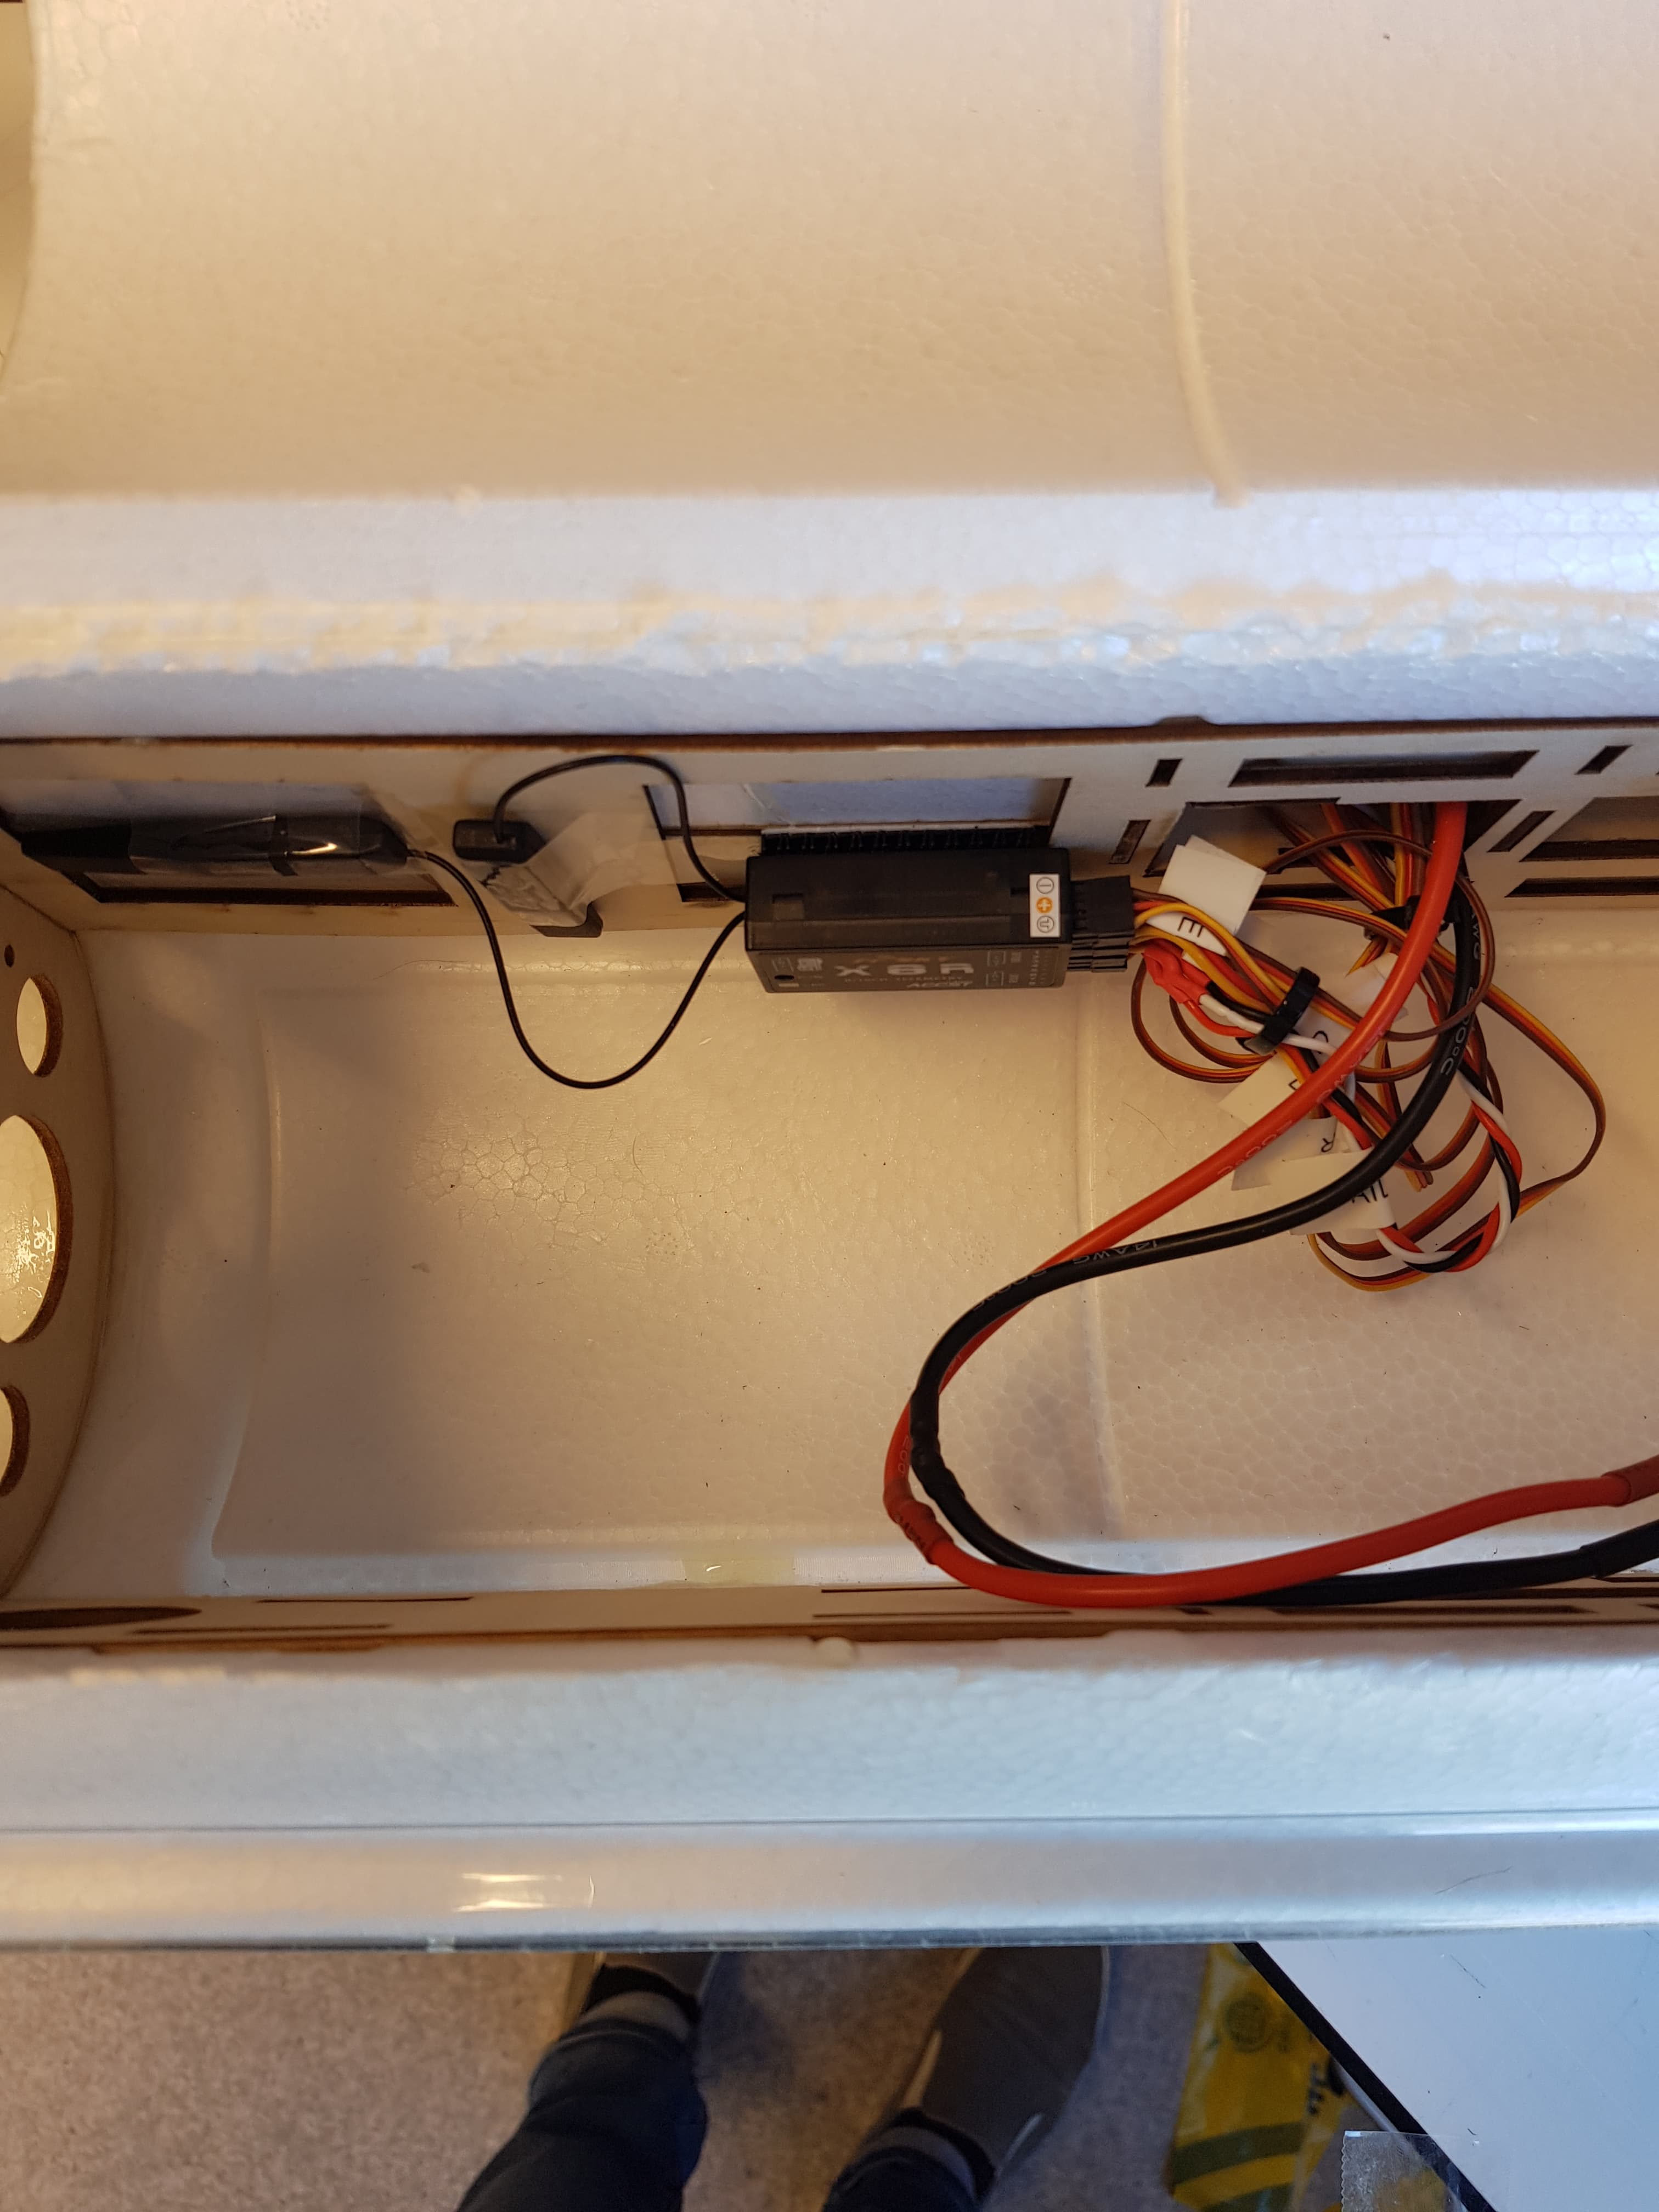
\includegraphics[height=8cm, width = .6\textwidth]{bilder/mottakermontering.jpg}
	\caption[Mottaker-montering]{Ferdig montering av X8R-mottakeren inni Observer-trainer'en. PCB-antennene er plassert i en \ang{90}-orientering for best mulig signalspekter. RC-linken her er PWM-regulert, og benytter én kanal for hver utgang.}
\end{figure}
\newpage

Ved dette oppsettet av RC-linken brukes det totalt 8 kanaler, som er maks antall på denne mottakeren i PWM-konfigurasjon. Alternativt kunne man ha holdt seg til 6 kanaler, der flap-klaffene og balanserorene kobles i parallell. Det uheldige er at da må hver enkelte roroverflate være helt sentrert, slik at bevegelsene er synkron. I tillegg blir det mer jobb med å få servoene til å ``gå riktig vei''. Å holde kanalene uavhengige av hverandre gjør dermed arbeidet mye enklere og oversiktligere. 

\begin{figure}[ht]
	\centering
	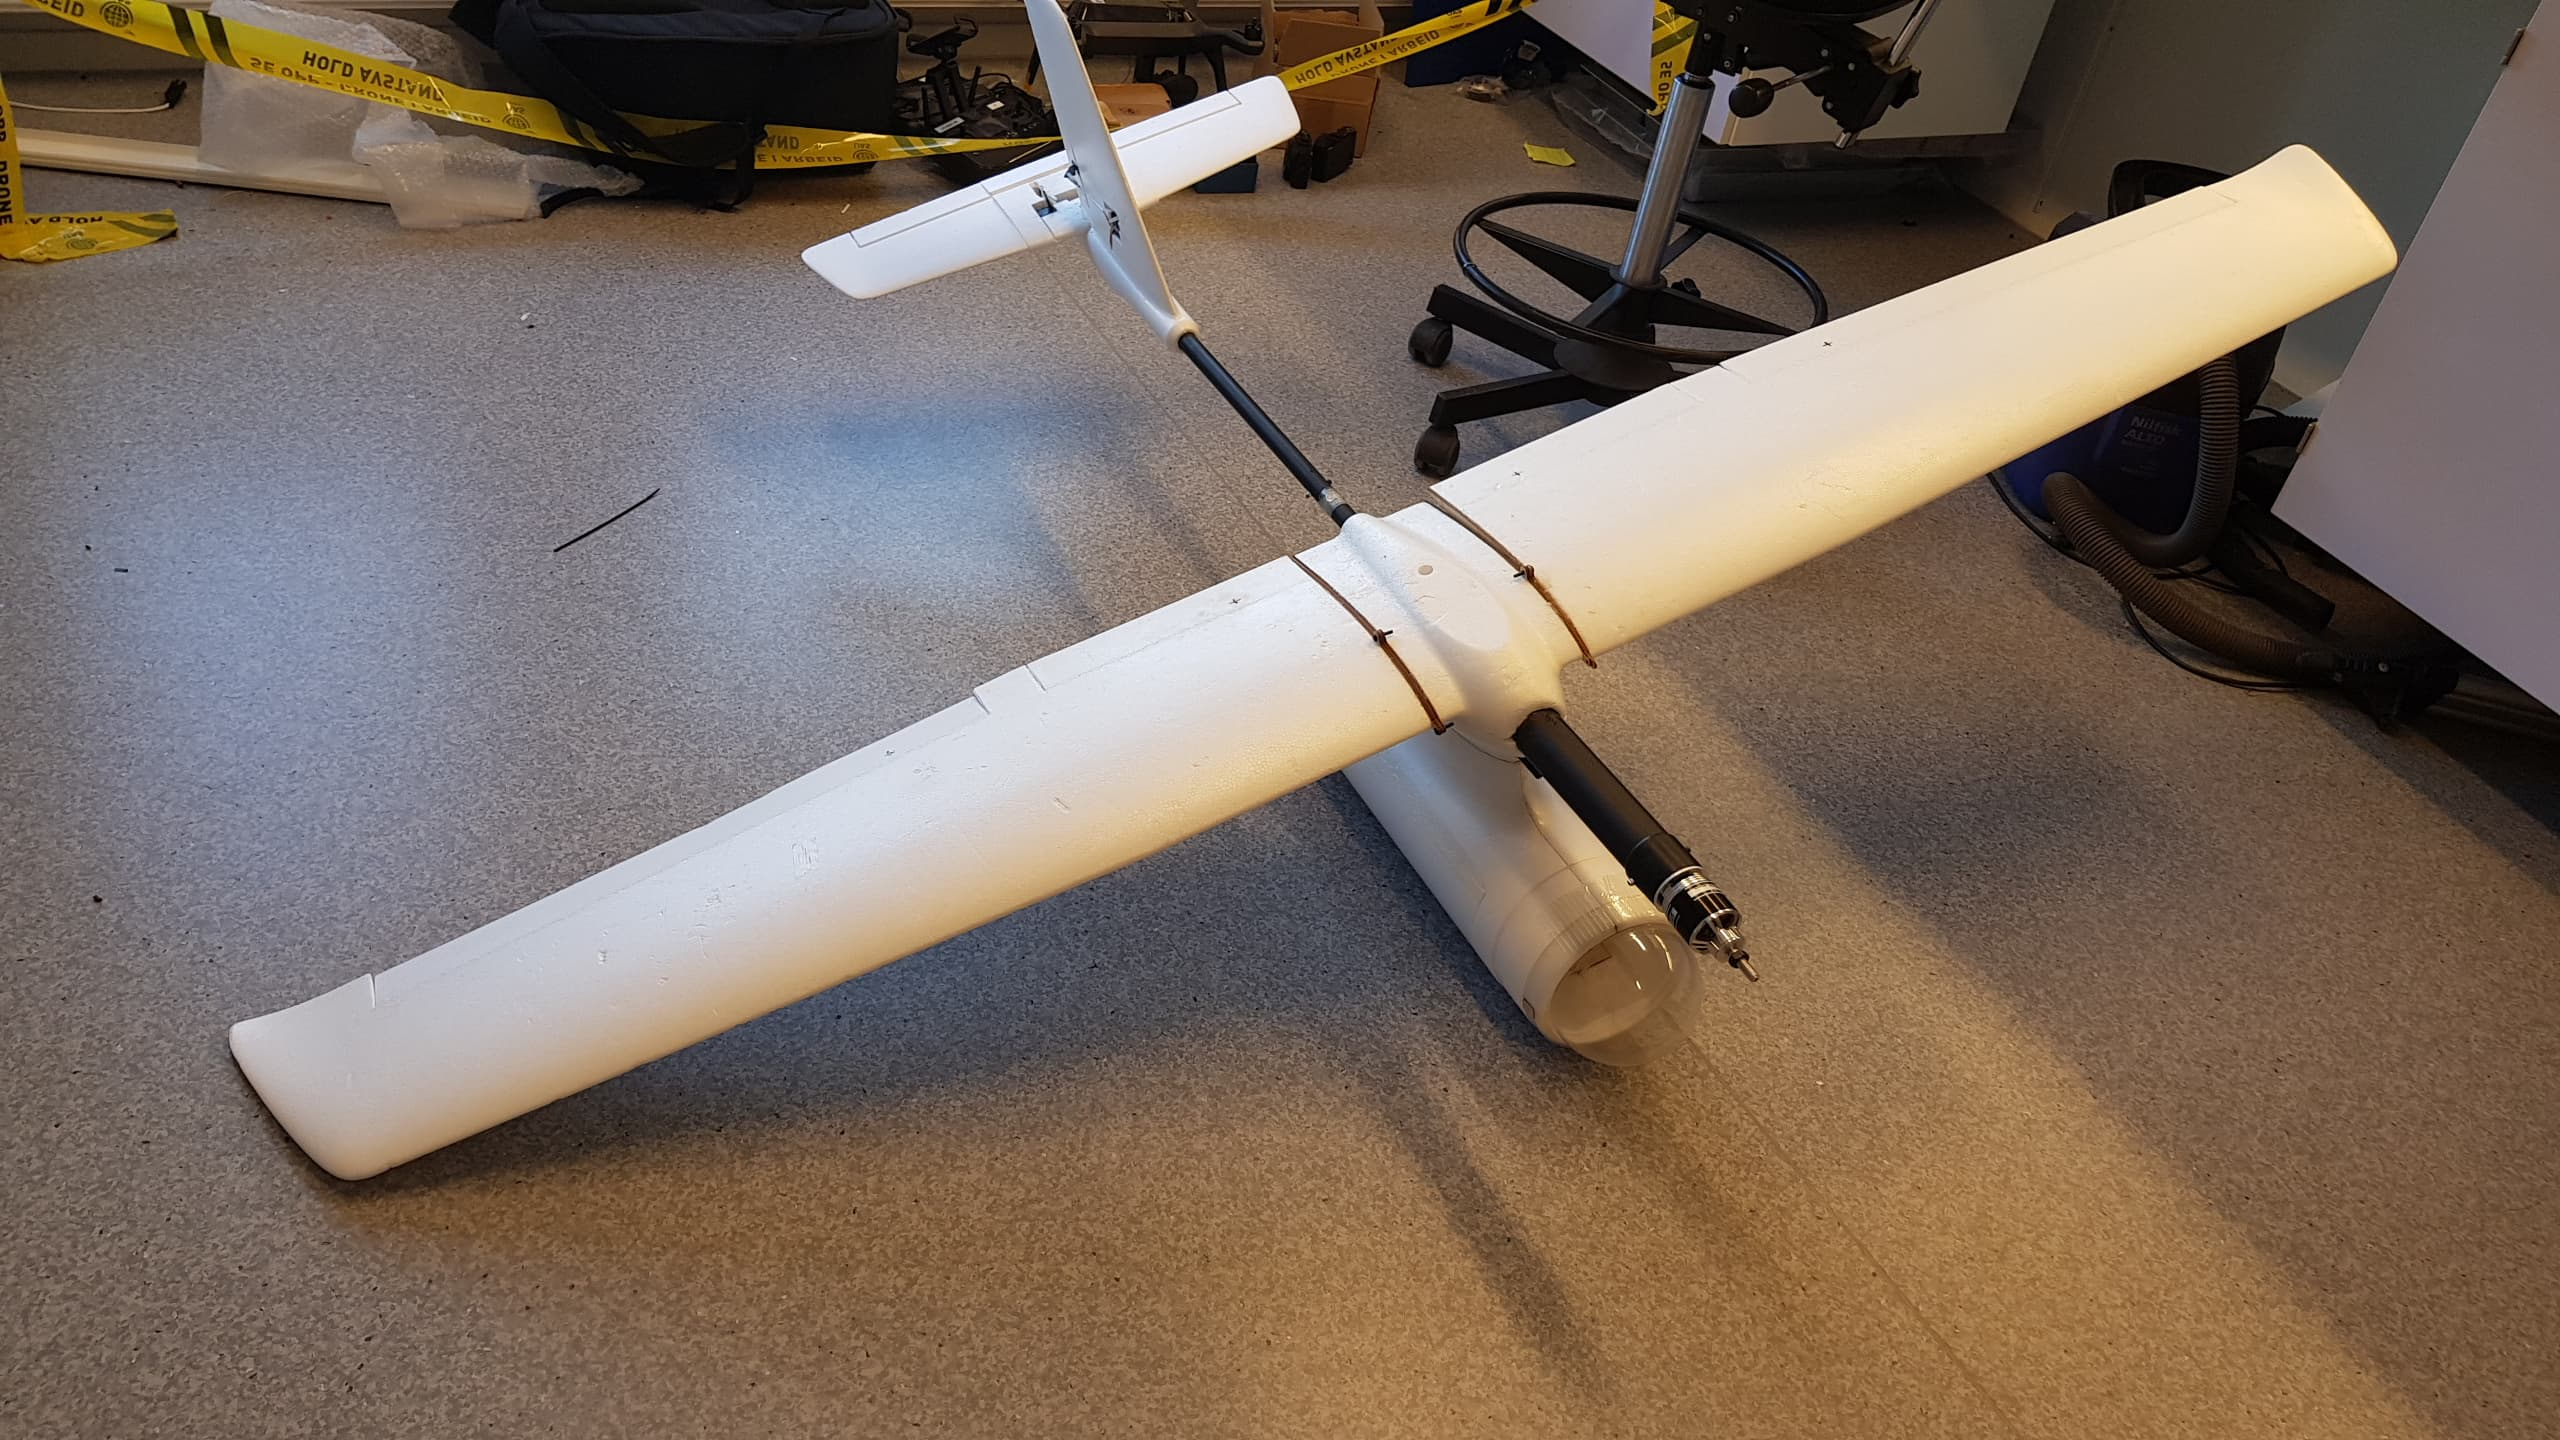
\includegraphics[width=.6\textwidth, height = 6.5cm]{bilder/forste_fly_ferdigstilt.jpg}
	\caption[Trainer-fly]{Trainer - flyet ferdig konfigurert, med vingespenn på 2m, og lengde på 1.5m. Byggingen av denne tok omtrent 1.5 uke. }
\end{figure}

Da jeg hadde fått erfaring av byggingen av den første modellen, gikk det hurtigere å bygge den andre. Med kombinasjon av ``fersk minne'' og noen deler som allerede var ferdiggjort i Bodø, ble nr.2 ferdig på 2 dager. For denne modellen gjenstod å montere og kalibrere servoer på overflatene, kalibrere fartsregulatoren og feste kroppen sammen. Oppsettet av avionikken fikk jeg ikke gjennomføre, da Norut selv vil gjøre denne delen. Det ble ikke anledning for meg å kunne observere installasjon, da dette skulle tydeligvis gjøres etter endt praksisperiode. \\
Modellen skulle installeres med utstyr for såkalt mapping-formål. Luftfartøyet følger et gridmønster satt opp ved hjelp av en bakkestasjon. Luftfartøyet har forbindelse med bakkestasjonen ved hjelp av en data-link, slik at flyet kan styres utenfor radioens 2.4GHz - rekkevidde. For dette formålet benyttes en Pixhawk - autopilotsystem. I tillegg monteres på ulike sensorer for sikker og koordinert flyging. Dette inkluderer pitot-rør (for hastighetsmåling), spenningssensor, strømsensor og høydemåler. 

\begin{figure}[h]
	\centering
	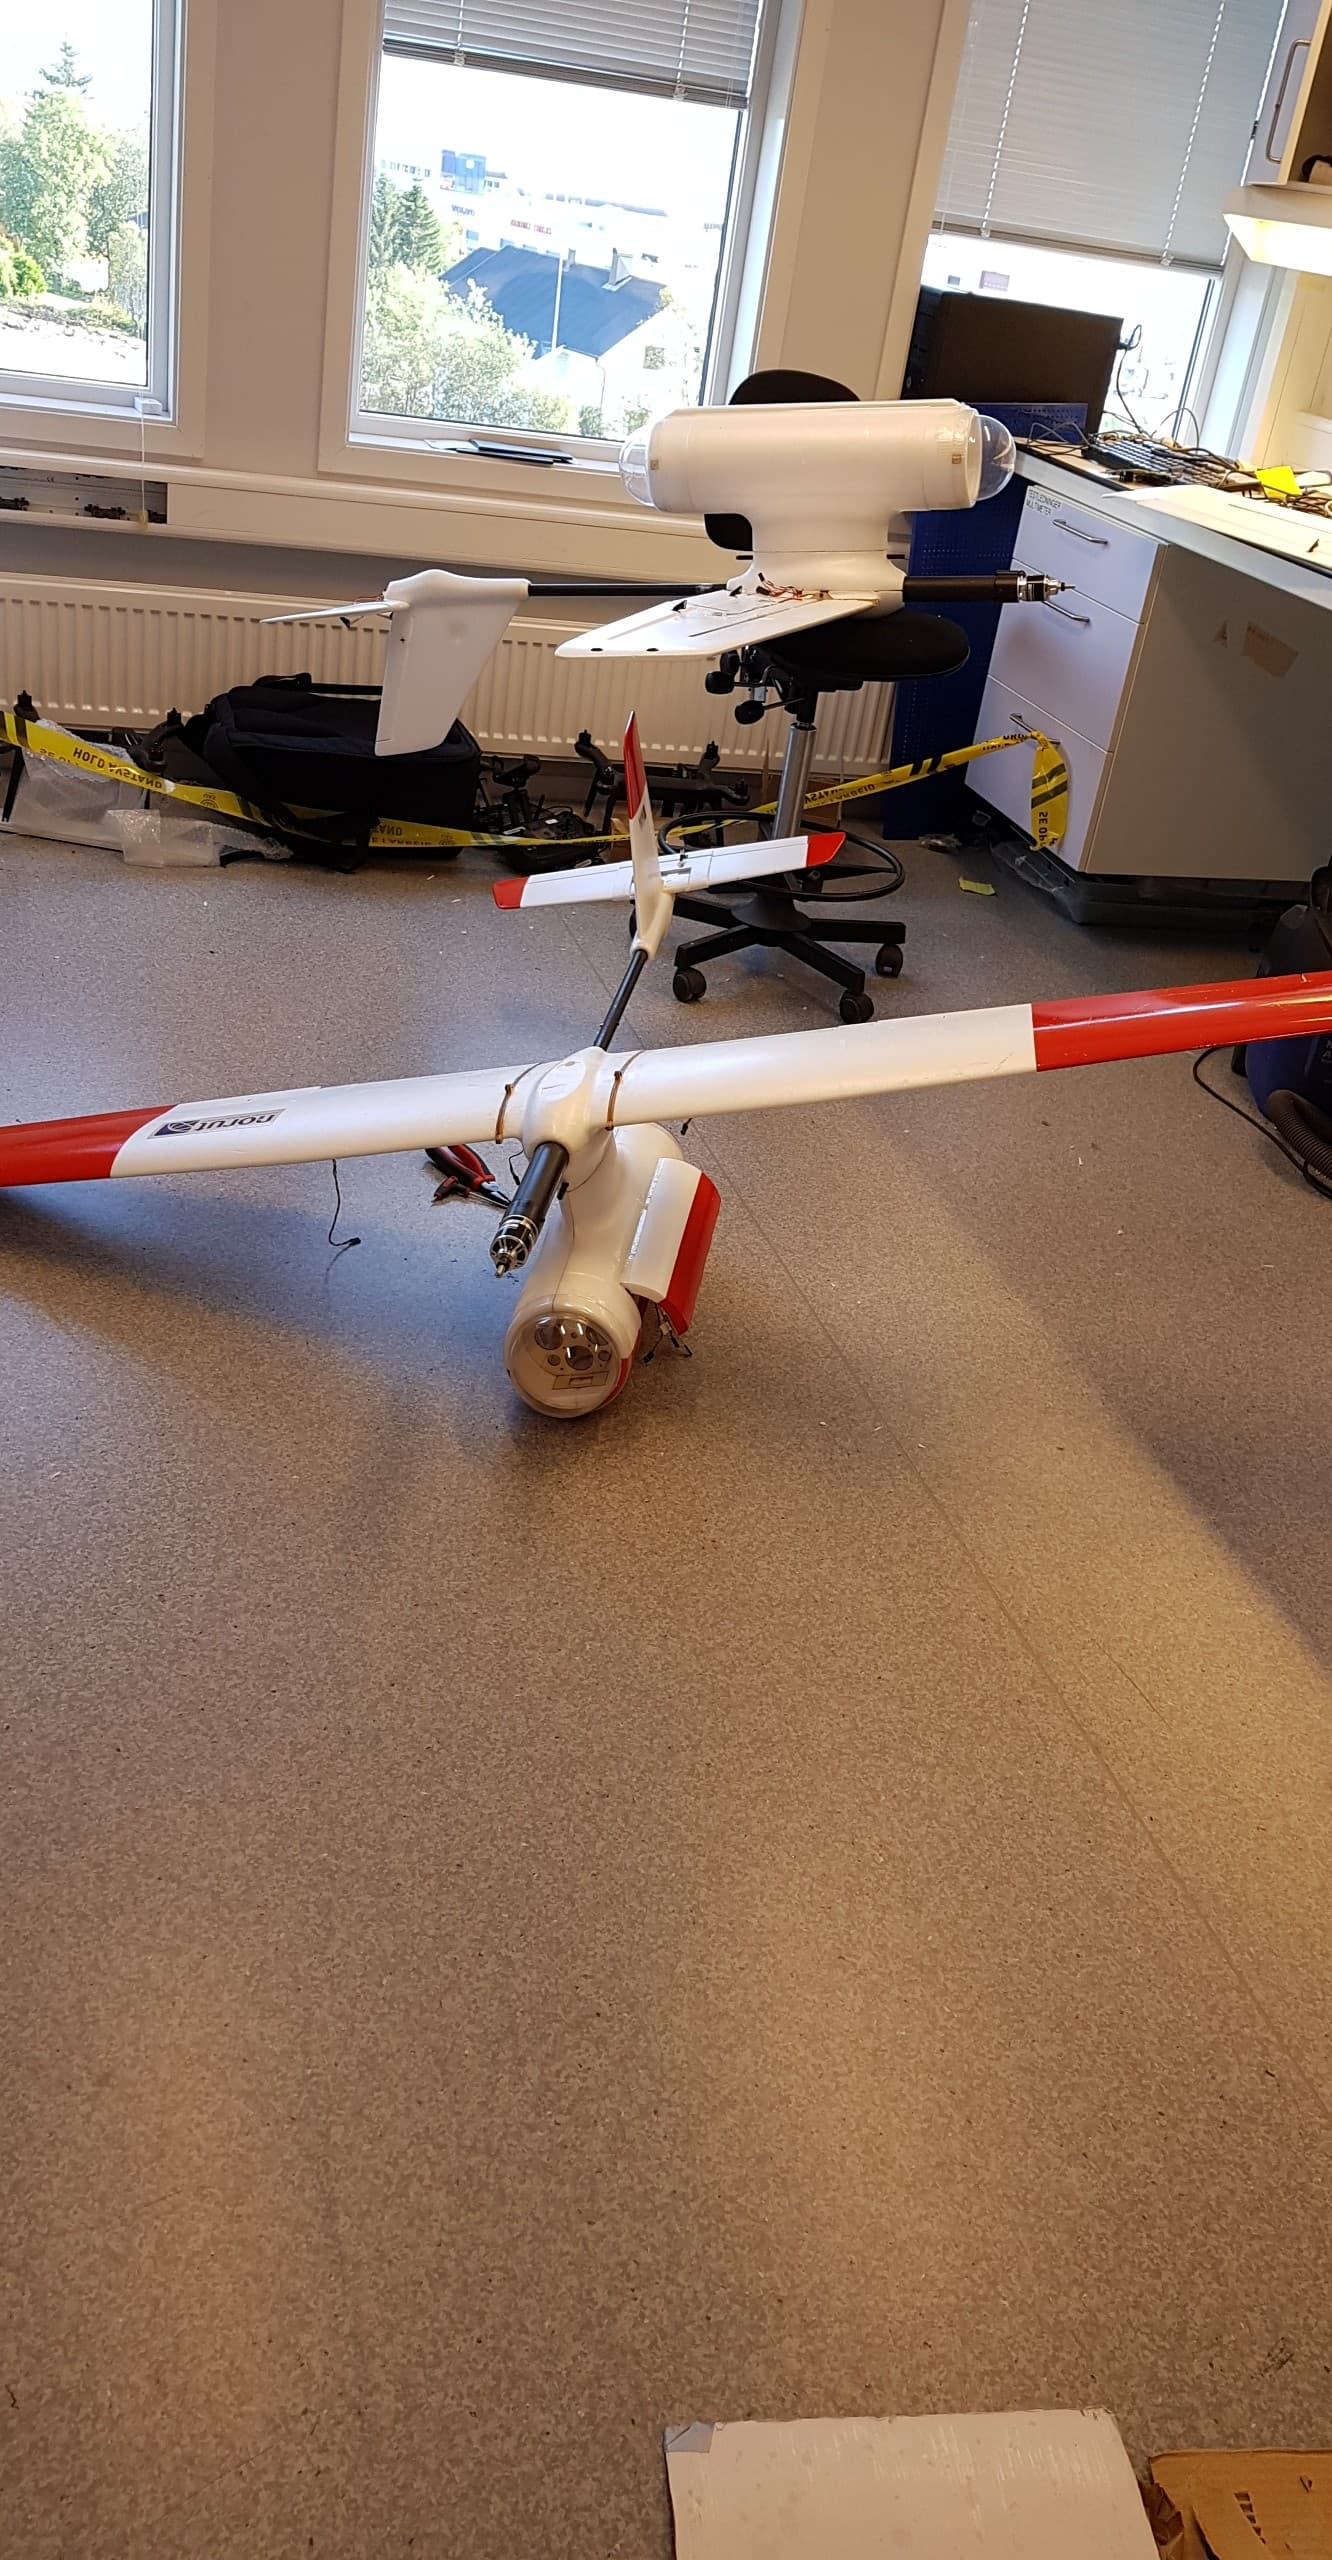
\includegraphics[width = .4\textwidth, height = 9cm]{bilder/andre_fly_ferdigstilt.jpg}
	\caption[Fly nummer to ferdig]{Fly nr. 2 ferdig. Dette skulle monteres med mer avansert utstyr enn traineren i bakgrunnen.}
\end{figure}

\subsubsection{Testflyging}
På den siste arbeidsdagen ble det mulighet for å gjøre testflygning. I forkant av dette ble flyet forberedt til flyging. Servoer sjekkes, eventuelle skader fikses, og flyet monteres. I tillegg må et skjema sendes inn og godkjennes av operativ leder hos Norut. Et slikt skjema kalles for Mission Acceptance Form (MAF). Det inneholder opplysninger om den type flyging som skal gjøres, flytype, personell til flyging, risikoanalyser med mer. Vedlegg 4 viser UiT's Mission Acceptance Form. Hver operasjon som gjennomføres hos Norut må ha godkjent MAF av operativ leder. \\

Da vi ankom Finnvikdalen for testflygingen gjennomgikk vi monteringen av flyet og  briefet hverandre om take-off og videre flyging. Deretter gjennomførte vi en run-up, der vi tester motorens ytelse samt servoenes utslag. Vi oppdaget på run-up at motoren slet etter 70\%. Vi mistenkte at det hadde noe å gjøre med en usynkronisert fartskontroller eller eventuelle koblingsfeil. Vi ignorerte disse ``varslene'' og bestemte oss for å fortsette. \\
\newpage
Ved take-off skjedde det jeg hadde en mistanke om: Motoren begynte å hakke, og i panikk tok jeg throttelen helt ned, noe som gjorde at flyet steilet på venstre vinge og gikk i bakken. Vi skulle ha tatt hintet og ikke tatt av i det hele, men det er vel slike feil man lærer av. Halen på flyet løsnet og det ene pleksiglasset på kammeret ble knust. 
Hvis ulykken hadde vært mer alvorlig, f.eks personskade, skulle dette rapporteres til Luftfartstilsynet. Det skulle opprettes en ticket og flyet blir holdt på bakken til dette blir fikset. En ticket er en notis som beskriver feil på luftfartøyet og årsaken til feilen. Det er nødvendig å føre tickets for å kunne dokumentere flyets luftdyktighet.\\

``Uheldigvis'' var jeg ferdig på praksisperioden min etter denne dagen og fikk dermed ikke muligheten til å fikse disse skadene. Reparasjonsarbeidet måtte etterlates til de andre ingeniørene på avdelingen.\\ Dermed fikk jeg heller ikke muligheten til å føre inn flyets egenskaper i dens POH, noe som var leit, men avdelingssjefen var likevel fornøyd med arbeidet som hadde blitt gjort; testflyvninger går ikke hele tiden på skinner. \\
Et viktig poeng ble også satt fra dette: Dersom det er tvil på det tekniske når en er ute på flyvning, avlys heller flyvningen enn å risikere å ødelegge luftfartøyet. Dette er nok et typisk eksempel på ``learning by doing'' - prinsippet. I situasjoner der konsekvensene forekommer av feil beslutning, kan det tas til lærdom for neste gang, og gjøre testflygningsprosedyrene sikrere. \\

Jeg er likevel litt overrasket over at Norut tillot meg å gjennomføre testflyvningen til tross for at vi oppdaget feilen ved run-up og at jeg var fartøyssjefen for testflygningen. Det var muligens litt pedagogisk i samme sleng, da jeg fikk litt trening i hvordan det er å være ansvarlig for operasjonen.  


\newpage
\section{Refleksjon over praksisperioden}
\subsection{Arbeidsforhold}
En ting som jeg oppfattet i løpet av første uke hos Norut var det svært travle arbeidsmiljøet. Norut skulle gjennomføre oppdrag for European Space Agency (ESA), og fokuset på arbeidskraften ved UAV-avdelingen gikk for det meste dit.\\
Når jeg fikk hovedoppgaven min, følte jeg at jeg fikk svært begrenset med opplæring. Formelt sett var det ingen opplæring, og oppfølgingen gikk i form av at jeg måtte ta en av ingeniørene til siden og spørre om de hadde tid til å se over hva jeg hadde gjort, eventuelt svare på en del spørsmål. Jeg fikk inntrykket at en del av ingeniørene ``hadde viktigere oppgaver'' å gjøre, og de ga ukomplett veiledning som gjorde meg bare enda mer forvirret og usikker til tider. Oppfølgingen fra Norut var etter min mening ikke noe de tok initiativ til. Det var likevel til tider der jeg spurte om hjelp og fikk virkelig grundige instrukser og tilbakemelding på hva jeg hadde gjort; hva som var feil og hvorfor det var feil. Dette var noe jeg satte pris på.\\

Jeg fikk for eksempel lov til å jobbe med epoxy, som er et kreftfremkallende limstoff, uten noe formell opplæring. Heldigvis reagerte en av de ansatte på at jeg hadde tatt epoxy ut fra komposittlaben, der den skal oppbevares. Da ble det fortalt at misforståelser hadde skjedd. Likevel fikk jeg ikke noe ordentlig opplæring for bruk av komposittlaben. Forsømmelsen av nødvendig opplæring på komposittlab er klart brudd på Noruts HMS-reglement. \\

\begin{figure}[h]
	\centering
	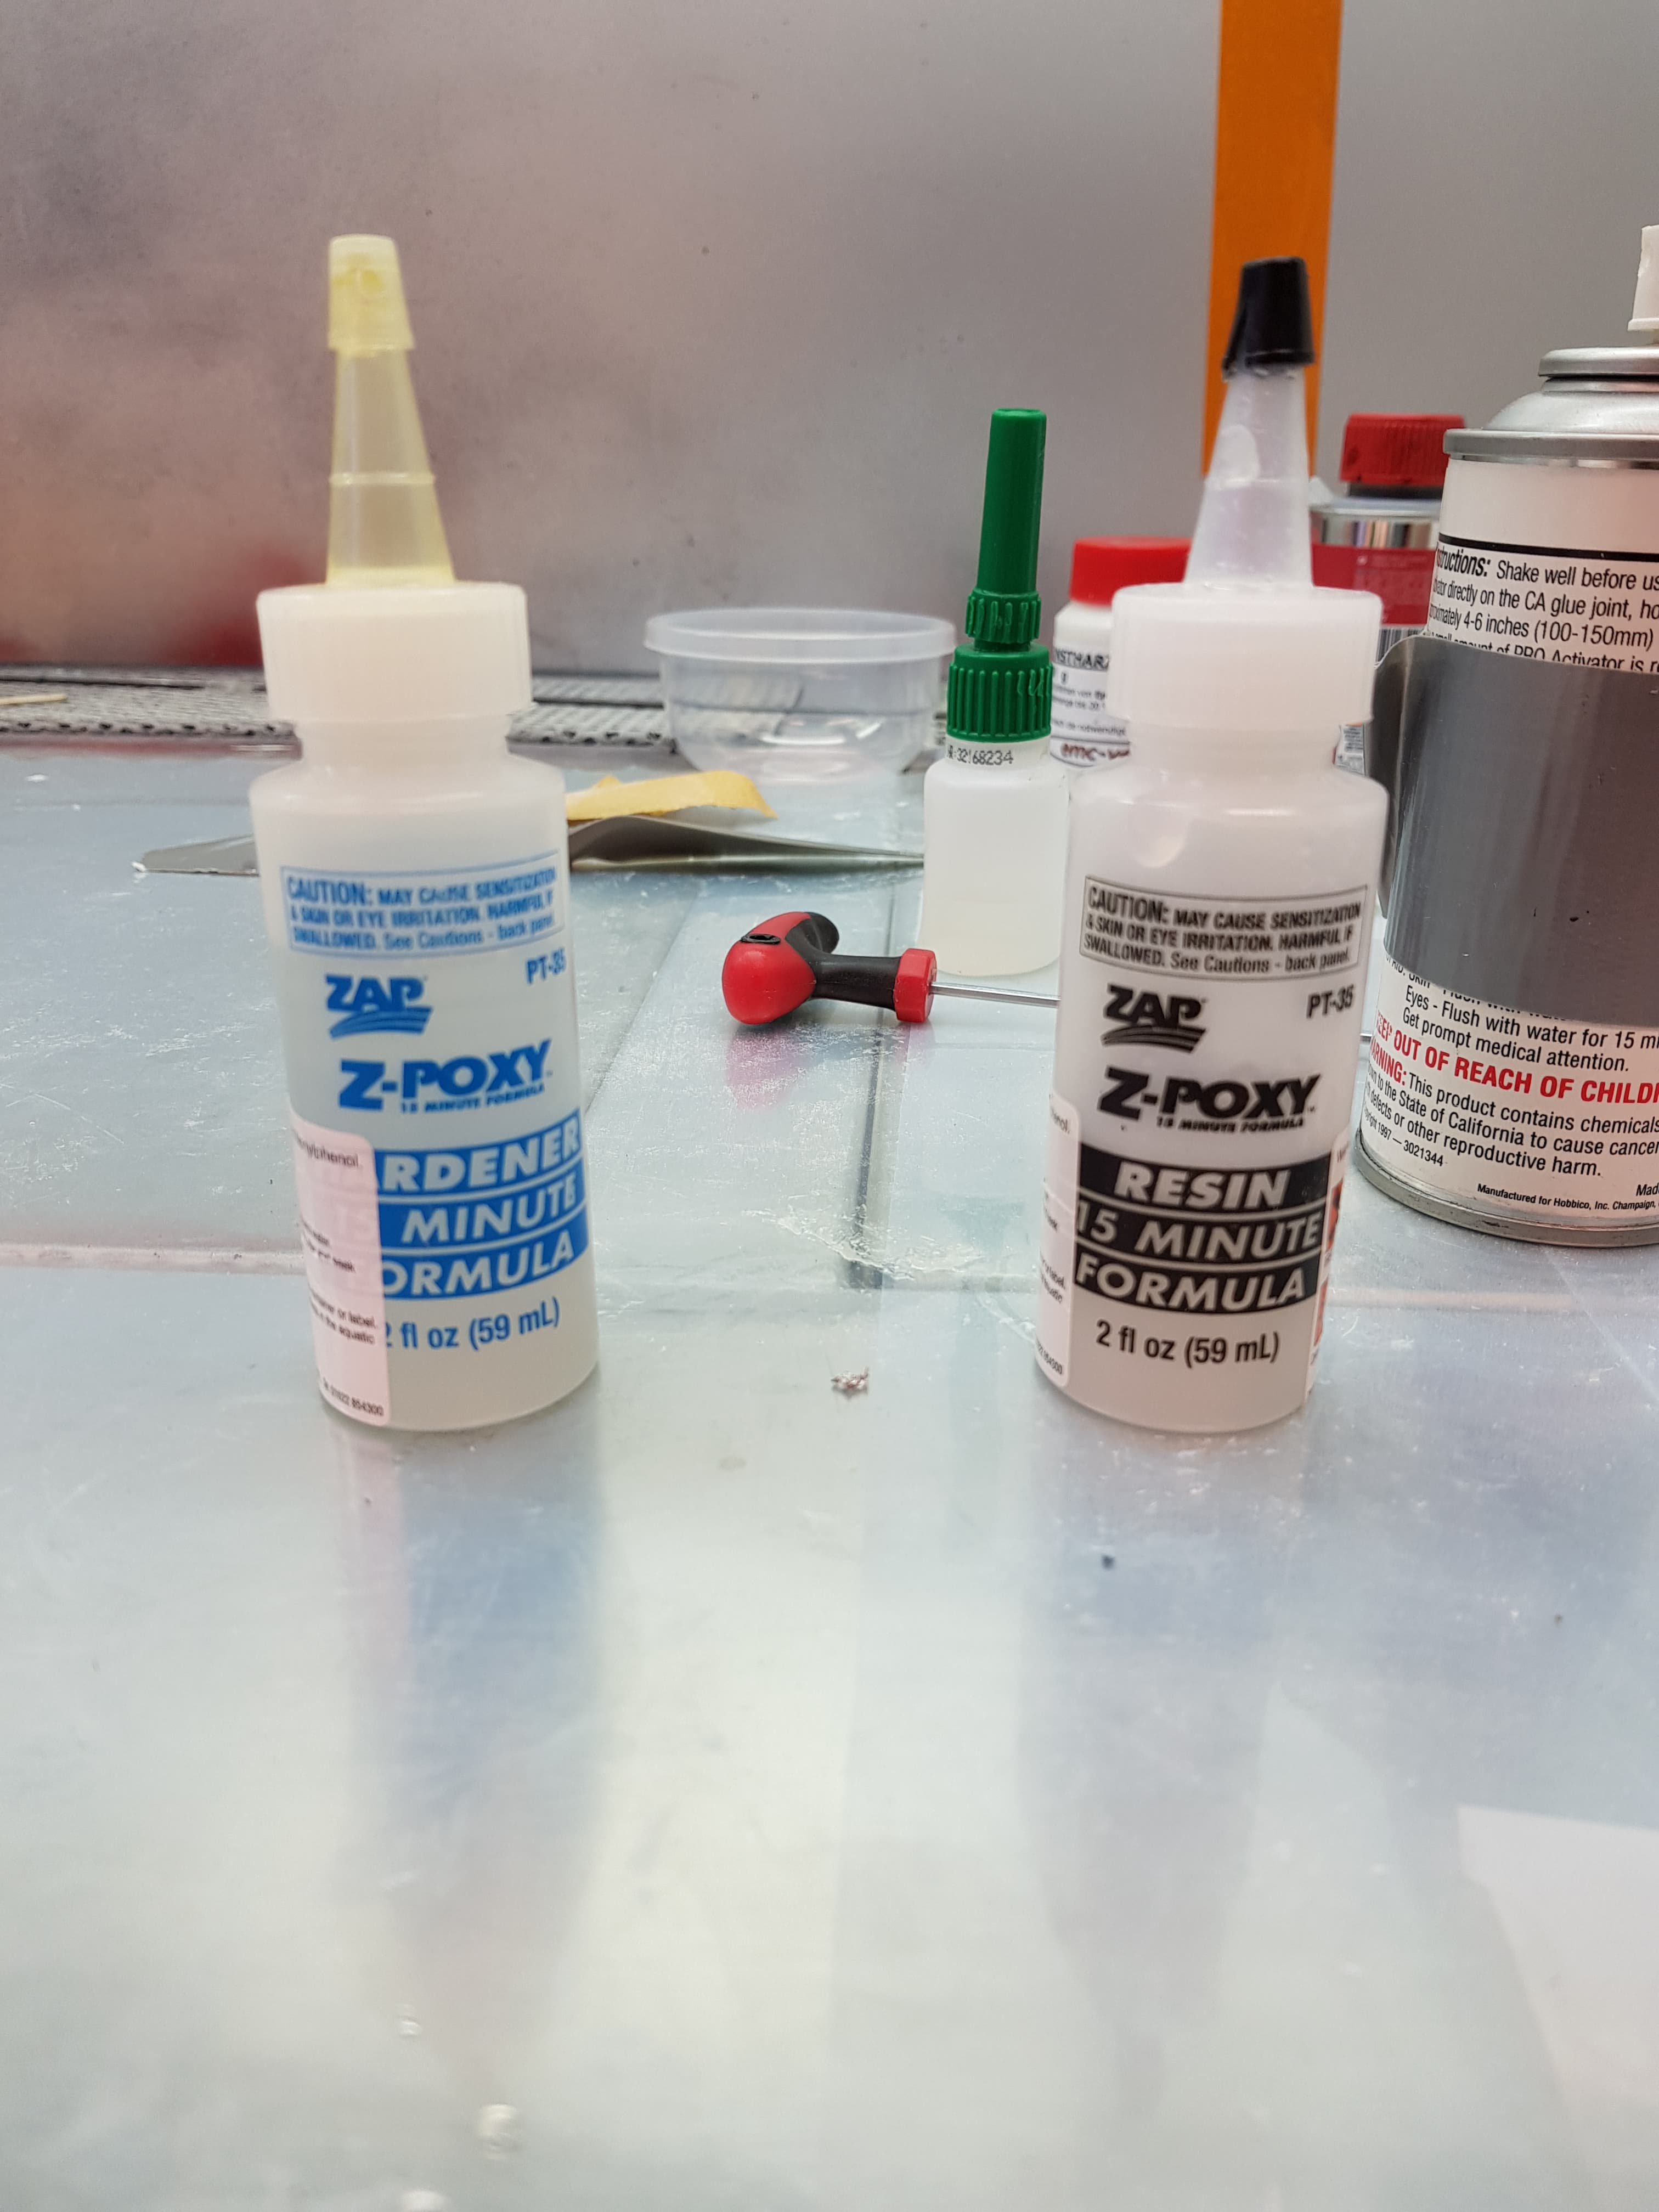
\includegraphics[width = .6\textwidth, height=9cm]{bilder/epoxyresin.jpg}
	\caption[Epoxy og herder]{Epoxy-lim består av to komponenter: resin og herder. Man skal etter Noruts retningslinjer ha opplæring ved bruk av disse stoffene, som inneholder kreftfremkallende stoffer. Svært liten opplæring om bruk og beliggenheter av utstyr i komposittlaben ble gitt. Det var tydeligvis ''underforstått'' at jeg visste hvordan jeg brukte disse stoffene på grunn av forelesninger. Det er verdt å merke at vi studenter på droneteknologi har ikke hatt noen innføring i HMS på kjemiske laboratorier.}

\end{figure}

\newpage
Man finner gjerne masse informasjon om bygging av fly på internett, men problemet mitt på dette var at jeg ikke er noe særlig god på praktisk arbeid. Jeg har for det meste vært av ``teoretisk karakter''. Men jeg synes det likevel er svært spennende å kunne gjøre noe praktisk arbeid. Usikkerheten min i hva jeg gjorde førte til at jeg ble skeptisk og usikker på om det jeg gjorde var faktisk rett. Det faktum at det ikke var noen som passet på at det jeg gjorde var riktig, gjorde at feil lettere slapp gjennom og ikke ble oppdaget før det eventuelt var for sent. Det var heller ingen annen av ingeniørene som var satt opp til å være en formell kontaktperson under byggingen, enn forskningssjef Rune Storvold. Ting ble dermed fort uorganisert og jeg visste dermed ikke hvem jeg skulle henvende meg til for veiledning. \\

Det var satt forutsetninger på ulike punkter, blant annet laging av sjekklister til flyene, noe som jeg ikke fikk vite skulle gjøres før den siste dagen av praksisen. Den ujevne opplysningsstrømmen gjorde at en god del dager ble unødvendig stressende og belastende. 

\subsection{Lærdom}
Til tross for det stressende arbeidsmiljøet fikk jeg lære hvordan man effektivt kan lime ulike materialer med hverandre, samt ulike typer limkompositter. Men jeg kan trygt si at det var lært på den harde måten. Den bakgrunnen jeg har fra emnene jeg har tatt så langt ved universitetet har hjulpet meg innenfor elektronikkforståelsen, men selve håndarbeidet og lignende har jeg erfaring fra hobbybasis.\\ Det er likevel ikke alt som jeg kan ved hjelp av de erfaringene jeg har så langt ta beslutninger på. Et eksempel er liming av ulike materialer til hverandre. Med andre ord, hvordan limstruktur som passer best, og hvordan man får best mulig fysisk binding mellom materialene. Mye av dette lærte jeg ved å lese på hobby-forum om hvordan andre har brukt ulike limsorter til ulike formål. \\

Jeg hadde satt som læringsmål for praksisperioden til å være å få et inntrykk i hvordan arbeidsdagen til en droneingeniør kunne være. Jeg har hatt muligheten i blant til å observere arbeidet som de ulike droneingeniørene på Norut jobbet med, og kjente mye igjen hva de jobbet med med tanke på teorien fra studiet. Men det store skillet på studiet og arbeidslivet er den praktiske biten. Studiet forbereder deg ikke til å gjøre praktisk arbeid. Læringskurven i det man kommer inn i bedriften blir dermed svært bratt for en periode hvis man ikke har hatt noe typer håndverks-erfaring fra før. Strengt tatt trengtes ikke så mye teori for å kunne gjennomføre prosjektet, men heller et praktisk anlegg.\\

Studiet gjør en ikke helt forberedt til denne typen arbeidsliv, noe som kan gjøre hoppet mellom skolebenken og jobb vanskelig. Jeg har i hvert fall fått lært at læringen stopper ikke etter utdannelsen. Den virkelige læringen kommer ute i arbeidslivet. \\

\newpage 
\section{Konklusjon}
Læringsmålet for min prakisperiode har jeg beskrevet til å være å få et inntrykk av en typisk arbeidsdag for en ingeniør. Ved hjelp av kunnskapen jeg hadde og den jeg opparbeidet meg under praksisen, klarte jeg å fremstille to fly på bestilling av Norut. Jeg har lært mye nyttig som jeg kan ta videre til andre prosjektoppgaver og arbeidsutfordringer i løpet av min yrkeskarriere. \\

En del ting kunne ha blitt gjort bedre for at perioden skulle vært mer organisert. En person med mindre til ingen erfaring i bygging, lodding eller annet praktisk arbeid ville etter min mening ha slitt med denne oppgaven. Likevel synes jeg det var moro og lærerikt å få bygge (mine første) ubemannede fixed-wings. \\

Å ha praksis som valgmemne vil jeg si var svært lurt, da man får den reelle smakebiten av en typisk ingeniørs arbeidsdag. Det samme får man bare ikke ved å sitte på skolebenken. Da jeg er av en mer teoretisk karakter enn praktisk, hjalp det veldig å oppleve dette. All kunnskapen jeg har opparbeidet meg gjennom perioden vil være nyttig til senere tider. 

\clearpage

\section{Kildehenvisning}
\begin{enumerate}
	\item Norut\\
		<\url{https://norut.no/nb}> Hentet \formatdate{30}{9}{2018}\\
	\item CryoWing Explorer\\
		<\url{https://bit.ly/2ygzkmC}> Hentet \formatdate{26}{9}{2018}\\
	\item CryoWing Scout \\
		<https://uit.no/Content/515073/artikkel1.pdf> Hentet \formatdate{26}{9}{2018}\\
	\item SkyWalker X8 \\
		Tatt av Rune Storvold, gitt på mail, hentet \formatdate{26}{9}{2018}\\
	\item DJI Inspire \\
		<\url{https://bit.ly/2PBIxNb}>Hentet \formatdate{26}{9}{2018}\\
	\item <\url{https://norut.no/nb/news/maritim-overvakning-folger-skipstrafikken-fra-drone}> \\ Hentet \formatdate{18}{10}{2018}\\

\end{enumerate}

Resten av bildene i rapporten er tatt via min telefon i løpet av praksisperioden.\\


\clearpage

\section{Vedlegg}
I dette kapittelet finner du følgende som kan være interessant å se. De tre siste vedleggene inneholder de tekniske dokumentene til luftfartøyet som jeg bygde. \\

Vedlegg nr.5 beskriver flyets struktur, med tanke på avionikk som skal monteres, rorutslag/defleksjon, hvordan man setter opp radiolink med mer. \\

Vedlegg nr. 6 er et dokument jeg skrev som veiledning til hvordan jeg skulle finne de ulike parameterne jeg skulle fylle ut i POH'en. \\

Vedlegg nr. 7 er et dokument som beskriver flyets oppbygning, begrensninger og eventuell annen informasjon som er viktig for piloten som skal operere luftfartøyet. 

\begin{enumerate}
	\item Attest fra Norut
	\item Praksisplan
	\item Logg av praksisperioden
	\item Mission Acceptance Form (UiT)
	\item CryoWing Observer RC-trainer byggelogg
	\item Determining capabilities for CryoWing Observer
	\item CryoWing Observer Pilot Operating Handbook
\end{enumerate}

\newpage

\begin{appendices}
\vspace*{8cm} \centering \section{Attest fra Norut}
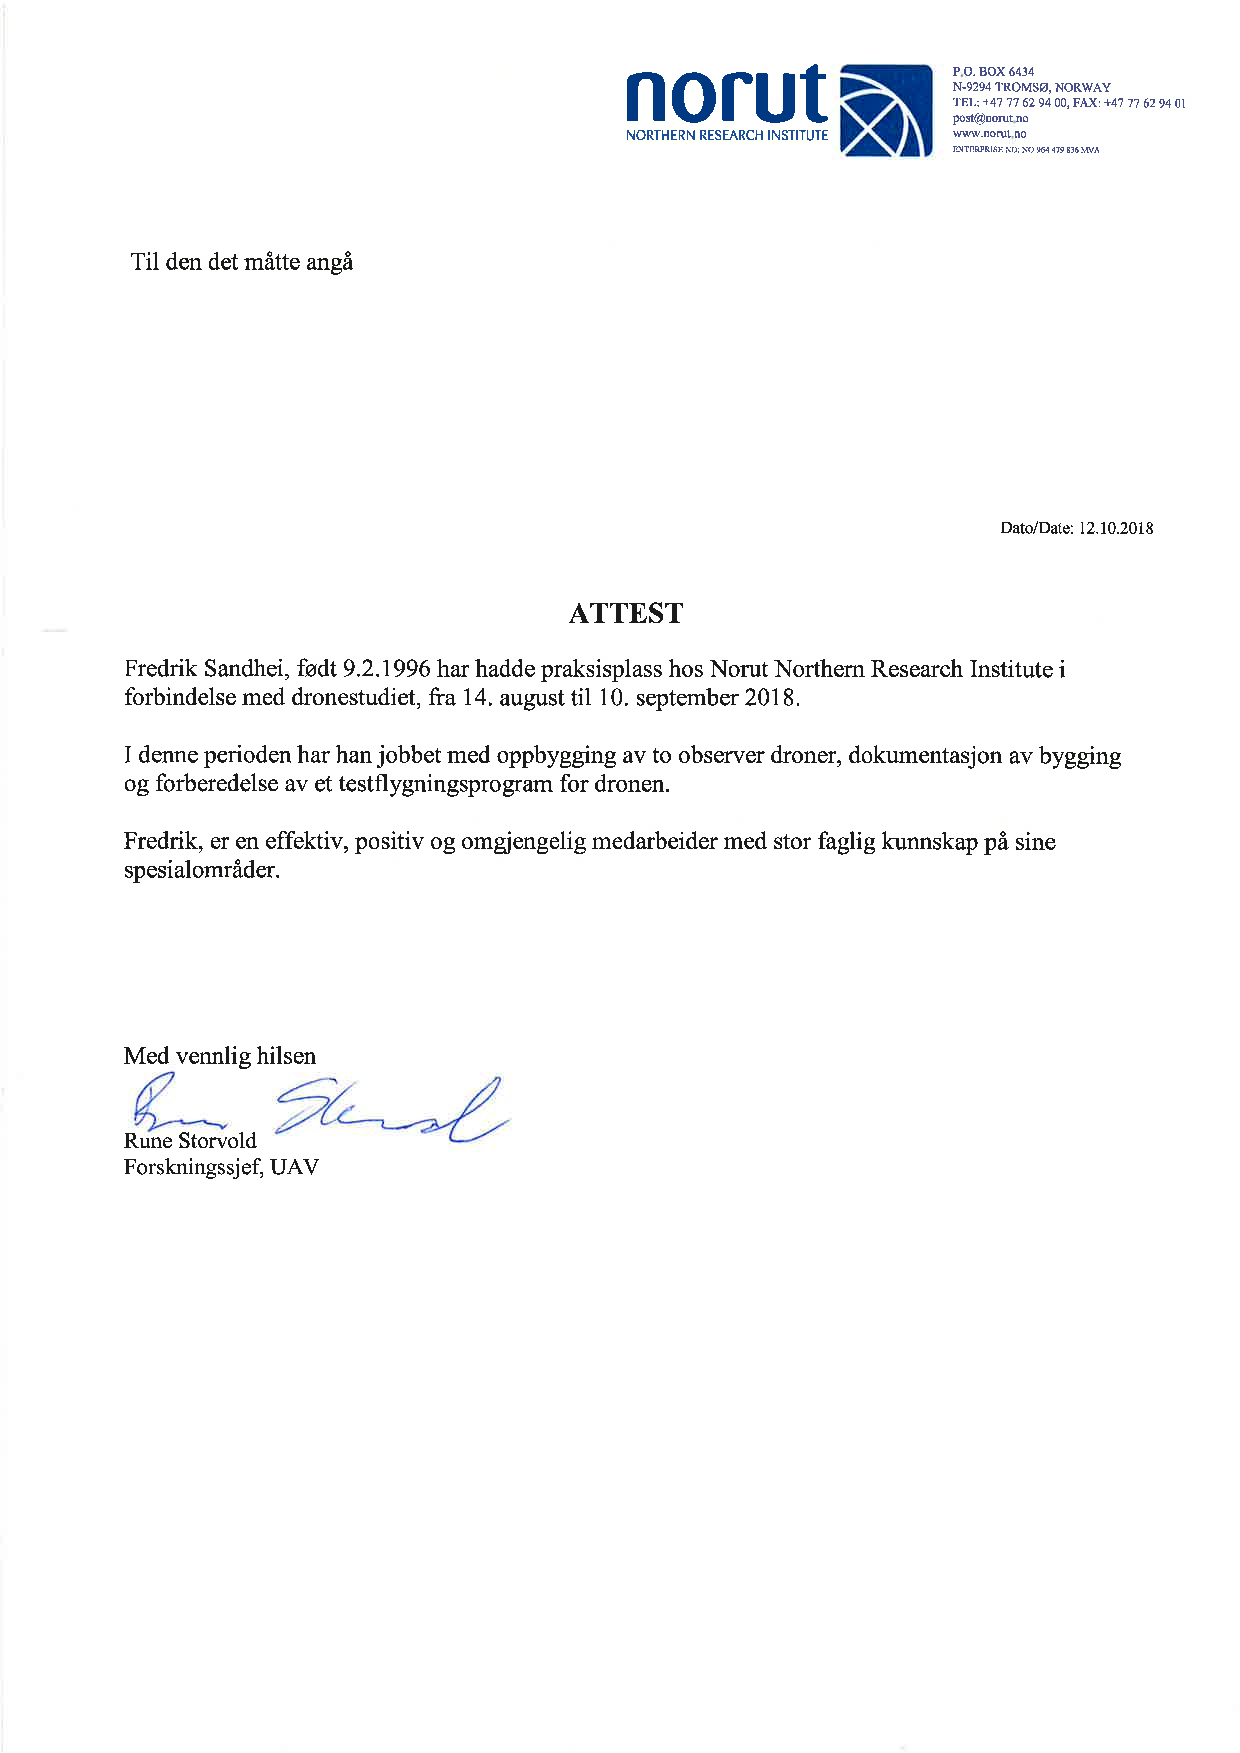
\includepdf[pages=-]{vedlegg/attest_Fredrik_Sandhei.pdf}
\vspace*{8cm} \centering \section{Praksisplan}
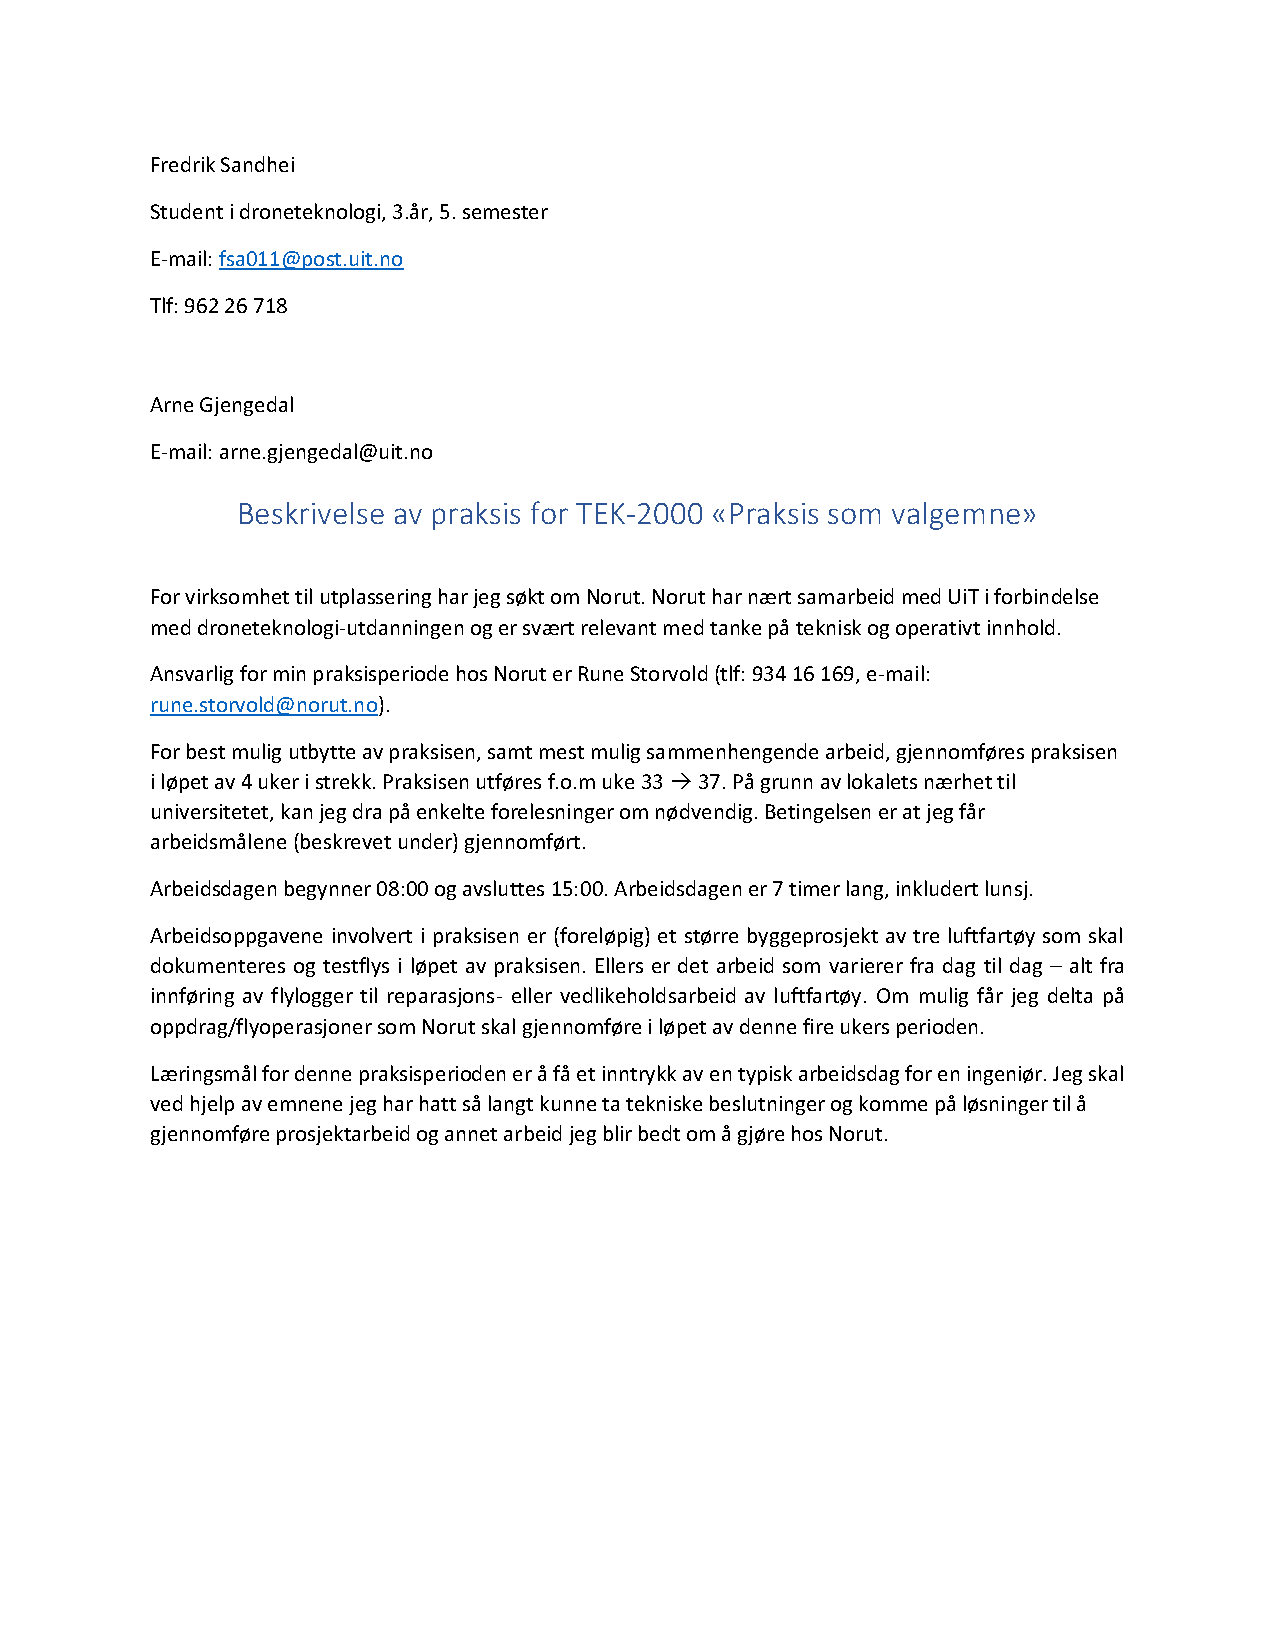
\includepdf[pages=-]{vedlegg/Beskrivelse_av_praksis_for_TEK.pdf}
\vspace*{8cm} \centering \section{Logg av praksisperiode}
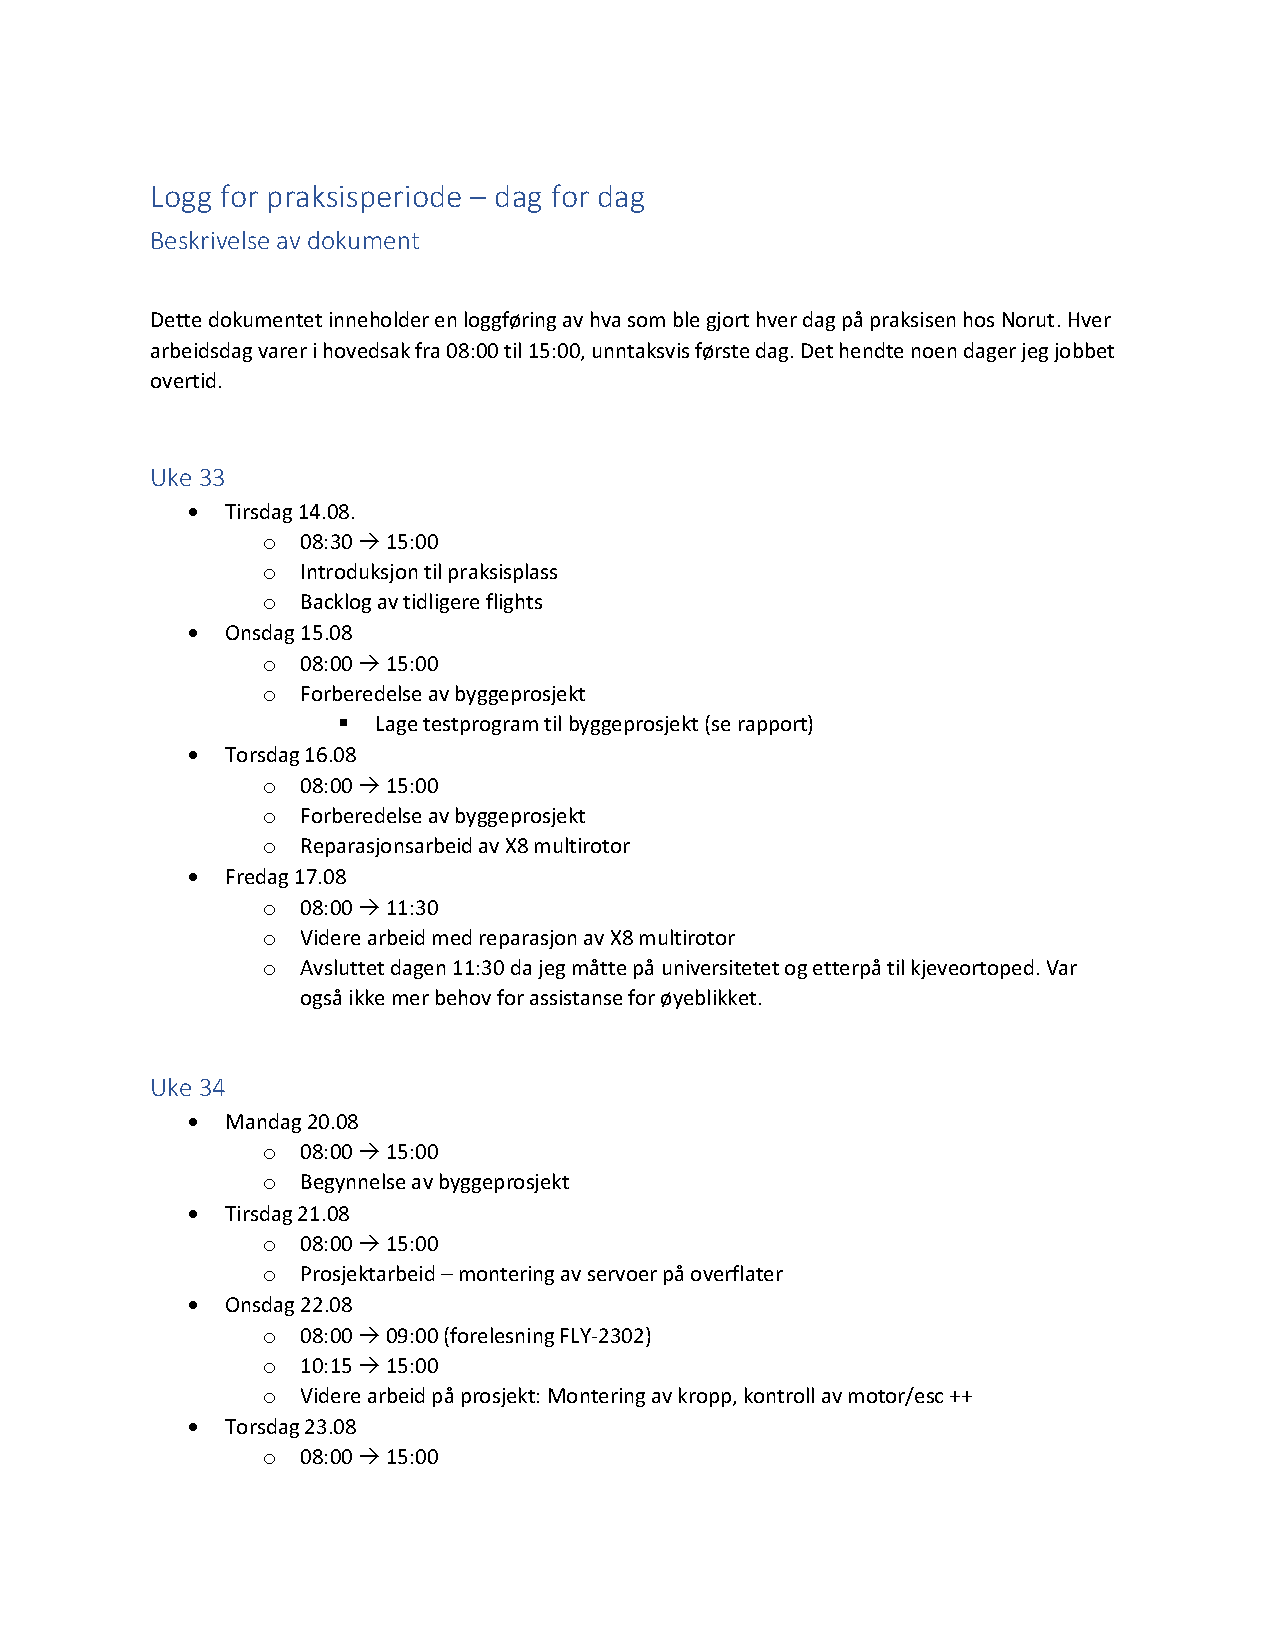
\includepdf[pages=-]{vedlegg/Logg_av_praksisperiode.pdf}
\vspace*{8cm} \centering \section{Mission Acceptance Form}
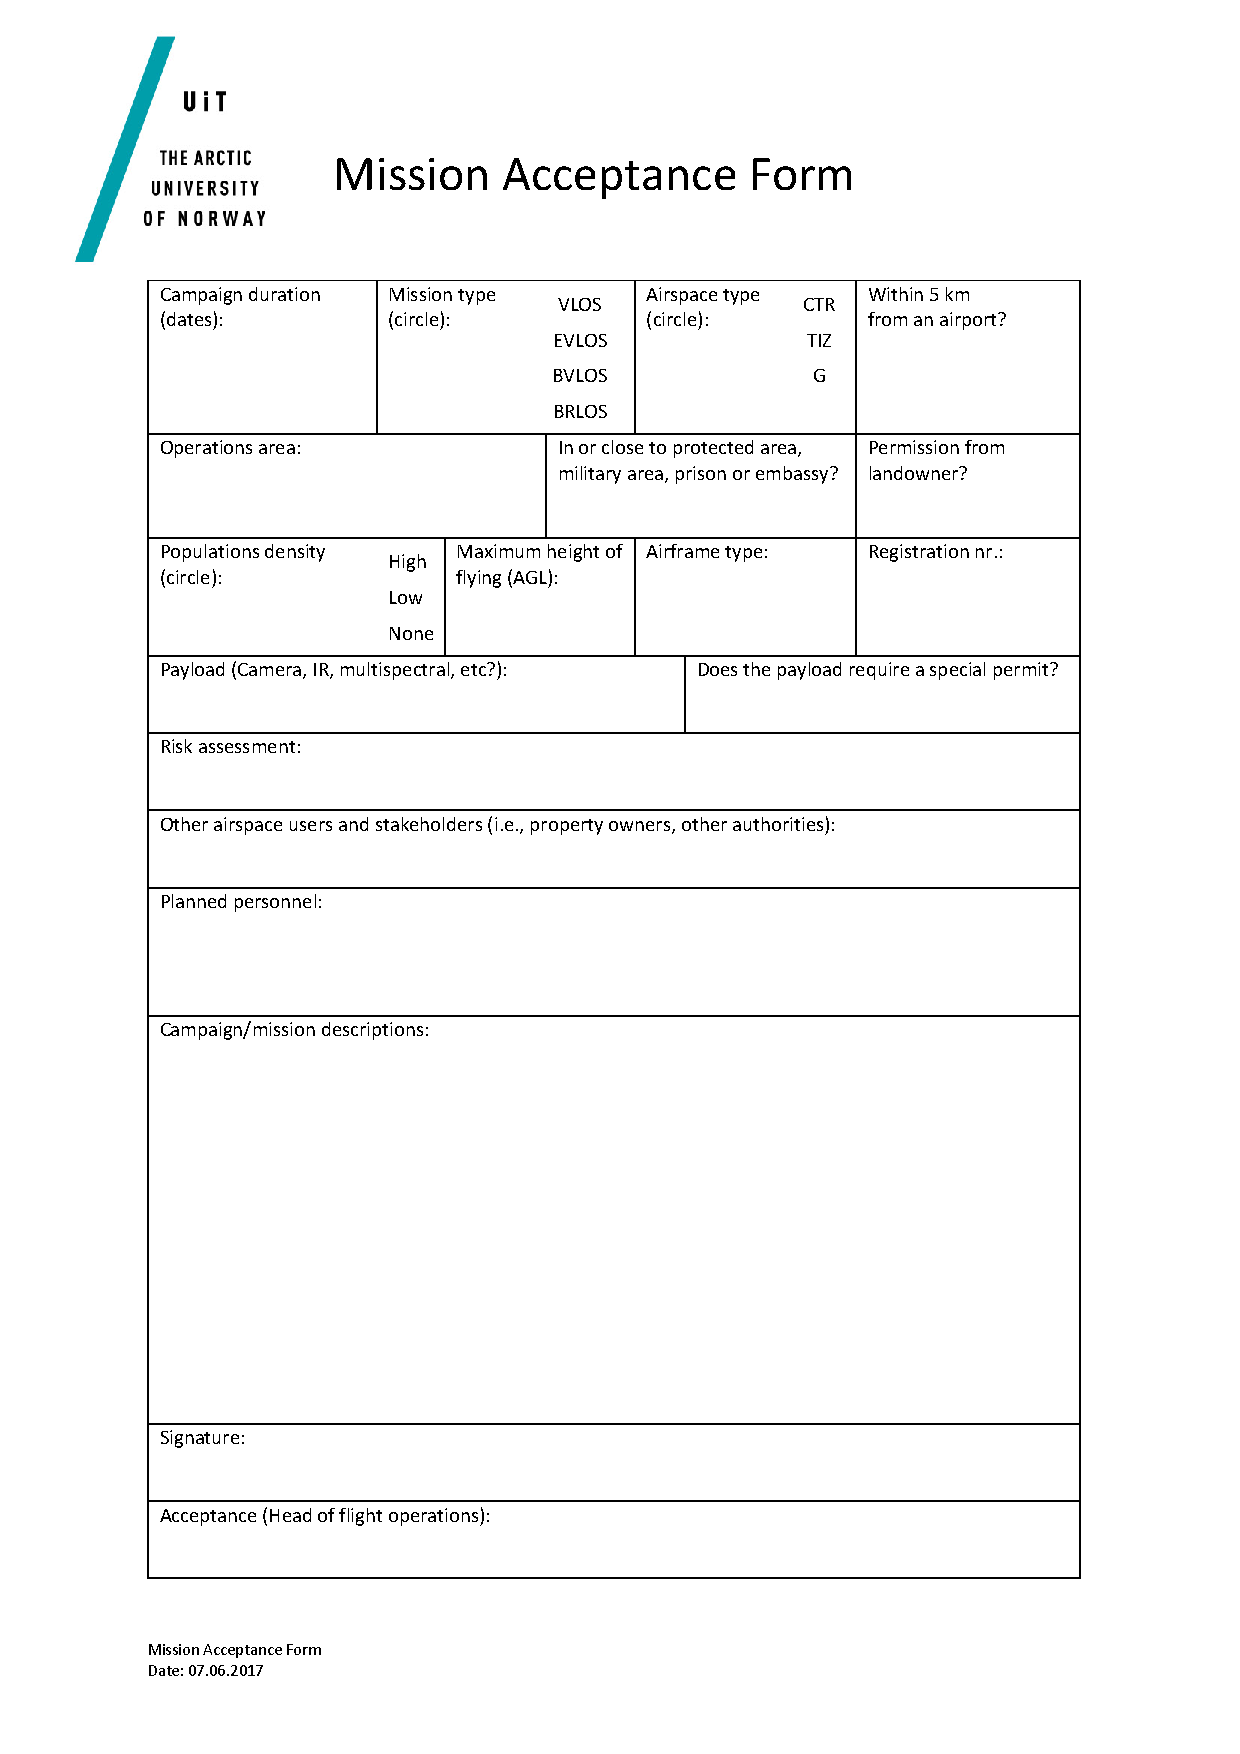
\includepdf[pages=-]{vedlegg/MissionAcceptanceForm.pdf}
\vspace*{8cm} \centering \section{CryoWing Observer byggelogg}
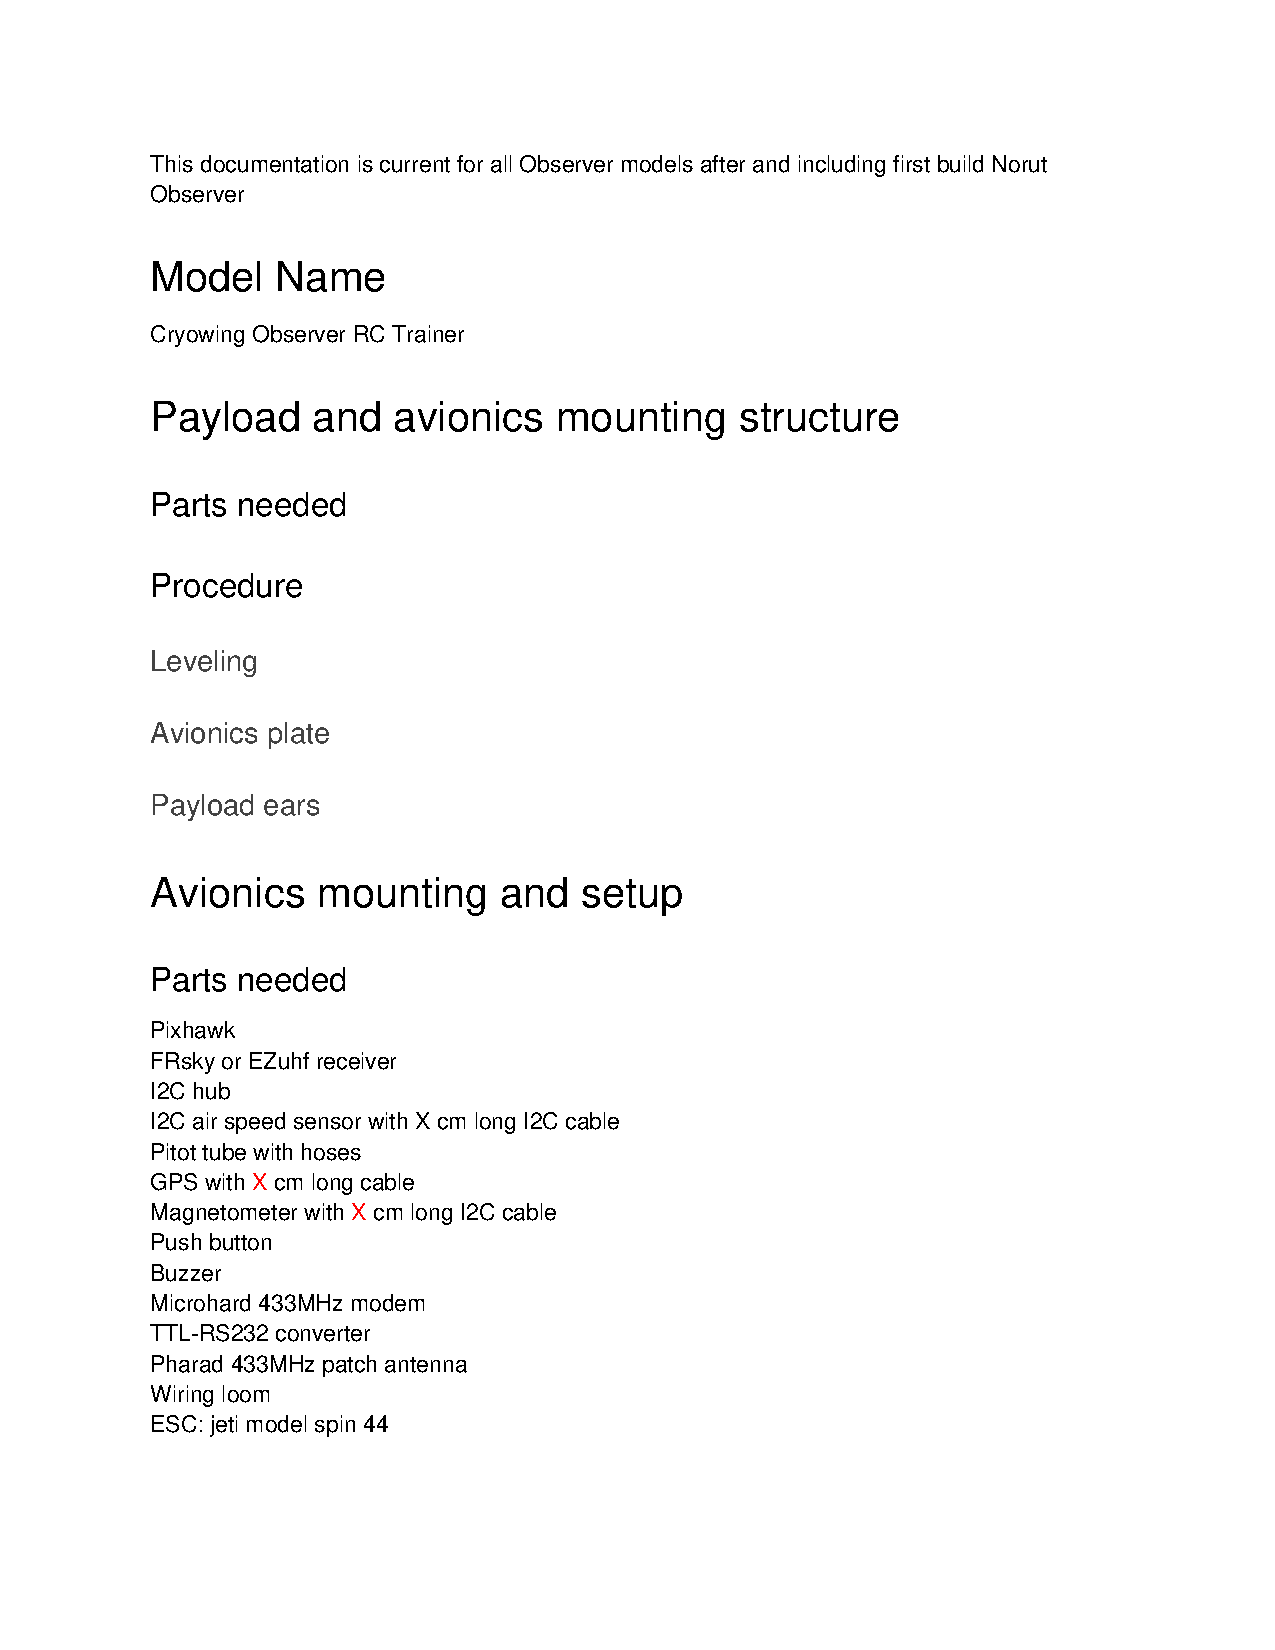
\includepdf[pages=-]{vedlegg/Observer_RC_Trainer_build_documentation.pdf}
\vspace*{8cm} \centering \section{Determining CryoWing Observer capabilities}
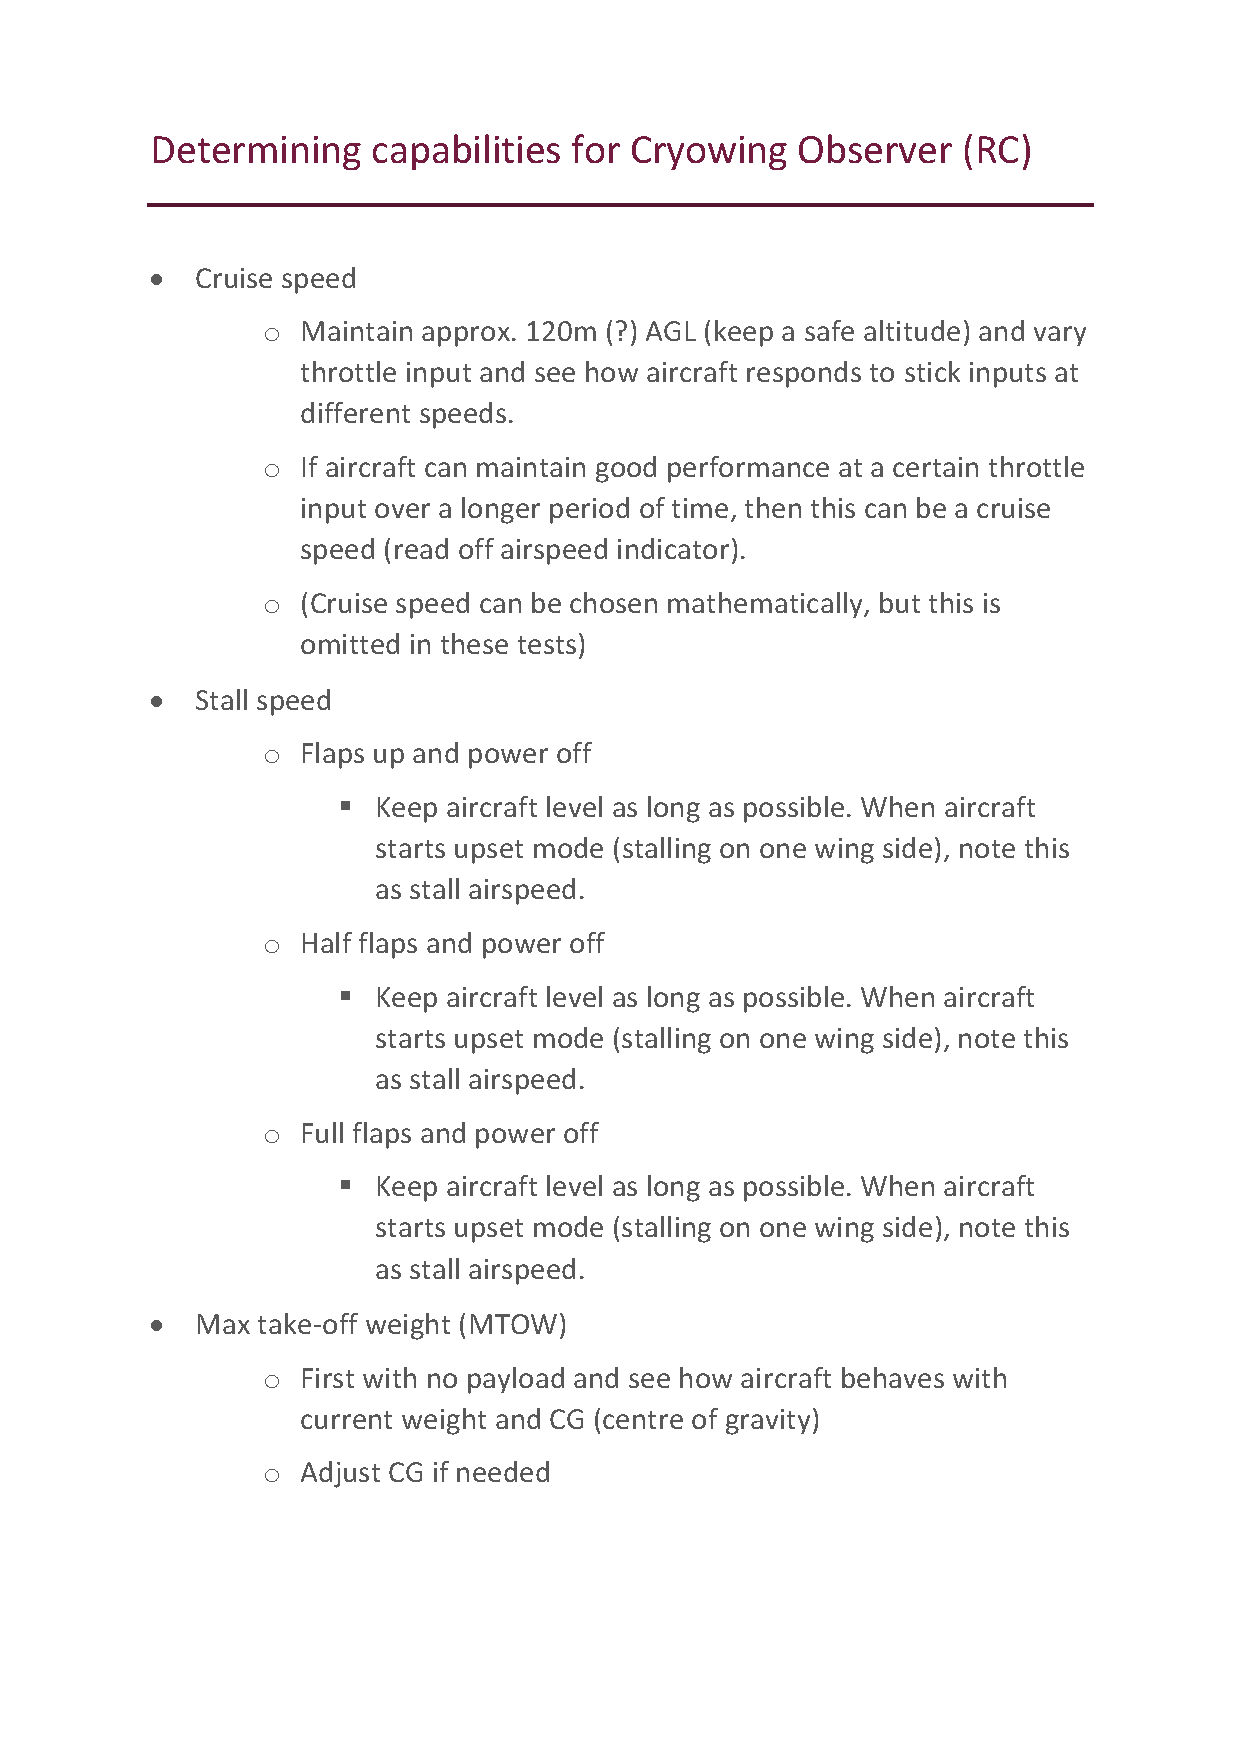
\includepdf[pages=-]{vedlegg/Determining_capabilities_for_Cryowing_Observer.pdf}
\vspace*{8cm} \centering \section{CryoWing Observer Pilot Operating Handbook}
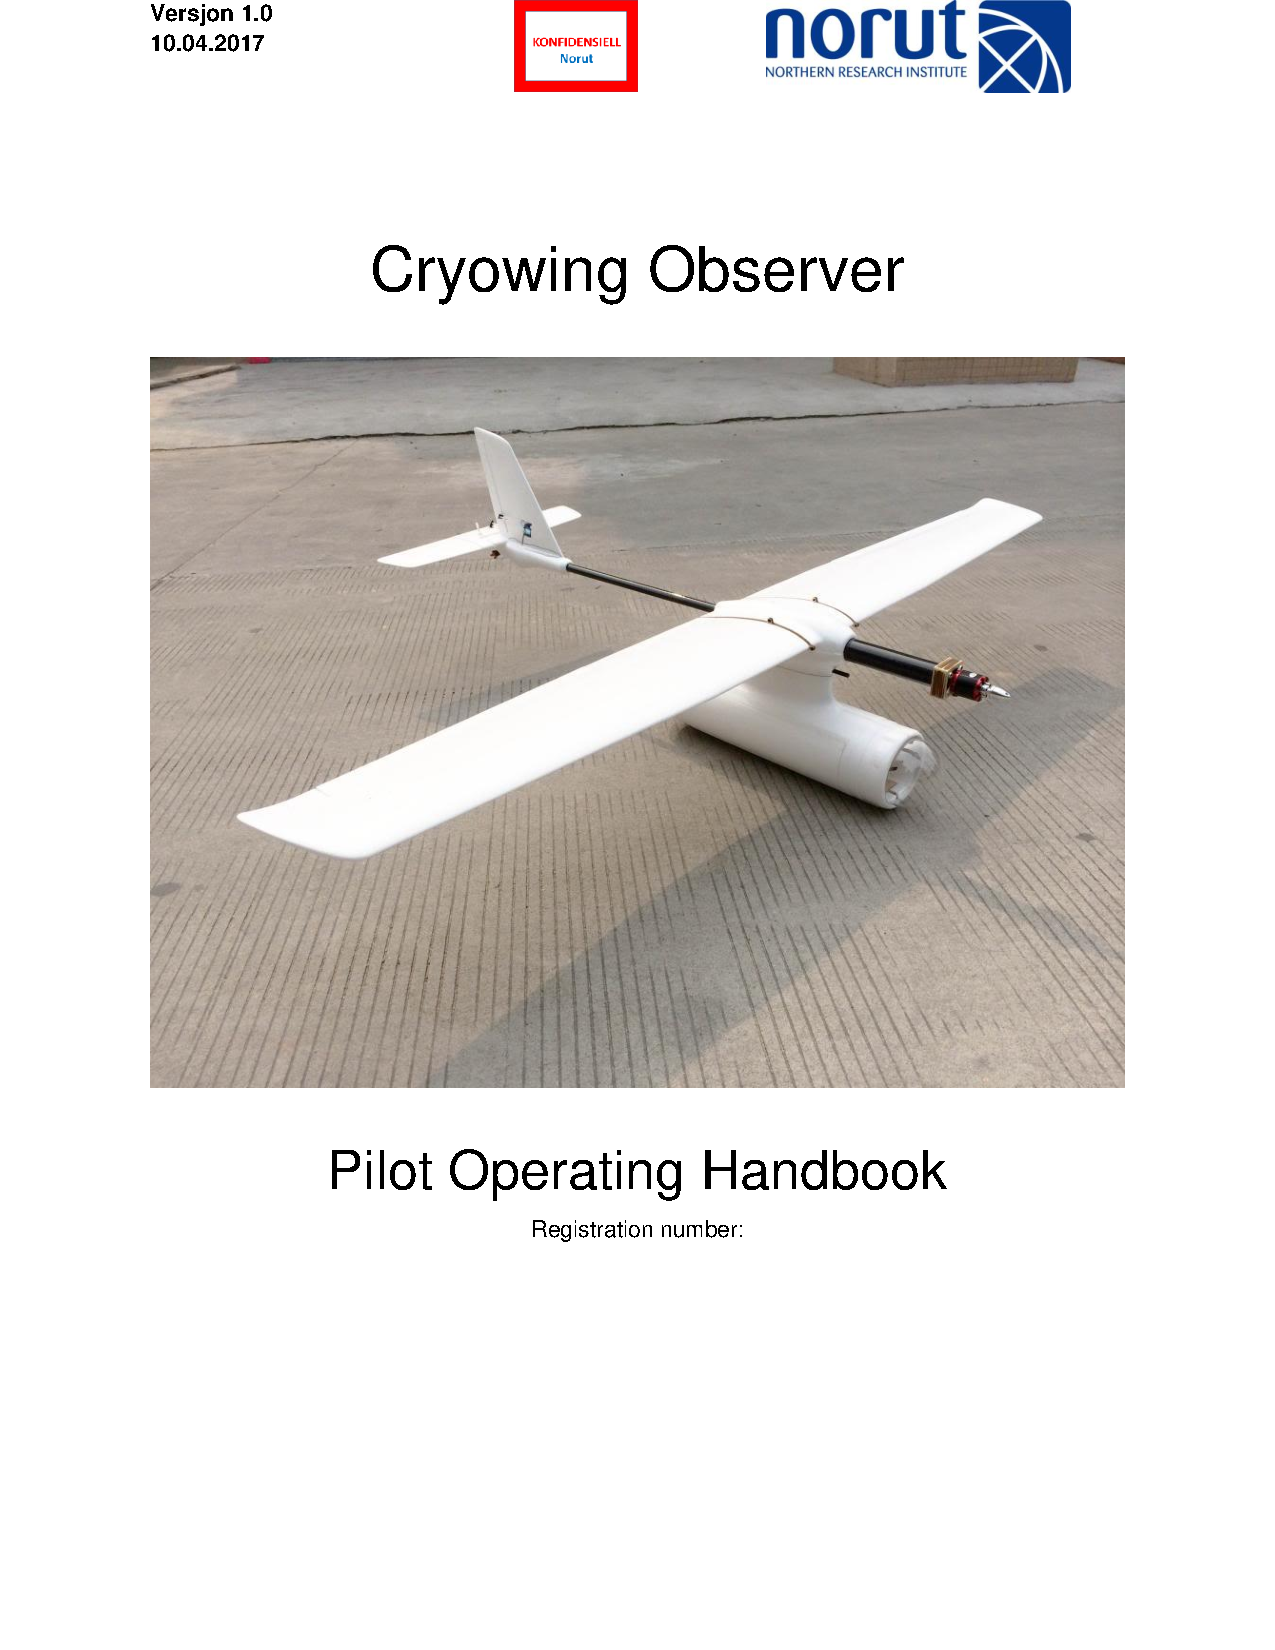
\includepdf[pages=-]{vedlegg/POH_Observer.pdf}
\end{appendices}

\end{document}